\chapter[Removing the Rubble:\\\phantom{Chapter 4:|}Jet Grooming and Cleanup Fish]{Removing the Rubble:\hfill\\Jet Grooming and Cleanup Fish}
\markboth{\small \textsc{Chapter \thechapter}: \bf Removing the Rubble: Jet Grooming and Cleanup Fish}{}

\label{chap:grooming}

% -----------------------------------
% Picturebook figure
% -----------------------------------
\reusefigure[]{picturebook_substructure}


We've now seen jets as proxies for partons, discussed the partonic cascade as a model of jet formation, and given some predictions regarding the jet observables and the flow of energy within jets.
%
We have also seen that there will be difficulties comparing these predictions to experimental results, in the form of low-energy pollution within particle collision events.
%
We now take a first step towards developing soft-insensitive probes of jet substructure, in order to gain information about the flow of energy in the partonic cascade in a more realistic experimental context.

In this chapter, we introduce \textit{\gls{jet-grooming}}:
%
a powerful and conceptually simple set of tools that facilitate our understanding of jet substructure by removing low-energy pollution from jets.
%
The low-energy phenomena of QCD that produce both soft contamination and \gls{additive-contamination} are notoriously difficult to model, and jet grooming has become an important toolkit used to empower both experimental and theoretical analyses of jet substructure
\cite{Krohn:2009th,Ellis:2009me,Larkoski:2014wba,Dasgupta:2013ihk,Dasgupta:2013via,Tseng:2013dva,Dasgupta:2016ktv,Thaler:2008ju,Thaler:2011gf,Hook:2011cq,Gallicchio:2011xq,Soper:2012pb,Gallicchio:2012ez,CMS-PAS-JME-09-001,CMS-PAS-EXO-09-002,CMS:2013kfa,ATL-PHYS-PUB-2009-081,ATL-PHYS-PUB-2010-008,Cui:2010km,ATLAS-CONF-2011-053,Chatrchyan:2013rla,Larkoski:2013eya,Dasgupta:2012hg,Backovic:2013bga,ATLAS-CONF-2013-084,Komiske:2018vkc,Komiske:2016rsd,Metodiev:2018ftz,Krohn:2012fg,MERINO:2013tta,Bhattacherjee:2016bpy,Macaluso:2018tck,Egan:2017ojy,Kasieczka:2017nvn,Pearkes:2017hku,Butter:2017cot,Catani:1992ua,Dokshitzer:1998kz,Dasgupta:2001sh,Banfi:2004yd,Banfi:2005gj,Ellis:2009su,Banfi:2010pa,Walsh:2011fz,Chien:2012ur,Li:2012bw,Jouttenus:2013hs,Hatta:2013iba,Larkoski:2014tva,Procura:2018zpn,Aaboud:2017aca,Frye:2016aiz, Almeida:2008yp,Larkoski:2017iuy,Larkoski:2017cqq,Thaler:2010tr,Abdesselam:2010pt,Katz:2010mr,Gallicchio:2010dq,Adams:2015hiv,Sirunyan:2017ezt,Moore:2018lsr,FerreiradeLima:2016gcz,Rubin:2010fc,Chatrchyan:2012sn,ATLAS:2019kwg,CMS-PAS-BTV-13-001,CMS-PAS-JME-13-006,Kribs:2009yh,Chen:2010wk,Hackstein:2010wk,Kim:2010uj,Almeida:2011aa,Pandolfi:2012ima,Vernieri:2014wfa,CMS-PAS-HIG-17-007,Procura:2014cba,ATL-PHYS-PUB-2019-027,Aad:2019vyi,ATLAS:2020gwe}.
%
Again, I also highly recommend the pedagogical treatment of \Reff{Marzani:2019hun}.



%==============================================
\section{The physical picture}
%==============================================

Examining the substructure of a jet is like peering through a cloud of rock dust or into a cloudy puddle to look for the faint gleam of a gem.
%
In particular, the high-energy structures within jets, which through \gls{asymptotic-freedom} encode partonic degrees of freedom, are obfuscated by a miasma of low-energy pollution.
%
To extract high-energy information encoded by jet substructure, we need to remove the low-energy pollution from \gls{hadronization}, \gls{deteffects}, \glslink{ue}{the underlying event}, and \glslink{pileup}{pileup} obfuscating any modern particle collision.
%
To uncover the physical properties of partons, we need to \textit{isolate} the high-energy structures within jets.


Jet grooming takes a very practical and straightforward approach to the problem of low-energy pollution:
%
it directly removes or modifies low energy particles from jets!
%
Grooming techniques help isolate the high-energy core of the jet that is directly associated with the hard scattering process, leading to cleaner and more accurate measurements of jet substructure.
%
In this context, grooming is crucial for realistic collider studies of QCD and new physics searches.

\begin{definitionbox}{Jet Grooming}{jet-grooming}
    \glslink{jet-grooming}{\vocab{Jet grooming}} is any method that modifies the constituents of a jet -- e.g. by removing, reweighting, or reclustering certain particles -- in order to reduce the impact of \glspl{soft-distortion} and \gls{additive-contamination}.
    %
    Jet grooming usually aims to preserve the information associated with the high-energy partonic physics of jet production.
\end{definitionbox}

The conceptual simplicity of jet grooming is accompanied by several practical benefits.
%
Jet grooming can be used to address many sources of low-energy pollution at once, leading to simple analyses that yield robust experimental jet substructure results.
%
Appropriately designed jet grooming strategies can even facilitate analytic calculations of jet substructure observables that may have otherwise involved complicated regions of phase space, or allow the analytic prediction of traditionally mystifying \gls{hadronization} effects \cite{Larkoski:2014wba}.


Jet grooming must also be computationally efficient.
%
High-energy particle accelerators collect data from \textit{more than 500 million collision events every second}.%
\footnote{
    This is a concern because jet grooming is used in experimental trigger systems, which filter among these half-a-billion events which ones should be stored in the memory of a particle collision database.
    %
    The given number is from \href{http://lhc-machine-outreach.web.cern.ch/collisions.htm}{\texttt{the CERN website}}, and does not account for fluctuations in the number of collisions.
}
%
In order to meet the needs of modern particle physicists, jet grooming algorithms must be as fast as possible in order to parse through our vast mountains of data.


There is one final feature we will discuss that is desirable for jet grooming procedures, but that is deceptively difficult to achieve:
%
\textit{continuity}.


The principle of \gls{lphd}, discussed in \Def{lphd}, suggests that small changes in hadronic energy flow should be associated with small changes in the associated partonic degrees of freedom, and vice versa.
%
Therefore, we will hope to achieve a way of isolating high-energy, partonic information in a \textit{continuous} way:
%
small changes in the flow of energy within a jet should not drastically affect what we infer about partonic degrees of freedom.
%
Conversely, a jet grooming algorithm is \textit{discontinuous} if small changes in the properties of jet constituents, such as their energies or angular positions, can lead to extensively different groomed results.

The more specific examples of \textit{soft continuity} and \textit{angular continuity}, mentioned briefly in Remark~\ref{rem:continuity}, will play a significant role in this chapter:
\begin{definitionbox}{Soft and Angular Continuity}{}
    A collider observable \(X\) is \vocab{\glslink{soft-discontinuity}{soft continuous}} (\vocab{\glslink{angular-discontinuity}{angularly continuous}}) if it is continuous with respect to changes in the energies (angles) of final-state particles.

    Conversely, a collider observable \(X\) is \vocab{soft discontinuous} (\vocab{angularly discontinuous}) if infinitesimal changes in the energies (angles) of final-state particles can cause large changes in the value of \(X\).
\end{definitionbox}
\noindent
We will provide more precise definitions of continuity in \Sec{emd}, where we discuss the continuity of grooming algorithms as maps on the space of energy flows.



Unfortunately, traditional jet grooming algorithms are discontinuous, as we discuss in detail in \Sec{discontinuity} (and as in, for example, \Reffs{Dasgupta:2013ihk,Larkoski:2014wba}).
%
Discontinuous behavior in jet grooming algorithms leads in turn to undesirably sensitive responses to low-energy pollution.
%
Experimentally, discontinuities in grooming lead to large responses of groomed substructure to the interactions of jets with experimental detectors, and resulting difficulties in unfolding \cite{ATL-PHYS-PUB-2019-027,Aad:2019vyi,ATLAS:2020gwe}.
%
Theoretically, discontinuities in grooming lead to uncertainties in fixed-order calculations \cite{Larkoski:2014wba} and complications in describing the effects of \gls{hadronization} on groomed jet substructure \cite{Hoang:2019ceu}.


In order to create continuous methods for extracting high-energy information from jets, we introduce the paradigm of Pileup and Infrared Radiation Annihilation (\PIRANHA{}) for \emph{continuous jet grooming}, introduced by myself and my collaborators in \Reff{Alipour-Fard:2023prj}.
%
The \PIRANHA{} paradigm utilizes lessons from traditional jet grooming together with geometric intuition from optimal transport -- see e.g. \Sec{emd} -- in order to generate more continuous grooming strategies, with better formal and phenomenological behavior.
%
However, though we achieve the goal of continuous grooming through the framework of \PIRANHA{}, we will see that as we make grooming procedures which are more and more continuous, they become less and less malleable for interpretation in perturbative calculations.
%
Indeed, without some very subtle work, \textit{any} grooming procedure which attempts to utilize the tree-like structure of partonic emissions discussed in the previous chapter will be necessarily discontinuous (see \Sec{ang_discont}).


\remark{jet-discontinuity}{
    All observables depending on a jet definition are technically angularly discontinuous because the angles between particles determine, discontinuously, whether a jet algorithm reconstructs them as ling within the same jet.
    %
    Therefore, whenever we use the terms ``soft (angular) continuous'', we implicitly mean ``soft (angular) continuous up to discontinuities associated with jet boundaries/the jet definition itself.''
}


\begin{table}[t]
    \centering
    \begin{tabular}{|c|c||c|c||c|c|}
\hhline{~~--||--}
\multicolumn{2}{c|}{}
&
\multicolumn{2}{c||}{Safety}
&
\multicolumn{2}{c|}{Continuity}
\\
\hhline{~~--||--}
\noalign{\vskip\doublerulesep
         \vskip-\arrayrulewidth}
\hhline{--||--||--}
    Groomer & Acronym &
    Infra-red & Collinear &
    Soft & Angular
\\
\hhline{--||--||--}
\noalign{\vskip\doublerulesep
         \vskip-\arrayrulewidth}
\hhline{--||--||--}
Apollonius Subtraction & P-AS &
\cmark & \cmark &
\cmark & \cmark
\\
\hhline{--||--||--}
Iterated Voronoi Subtraction & P-IVS &
\cmark & \cmark &
\cmark & \cmark
\\
\hhline{--||--||--}
Recursive Sub. w/Fraction \(f = 1/2\) & \PRSF{1/2} &
\cmark & \cmark &
\cmark & \danger
\\
\hhline{--||--||--}
Recursive Sub. w/Fraction \(f \neq 1/2\) &  P-RSF\(_{f \neq 1/2}\) &
\cmark & \cmark &
\danger & \danger
\\
\hhline{--||--||--}
\noalign{\vskip\doublerulesep
         \vskip-\arrayrulewidth}
\hhline{--||--||--}
Soft Drop (SD), \(\beta_{\rm SD} > 0\) & SD\(_{\beta > 0}\) &
\cmark & \cmark &
\xmark & \danger
\\
\hhline{--||--||--}
SD (grooming mode), \(\beta_{\rm SD} \leq 0\) & SD\(_{\beta \leq 0}\) &
\cmark & \xmark &
\xmark & \danger
\\
\hline
\end{tabular}


    \caption[Safety and continuity properties of the \PIRANHA{} and Soft Drop grooming algorithms.]{
    Safety and continuity properties of the \PIRANHA{} and Soft Drop grooming algorithms studied in this chapter.
    %
    The mark \cmark~indicates that a groomer satisfies the associated condition, while the mark \xmark~indicates that it does not.
    %
    The mark \raisebox{0.15 em}{\danger} indicates that a groomer does not satisfy the condition, but only in a boundary region of phase space that is exponentially suppressed at leading order in perturbative QCD.
    %
    The mark \raisebox{0.15 em}{\danger} indicates that a groomer does not satisfy the condition, but only in a boundary region of phase space that is exponentially suppressed at leading order in perturbative QCD.\footnotemark
    }
    \label{tab:groomerlist}
\end{table}

\Tab{groomerlist} expresses the infra-red/collinear safety (using the definition of \Reff{Komiske:2020qhg}) and soft/angular continuity properties of the traditional and \PIRANHA{} groomers we discuss in this paper.
%
The soft continuity properties expressed in \Tab{groomerlist} are simple to understand by comparing the hard-cutoff framework of popular groomers to the subtractive framework of \PIRANHA{}.
%
The angular discontinuities expressed in \Tab{groomerlist} are more subtle and are inherited from angular-ordered jet clustering.
%
We note that the Recursive Subtraction algorithms (P-RS) we introduce are discontinuous only in a highly suppressed region of phase space, and we still find it suitable to call P-RS a family of \PIRANHA{} groomers.


In the remainder of the chapter, we show that grooming can provide a useful and intuitive way to extract high-energy information from jet substructure.
%
We exposit the physics of traditional, hard-cutoff grooming in \Sec{traditional-grooming} before exploring \PIRANHA{} strategies for continuous grooming in \Sec{piranha}.
%
We emphasize the improved continuity of \PIRANHA{} formally in \Sec{discontinuity} and in practical applications in \Sec{grooming-pheno}.





%==============================================
\section{Seeing Deep by Keeping Clean: Traditional Jet Grooming}
%==============================================
\label{sec:traditional-grooming}

    % These grooming methods are essential in ensuring that the jet substructure measurements are more representative of the original parton shower, particularly in high-luminosity environments where \glslink{pileup}{pileup} is a significant challenge.


% \begin{remarkbox}{Grooming for Quark-Gluon Discrimination}{}
%     One of the primary applications of jet grooming is to improve quark-gluon discrimination. Quark jets tend to be more collimated with fewer subjets, while gluon jets are broader and more multi-pronged. Grooming techniques such as trimming and pruning remove soft radiation that could distort the substructure, making it easier to distinguish between quark- and gluon-initiated jets. This discrimination is particularly useful for searches in particle physics, where understanding the partonic origin of jets can shed light on underlying processes.
% }

% \begin{remarkbox}{Impact of Jet Grooming on Pileup Mitigation}{}
%     Pileup radiation, which results from additional proton-proton collisions, can have a significant impact on jet substructure in high-luminosity environments. Grooming algorithms are specifically designed to mitigate this effect by removing low-energy particles and focusing on the core hard-scattering part of the jet. For instance, trimming removes soft and wide-angle radiation from \glslink{pileup}{pileup} interactions, thus improving the resolution of jet observables and reducing the bias introduced by \glslink{pileup}{pileup}. As a result, groomed jets are more reliable in precision measurements, such as the study of top quarks and Higgs bosons.
% }


A traditional and elegant approach to jet grooming is to provide a hard cutoff on the energy of the radiation within a jet;
%
this approach retains high-energy information, removes radiation that may be sensitive to \glspl{soft-distortion} or due to \gls{additive-contamination}, and even facilitates perturbative calculations of jet substructure observables.


In this section, we introduce traditional hard-cutoff techniques for jet grooming, discuss their properties, and understand some analytic features of traditionally-groomed jets.
%
We begin with an extremely simple -- and not impractical -- grooming procedure that is nonetheless similar to more complicated algorithms.
%
We then focus on \glsentrylong{soft-drop} -- an algorithm for jet grooming which is extremely popular due to its simplicity, efficiency, and flexibility.%
\footnote{
    Other traditional grooming algorithms include filtering, trimming, pruning \cite{Dasgupta:2013ihk}, and some algorithms for boosted object tagging \cite{CMS-PAS-JME-09-001}, and have similar formal properties to Soft Drop -- including the use of reclustering and the presence of discontinuous behavior.
}

Traditional jet grooming algorithms are discontinuous, but we will only briefly touch on the effects of their discontinuous behavior in this section.
%
Therefore, readers familiar with hard-cutoff jet grooming algorithms such as Soft Drop may want to skip to \Sec{discontinuity}, where we discuss the soft discontinuities of the Soft Drop algorithm.
%
In \Sec{grooming-pheno}, we will see the enormous effects of discontinuities in practical applications.


% ---------------------------------------
\subsection{The Constant Cutoff: An Invitation to Jet Grooming}
% ---------------------------------------
\label{sec:constant-cutoff}

The goal of jet grooming is the efficient removal of low-energy pollution.
%
A simple strategy is to throw away any jet constituents with an energy \(E < E_\text{cut}\), for some constant \(E_\text{cut}\).
%
This is a reasonable first step, and indeed removes low energy radiation to form a resulting groomed jet.

However, we can develop a better algorithm which leverages the tree structure of the partonic cascade and is therefore more amenable to resummed calculations.
%
Instead ignoring particles with \(E < E_\text{cut}\), we will re-cluster the jet to produce a tree-structure representative of the partonic cascade.
%
Then, we will recursively \glslink{declustering}{de-cluster} the jet, throwing out branches of the jet tree with a soft energy fraction less than a pre-defined threshold, \(z < \zcut\).
%
We call this algorithm the \textit{\gls{constant-cutoff}} algorithm for jet grooming.


\begin{definitionbox}{Constant Cutoff Grooming Algorithm}{constant-cutoff}
    The \vocab{constant cutoff grooming algorithm} is a map which takes in a jet and returns a new, \textit{groomed} jet.
    %
    It depends on a single parameter \(\zcut \in (0, 1/2)\).

    The constant cutoff algorithm acts on a jet via the following procedure:
    \begin{enumerate}
        \item
            Re-cluster the jet using the angular-ordered C/A algorithm, as discussed in \Sec{reclustering}, and begin \gls{declustering} the jet tree, starting at the base;

        \item
            If the current branch is a final state particle and cannot be \glslink{declustering}{de-clustered}, stop the algorithm;
            %
            otherwise \glslink{declustering}{de-cluster} the current branch into a softer emission with energy fraction \(z\) of the current branch, and a harder emission with energy fraction \(1-z\);

        \item
            If \(z < \zcut\), remove the softer branch from the jet and continue the algorithm recursively by declustering the remaining, harder branch, as in Step 2;

        \item
            Otherwise, if \(z \geq \zcut\), continue recursively by \gls{declustering} \textit{both} the softer and the harder branch.
    \end{enumerate}
\end{definitionbox}

    The constant cutoff grooming algorithm removes the results of any particularly soft partonic emissions from the jet.
    %
    Its recursive definition in terms of the energy fractions \(z\) of a \glslink{reclustering}{re-clustered} jet tree facilitates resummed calculations, allowing us to model its action on jets through its action on the LL tree of partonic emissions.
    %
    This toy jet grooming example is quite similar to Soft Drop, a widely used grooming algorithm explored in \Sec{softdrop}, and will be a nice playground for building intuition.
    %
    Indeed, the constant cutoff grooming algorithm is the \(N \to \infty\) limit of recursive Soft Drop with \(\betasd=0\) \cite{Dreyer:2018tjj}.

\begin{exercise}{}{}
    Is the \gls{constant-cutoff} algorithm an \glslink{irc-safety}{IRC safe} collider observable?
\end{exercise}



%\remark{}{
%    %
%    Low-energy degrees of freedom are very likely to be groomed by the constant cutoff algorithm;
%    %
%    while \(z > \zcut\) does not imply \(E > E_\text{cut}\) for any value of \(E_\text{cut}\),
%    %
%    however, the inclusion of low-energy degrees of freedom in the groomed jet is extremely unlikely due to the soft singularities of \gls{pqcd}.
%}


\remark{}{
    Treating the \gls{constant-cutoff} grooming algorithm as a map from jets to jets, we can already anticipate its discontinuous behavior:
    %
    if an emission of the jet tree has an energy fraction of exactly \(z = \zcut\), then a miniscule change in energy could lead to it having an energy fraction \(z = \zcut - \epsilon < \zcut\) instead.
    %
    Therefore, while the soft emission with \(z = \zcut\) is not groomed, a small change in the energy distribution of the jet could lead to the soft emission being entirely removed.
    %
    Tiny changes in the energy flow of the jet can lead to macroscopic, discontinuous changes in the structure of the resulting groomed jet.
}


    The \gls{constant-cutoff} grooming algorithm is an example of the general category of \vocab{\glspl{hard-cutoff-groomer}}:
    %
    grooming algorithms (maps from ungroomed jets to groomed jets) which implement a \textit{hard-cutoff}.
    %
    As in the constant cutoff algorithm, which enforces \(z > \zcut\) for the radiation in the groomed jet, a hard cutoff is a condition on the properties of the particles included in the groomed jet which involve an inequality.


\remark{}{
    Since inequalities are discontinuous (for example, \(z > \zcut\) is a discontinuous function from \(z\) to the set \{True, False\}), \glspl{hard-cutoff-groomer} are generically discontinuous as well.
    %
    We say that the constant cutoff algorithm exhibits a \gls{soft-discontinuity} because the addition of very small amounts of energy can discontinuously change the result of the grooming.
}


Since the \gls{constant-cutoff} grooming algorithm leverages the tree-like structure of the partonic cascade, we can use the technology of \Sec{ll-substructure-diagrams} to calculate probability distributions for additive observables in constant-cutoff-groomed jets.
%
The LL probability distribution for additive observables in the groomed jet is similar to that of ungroomed jets, as specified in Proposition \ref{prop:ll-additive} and \Eq{ll-additive}, which we repeat here for convenience:
\begin{align}
    \label{eq:ll-groomed-additive}
    \Sigma^{\text{(LL)}}_X(x; \zcut) \approx \mathbb{P}(X_i < x \text{ for all } i)
    \,.
\end{align}
%
The only difference is that we now have \(X_i = 0\) for \(z_i < \zcut\).%
\footnote{
    The energy fraction \(z'\) after grooming will be zero if \(z < \zcut\), and additivity requires \(X \big|_{z' = 0} = 0\).
}


\begin{example}
    \label{ex:constant-cutoff-mass}
    Let us warm up by computing the mass distribution of constant-cutoff-groomed jets.
    %
    % Using the properties of \glspl{plus-fn} as in \Sec{ll-substructure-diagrams},
    The contribution of a single emission to the observable depends on the groomed energy fraction \(z'\), and takes the approximate form
    \begin{align}
        X(z, \theta)
        =
        m^2(z,\theta)
        \approx
        Q^2 \, z'\,\theta^2
        =
        \begin{cases}
            0 & z < \zcut\,,
            \\
            Q^2 \, z\theta^2 & z > \zcut
            \,.
        \end{cases}
    \end{align}

    Therefore, the cumulative distribution at LL can be written
    \begin{equation}
    \begin{aligned}
        \label{eq:LL_mass}
        \Sigma^{\rm(LL)}_{m^2}(m^2)
        =
        \sum_{n = 0}^{\infty}\frac{1}{n!}
        \Bigg(
        \frac{\alpha_s}{\pi}
        \int_0^R \frac{\dd\theta}{\theta}
        \int_0^{\frac{1}{2}} \dd z\,[\bar{p}_i(z)]_+^{[1/2]}
        \Bigg[
            \Theta\left(
                \frac{m^2}{Q^2} > z\theta^2
            \right)
            &
            \Theta\left(z > \zcut\right)
            \\
            \notag
            +
            &\,\,\Theta\left(z < \zcut\right)
        \Bigg]
        \Bigg)^n
        \,.
    \end{aligned}
    \end{equation}
    Using the properties of \glspl{plus-fn} as in \Sec{ll-substructure-diagrams}, we can conclude that
    \begin{equation}
    \begin{aligned}
        \Sigma^{\rm(LL)}_{m^2}(m^2)
        =
        \sum_{n = 0}^{\infty}\frac{1}{n!}
        \Bigg(
        \frac{\alpha_s}{\pi}
        \int_0^R \frac{\dd\theta}{\theta}
        \int_0^{\frac{1}{2}} \dd z\,\bar{p}_i(z)
        \Bigg[
            &\Theta\left(
                \frac{m^2}{Q^2} > z\theta^2
            \right)
            \Theta\left(z > \zcut\right)
            \\
            \notag
            &+
            \,\,\Theta\left(z < \zcut\right) - 1
        \Bigg]
        \Bigg)^n
        \,.
    \end{aligned}
    \end{equation}
    Finally, using that \(1 - \Theta(a) = \Theta(-a)\), we can use \(\Theta(z < \zcut) - 1 = -\Theta(z > \zcut)\) to notice that the integrand contains
    \begin{align}
        \le(
        \Theta\left(
            \frac{m^2}{Q^2} > z\theta^2
        \right)
        - 1
        \ri)
        \times
        \Theta\left(z > \zcut\right)
        =
        \Theta\left(
            z\theta^2 > \frac{m^2}{Q^2}
        \right)
        \times
        \Theta\left(z > \zcut\right)
        \,.
    \end{align}

    The LL cumulative distribution for the groomed mass can then be written simply as
    \begin{align}
        \Sigma^{\rm(LL)}_{m^2}(m^2)
        =
        \exp\le[-
            \frac{\alpha_s}{\pi}
            \int_0^R \frac{\dd\theta}{\theta}
            \int_0^{\frac{1}{2}} \dd z\,\bar{p}_i(z)
            \,\,
            \Theta\left(
                z\theta^2 > \frac{m^2}{Q^2}
            \right)
            \Theta\left(z > \zcut\right)
        \ri]
        \,.
    \end{align}

I find it helpful to write this in terms of \glspl{substructure-diagram}, since they directly illustrate the behavior of the available phase space for emissions contributing to the cumulative distribution for different regimes of \(m^2\):
\begin{align}
    \Sigma^{\rm(LL)}_{m^2}(m^2)
    =
    \begin{cases}
        \exp\Bigg[
            ~-~
            \begin{tikzpicture}[
            baseline={([yshift=-5pt]current bounding box.center)},
            vertex/.style={anchor=base,
            circle,fill=black!25,minimum size=18pt,inner sep=2pt},
            scale=.2]
            \begin{axis}
            [xmin=0, xmax=5,
            ymin=0, ymax=5,
            axis line style = very thick,
            axis y line*=left,
            axis x line*=bottom,
            axis lines = middle,
            ticks=none]
                \addplot[domain=0:5.0,
                style=thick,dotted]
                {3.5};
                \addplot[name path=f,domain=0:3.0,
                style=very thick,blue]
                coordinates {
                    (0,3.5) (1.0,3.5)
                    (2.667, 0) (3.0,0.0)
                };
                \path[name path=axis]
                (axis cs:0,0) -- (axis cs:3.0,0);
                \addplot [
                    thick,
                    color=blue,
                    fill=blue,
                    fill opacity=0.3
                ]
                fill between[
                    of=f and axis
                ];
            \end{axis}
            \end{tikzpicture}
            ~~
        \Bigg]
        & m^2 < \zcut Q^2
        \,,
        \\
        \exp\Bigg[
            ~-~
            \begin{tikzpicture}[
            baseline={([yshift=8pt]current bounding box.center)},
            vertex/.style={anchor=base,
            circle,fill=black!25,minimum size=18pt,inner sep=2pt},
            scale=.2]
            \begin{axis}
            [xmin=0, xmax=5,
            ymin=0, ymax=5,
            axis line style = very thick,
            axis y line*=left,
            axis x line*=bottom,
            axis lines = middle,
            ticks=none]
                \addplot[domain=0:5.0,
                style=thick,dotted]
                {3.5};
                \addplot[name path=f, domain=0:5,
                style=very thick, blue]
                {2.5-1.5*x};
                \path[name path=axis]
                (axis cs:0,0) -- (axis cs:1,0);
                \addplot [
                    thick,
                    color=blue,
                    fill=blue,
                    fill opacity=0.3
                ]
                fill between[
                    of=f and axis
                ];
            \end{axis}
            \end{tikzpicture}
            ~~
        \Bigg]
        &
        m^2 > \zcut Q^2
        \,,
    \end{cases}
\end{align}
where the dotted line is the line \(z = \zcut\), and the slopes of the diagonal lines in both cases of the substructure diagram are \(-2\) (for constant \(m^2 \approx Q^2 \, z \theta^2\), \(\log(1/z) \approx \text{const} - 2 \log(1/\theta)\)).

Using the singular pieces of the splitting functions and keeping only leading logarithmic terms in \(\log(m^2/Q^2)\) then yields the LL result, for a jet initiated by a parton of color representation \(R\),%
\footnote{
    The result including non-singular pieces of splitting functions can be found e.g. in \href{https://arxiv.org/pdf/1402.2657\#equation.3.9}{Eq. (3.9)} of \Reff{Larkoski:2014wba} by setting their \(\beta = 0\), \(\alpha = 2\).
}
%
\begin{align}
    \label{eq:ll-cc-mass}
    \Sigma^{\rm(LL)}_{m^2}(m^2)
    =
    \begin{cases}
        \exp\le[
            ~-~
            \frac{\alpha_s C_R}{\pi}
            \log(\zcut)\log(m^2/Q^2)
        \ri]
        &
        m^2 < \zcut Q^2
        \,,
        \\
        \exp\le[
            ~-~
            \frac{\alpha_s C_R}{2\pi}
            \,
            \log^2\le(m^2 / Q^2\ri)
        \ri]
        &
        \zcut Q^2 < m^2 < Q^2 / 2
        \,.
    \end{cases}
\end{align}

\end{example}


\remark{}{
    While the \gls{constant-cutoff} grooming algorithm is itself a collinear unsafe collider observable, the \textit{mass} and \textit{angularity} of a constant-cutoff groomed jet is collinear safe.
    %
    Since masses and angularities are additive, and sums of terms of the form \(z_i \theta_i^\varsigma\) which vanish as \(\theta_i \to 0\), collinear splittings do not change the value of either observable.
    %
    This enables e.g. our resummed calculation of the groomed jet mass distribution.
}

\begin{exercise}
    Perform the analysis of Example \ref{ex:constant-cutoff-mass} for the constant-cutoff-groomed \textit{angularities}:
    \begin{align}
        X(z,\,\theta)
        =
        e_\varsigma(z',\theta)
        =
        \begin{cases}
            0 & z < \zcut
            \,,
            \\
            z\theta^\varsigma & z > \zcut
            \,,
        \end{cases}
    \end{align}
    and obtain the leading contributions to the associated probability distributions by approximating \(\bar{p}(z) \approx 2 C_R / z\) and keeping only terms which are leading in logarithms of \(e_\varsigma\).
    %
    Compare your answer to the leading-logarithmic terms in \href{https://arxiv.org/pdf/1402.2657#equation.3.9}{Eq. (3.9)} of \Reff{Larkoski:2014wba} after setting their \(\beta = 0\), \(\alpha = 2\).
\end{exercise}

\remark{cc-discontinuity}{
    The discontinuity of the \gls{constant-cutoff} grooming algorithm manifests in LL calculations as a \emph{kinds in the radiators} of substructure observables, and associated discontinuities of LL probability distributions (e.g. as in \Eq{ll-cc-mass})
    %
    Unfortunately, the kink in the radiator presents a complication when attempting to achieve computations beyond LL.
    %
    In particular, the formula of \Eq{multiple-emissions} for the inclusion of multiple-emissions effects on cumulative distributions of additive observables depends on the derivative of the radiator;
    %
    therefore, probability distributions which leverage \Eq{multiple-emissions} depend on the \textit{second derivative} of the radiator.
    %
    Though the radiator turns out to have a well defined derivative, e.g. in \Eq{ll-cc-mass}, it is not second-differentiable, and it is more difficult to account for multiple-emissions effects in \glslink{hard-cutoff-groomer}{hard-cutoff-groomed} jet observables than in ungroomed jet observables.
}



Another set of important collider observables that characterize groomed jet substructure are obtained by focusing on the first emission to survive an angular-ordered grooming procedure:

\begin{definitionbox}{Critical Emission}{}
    The \vocab{\gls{crit-emission}} is the first soft branch of a jet to survive a grooming algorithm based on angular-ordered \gls{declustering}.
    %
    As a result, it is associated with the branching of the groomed jet tree which is widest in angle.

    We call the angle associated with the splitting of the critical emission the \vocab{critical angle} \(\thetacrit\);
    %
    is is also called the groomed angle \(\theta_g\) in the literature.

    We call the energy fraction associated with the critical emission \(\zcrit\), also called \(z_g\) in the literature;
    %
    note that \(0 < \zcrit < 1/2\), since the critical emission is defined as the first \textit{soft} branch to survive a grooming procedure.
\end{definitionbox}

\remark{}{
    When relevant, we call any emissions \textit{preceding} the critical emission \vocab{\glspl{precrit-emission}};
    %
    by the principle of angular-ordering, pre-critical emissions are associated with branches of the partonic cascade which are wider than the critical angle:
    \begin{align}
        \theta_\text{pre} > \thetacrit
        \,.
    \end{align}
    %
    We will also refer to any emissions \textit{following} the critical emission \vocab{\glspl{sub-emission}};
    %
    subsequent emissions are associated with narrow branches of the partonic cascade:
    %
    \begin{align}
        \theta_\text{sub} < \thetacrit
    \end{align}
    indeed, at LL, strong \gls{angular-ordering} implies that any subsequent angles are exponentially smaller than the critical angle:
    %
    \(\theta_\text{sub} \ll \thetacrit\).
}

In a constant-cutoff groomed jet, \(\thetacrit\) is a proxy for the first emission in the partonic cascade which satisfies \(z > \zcut\) (similar intuition will hold for \(\thetacrit\) in \gls{soft-drop} groomed jets, as we discuss in the next section).
%
The distribution of \(\zcrit\) is an experimentally accessible probe of the DGLAP splitting functions themselves \cite{Larkoski:2015lea,ALargeIonColliderExperiment:2021mqf}.
%
These observable have a number of practical applications, some of which we will discover ourselves in this chapter, and they are also quite fun to compute on its own.

\begin{exercise}
    Argue that, though \(\thetacrit\) is not formally an additive observable, we may nonetheless use \glspl{substructure-diagram} and \Eq{ll-groomed-additive} to calculate the cumulative distribution for \(\thetacrit\) at LL.
    %
    In particular, defining \(\Sigma^{\text{(LL)}}_{\thetacrit}\) as the LL probability that no emission with \(z > \zcut\) has \(\theta > \thetacrit\), argue that
    % On the other hand, the probability distribution for \(\theta_{\rm crit}\) alone can be quickly read off from the solution to Example \ref{ex:theta_crit}:
    \begin{align}
        \Sigma^{\text{(LL)}}_{\thetacrit}(\theta_{\rm crit})
        =
        \exp\left[
        ~-~
        \begin{tikzpicture}[
        baseline={([yshift=-.8ex]current bounding box.center)},
        vertex/.style={anchor=base,
        circle,fill=black!25,minimum size=18pt,inner sep=2pt},
        scale=.3]
        \begin{axis}
        [xmin=0, xmax=5,
        ymin=0, ymax=5,
        axis line style = very thick,
        axis y line*=left,
        axis x line*=bottom,
        axis lines = middle,
        ticks=none]
        	\addplot[name path=f,domain=0:2.3,
            style=very thick,blue]
            {2.5};
            \addplot[very thick, samples=50, smooth,domain=0:6,blue, name path=three] coordinates {(2.3,-1)(2.3,2.5)};
            \path[name path=axis]
            (axis cs:0,0) -- (axis cs:2.3,0);
            \addplot [
                thick,
                color=blue,
                fill=blue,
                fill opacity=0.3
            ]
            fill between[
                of=f and axis
            ];
        \end{axis}
        \end{tikzpicture}
        ~~
        \right]
        \approx
        \theta^{-\frac{2 C_R \alpha_{\rm S}}{\pi}\log(z_{\rm cut}^{-1})}
        ,
        \,.
    \end{align}
    What are the bounds on the associated \gls{substructure-diagram}?

    \label{ex:theta_crit}
\end{exercise}


%A similar analysis yields the cumulative probability distribution function of the angle \(\theta\) for the first emission in the groomed jet that satisfies \(z > \zcut\), which we call the \textit{critical emission}:
%\begin{example}
%    \label{ex:theta_crit}
%    Let's use \glspl{substructure-diagram} to determine the \(\theta_\text{crit}\) distribution in jets groomed with the Constant Cutoff algorithm.
%    %
%    In more words, we want the distribution of the angle of the leading emission of a quark or gluon jet, given that the our emissions also have a minimum-energy-fraction requirement, \(z > z_{\rm cut}\).

%    \begin{center}
%    \begin{tikzpicture}
%    \begin{axis}
%    [xlabel=\(\log(\theta^{-1})\), ylabel=\(\log(z^{-1})\),
%    xmin=0, xmax=5,
%    ymin=0, ymax=5,
%    axis line style = very thick,
%    axis y line*=left,
%    axis x line*=bottom,
%    axis lines = middle,
%    ticks=none]
%        \addplot[name path=f,domain=0:2.3,
%        style=very thick,blue]
%        {2.5};

%        \addplot[very thick, samples=50, smooth,domain=0:6,blue, name path=three] coordinates {(2.3,-1)(2.3,2.5)};

%        \path[name path=axis]
%        (axis cs:0,0) -- (axis cs:2.3,0);

%        \addplot [
%            thick,
%            color=blue,
%            fill=blue,
%            fill opacity=0.3
%        ]
%        fill between[
%            of=f and axis
%        ];

%        \node [rotate=0] at (axis cs:  1.2,  2.8) {$z = z_{\rm cut}$};

%        \node [rotate=0] at (axis cs:  2.95,  1.25) {$\theta = \theta_{\rm crit}$};
%    \end{axis}
%    \end{tikzpicture}
%    \end{center}

%    The corresponding Sudakov factor is
%    \begin{equation}
%    \begin{aligned}
%        \Sigma(\theta_{\rm crit})
%        &\approx
%        \exp\left[
%        ~-~
%        \begin{tikzpicture}[
%        baseline={([yshift=-.8ex]current bounding box.center)},
%        vertex/.style={anchor=base,
%        circle,fill=black!25,minimum size=18pt,inner sep=2pt},
%        scale=.3]
%        \begin{axis}
%        [xmin=0, xmax=5,
%        ymin=0, ymax=5,
%        axis line style = very thick,
%        axis y line*=left,
%        axis x line*=bottom,
%        axis lines = middle,
%        ticks=none]
%        	\addplot[name path=f,domain=0:2.3,
%            style=very thick,blue]
%            {2.5};
%            \addplot[very thick, samples=50, smooth,domain=0:6,blue, name path=three] coordinates {(2.3,-1)(2.3,2.5)};
%            \path[name path=axis]
%            (axis cs:0,0) -- (axis cs:2.3,0);
%            \addplot [
%                thick,
%                color=blue,
%                fill=blue,
%                fill opacity=0.3
%            ]
%            fill between[
%                of=f and axis
%            ];
%            %\node [rotate=0] at (axis cs:  1.2,  2.8) {$z = z_{\rm cut}$};
%            %\node [rotate=0] at (axis cs:  2.95,  1.25) {$\theta = \theta_{\rm crit}$};
%        \end{axis}
%        \end{tikzpicture}
%        ~~
%        \right]
%        =
%        \exp[-\iint_{z > z_{\rm cut},~\theta > \theta_{\rm crit}}
%        \dd\log(\theta) ~~ \dd z ~~ \frac{\alpha_{\rm S}}{\pi} [p(z)]_+ ]
%        \\
%        &\approx
%        \theta^{-\frac{2 C_R \alpha_{\rm S}}{\pi}\log(z_{\rm cut}^{-1})}
%        ,
%    \end{aligned}
%    \end{equation}
%    where in the last line we have used the leading logarithmic expression for the splitting function, as before.
%\end{example}



%\begin{align}
%    \Sigma^{\rm(LL)}_{{\rm crit}, \theta}(\theta_{\rm crit})
%    &=
%    \exp\left[
%        ~-~
%        \begin{tikzpicture}[
%        baseline={([yshift=-.8ex]current bounding box.center)},
%        vertex/.style={anchor=base,
%        circle,fill=black!25,minimum size=18pt,inner sep=2pt},
%        scale=.3]
%        \begin{axis}
%        [xmin=0, xmax=5,
%        ymin=0, ymax=5,
%        axis line style = very thick,
%        axis y line*=left,
%        axis x line*=bottom,
%        axis lines = middle,
%        ticks=none]
%        	\addplot[name path=f, domain=0:2.3,
%            style=very thick, blue]
%            {2.5};
%            \addplot[very thick, samples=50, smooth,domain=0:6,blue, name path=three] coordinates {(2.3,-1)(2.3,2.5)};
%            \path[name path=axis]
%            (axis cs:0,0) -- (axis cs:2.3,0);
%            \addplot [
%                thick,
%                color=blue,
%                fill=blue,
%                fill opacity=0.3
%            ]
%            fill between[
%                of=f and axis
%            ];
%            % z region arrow and label
%            \node [rotate=0] at (axis cs:  2.0,  4.0)
%            {${\scriptstyle z < \zcut}$};
%            \coordinate (I)  at (3.3, 3.4);
%            \coordinate (F)  at (3.3, 4.9);
%            \draw[-Stealth,line width=.2mm] (I) -> (F);
%            % theta region arrow and label
%            \node [rotate=0] at (axis cs:  1.18,  1.38)
%            {${\scriptstyle \theta > \theta_{\rm crit}}$};
%            \coordinate (I)  at (1.8, .5);
%            \coordinate (F)  at (.3, .5);
%            \draw[-Stealth,line width=.2mm] (I) -> (F);
%        \end{axis}
%        \end{tikzpicture}
%        ~~
%    \right]
%    =
%    \exp\left[
%    -\frac{\alpha_s}{\pi}
%    \int_{\theta_{\rm crit}}^R
%    \frac{\dd\theta}{\theta}
%    \int_{\zcut}^{1/2}
%    \dd z\,
%    \bar{p}_i(z)
%    \right],
%\end{align}
%%


Since \(\thetacrit\) is such a pedagogically useful and phenomenologically important observable, we record its probability density ourselves even though the calculation of its properties was the object of the previous exercise:
\begin{equation}
   \rho^{\rm (LL)}_{\thetacrit}(\theta_{\rm crit})
    =
    \frac{1}{\theta_{\rm crit}}
    ~
    \frac{\alpha_s}{\pi}
    \int_{\zcut}^{1/2}
    \dd z\,
    \bar{p}(z)
    \,\,
    \exp\left[
        -\frac{\alpha_s}{\pi} \int_{\theta_{\rm crit}}^R
        \frac{\dd\theta}{\theta}
        \int_{\zcut}^{1/2} \dd z\,
        \bar{p}_i(z)
    \right]
    \,.
\end{equation}
%
The probability distribution for the energy fraction of the critical emission is, at \glslink{accuracy}{NLO}, given simply by a reduced splitting function restricted to the range \(z > \zcut\), with an additional normalization:
\begin{align}
    \label{eq:constant-cutoff-zcrit}
    \rho^{\text{(LO)}}_{\zcrit}(\zcrit)
    =
    \frac{\bar{p}(\zcrit) \,\, \Theta\le(\zcrit > \zcut\ri)}
    {\int_{\zcut}^{1/2} \bar{p}(z)}
\end{align}


The resummed, joint probability distribution for the energy fraction and angle of the critical emission is therefore
\begin{align}
    \rho(\zcrit, \thetacrit)
    =
    \rho^{\text{(LO)}}_{\zcrit}(\zcrit)
    \rho^{\text{(LL)}}_{\thetacrit}(\thetacrit)
    =
    &
    \,\,\,
    \frac{\alpha_s(\kappa_{\rm crit})}{\pi}
    ~
    \frac{\bar{p}(\zcrit) \,\, \Theta(\zcrit > \zcut)}
        {\thetacrit}
    \,\,
    \\
    &\quad
    \notag
    \times
    \,\,
    \exp\left[
    - \frac{1}{\pi}
    \int_{\thetacrit}^R
    \frac{\dd\theta'}{\theta'}
    \int_{\zcut}^{1/2} \dd z'
    \bar{p}_i(z')~
    \alpha_s(\kappa')
    \right]
    \,,
\end{align}
where the argument \(\kappa\) of the strong coupling accounts for the possible inclusion of running coupling effects.



%=====================================
% Review of Traditional Grooming:
%=====================================
\subsection{The Soft Drop Algorithm}
\label{sec:softdrop}

\Gls{soft-drop} \cite{Larkoski:2014wba} is a traditional, hard-cutoff grooming algorithm which is even more practical than the \gls{constant-cutoff} algorithm of the previous section.
%
The constant cutoff grooming algorithm was a toy example we introduced for pedagogical clarity.
%
The Soft Drop algorithm, however, is a commonly used tool in realistic collider studies, and serves as a representative example of \glspl{hard-cutoff-groomer} in general.

\gls{soft-drop} is a powerful tool which improves upon the strengths of the constant cutoff algorithm.
%
Like the \gls{constant-cutoff} algorithm, \gls{soft-drop} is a tree-based, angular-ordered \gls{declustering} algorithm,%
\footnote{
    As a reminder this means that \gls{soft-drop} acts on a jet with characteristic radius \(R_0\) that is first clustered using an arbitrary algorithm, such as the anti-\(k_t\) algorithm, and then re-clustered with the angular-ordered Cambridge-Aachen (C/A) algorithm.
    %
    As discussed in \Secs{reclustering}{constantcutoff}, this produces a binary tree of clustered particles within the jet, such that particles deeper in the tree tend to be closer in angle.
}
%
and is therefore computationally efficient and amenable to resummed calculations.
%
However, Soft Drop only needs to loop over a subset of the branches of the jet tree, unlike the \gls{constant-cutoff} algorithm, which loops over every branch.
%
Since common sources of contaminating radiation in jets tend to be wide angle, as touched upon in \App{pollution-models}, \gls{soft-drop} can be geared to more effectively remove low-energy pollution from collider events while retaining any low-energy information associated with the process of jet formation and the hard scattering.

Unfortunately, \gls{soft-drop} retains the weakness of discontinuous behavior seen in the \gls{constant-cutoff} algorithm.
%
Like the \gls{constant-cutoff} algorithm, \gls{soft-drop} exhibits soft discontinuous behavior:
%
it sometimes maps similar events into groomed events that are very distinct.
%
This discontinuous behavior leads to theoretical challenges and uncertainties, unpredictable and non-linear responses to non-perturbative physics, and difficulties in interpreting experimental data \cite{ATL-PHYS-PUB-2019-027,Aad:2019vyi,ATLAS:2020gwe}.%
\footnote{
    We will work towards developing groomers without discontinuous behavior in the next section, where we will see that the goal of continuous grooming is more daunting that it may originally seem.
}


\begin{definitionbox}{Soft Drop}{soft-drop}
    \vocab{\gls{soft-drop}} is a jet groomer which depends on two parameters:
    \begin{itemize}
        \item
            \(\zcut\) is a hard cutoff that parametrizes the strength of the grooming;
            %
            Soft Drop removes radiation more aggressively as \(\zcut\) is increased.

        \item
            \(\mathbf{\beta_{\rm SD}}\) is a parameter that controls the angular dependence of the grooming procedure;
        %
        Soft Drop preferentially removes soft radiation at wider and wider angles as \(\beta_{\rm SD}\) is increased.
    \end{itemize}

    \vspace{7pt}
    \hrule
    \vspace{7pt}

    \gls{soft-drop} acts on jets through the following tree-based \gls{declustering} algorithm:
    \begin{enumerate}
        \item
        \label{item:declustering}
        The most recent stage of the C/A clustering is undone, breaking the jet into two branches/sub-jets.

        \item
        The softer sub-jet is removed from the jet if it is not energetic enough to be considered relevant to the hard physics under study;
        %
        in particular, let \(z_{\rm soft} = \min(p_{T,1}, p_{T,2})/(p_{T,1} + p_{T,2})\) denote the fraction of the \(p_T\) carried by the softer sub-jet, and let \(\theta\) denote the angular distance between the two sub-jets.
        %
        If the two sub-jets pass the Soft Drop grooming criterion:
         \begin{align}
            \label{eq:softdropcriterion}
            z_{\rm soft} > \zcut \left(\frac{\theta}{R_0}\right)^{\beta_{\rm SD}}
            ,
        \end{align}
        the grooming procedure is stopped.
        %
        The two sub-jets are then re-merged and labeled as the groomed jet without further modification.

        \item
        If the inequality of \Eq{softdropcriterion} is not satisfied, the softer sub-jet is not energetic enough to be considered relevant to the hard physics of jet production.
        %
        In this case, the softer of the two sub-jets is removed from the event and the procedure is repeated recursively by \gls{declustering} the harder of the two sub-jets.
    \end{enumerate}
\end{definitionbox}

In the work presented in this thesis, we use Soft Drop in \vocab{grooming mode}:
%
if Soft Drop reaches a final-state particle that cannot be \glslink{declustering}{de-clustered} as required by Step \ref{item:declustering}, we keep it as the groomed jet.
%
\vocab{Tagging mode} would instead remove it from the jet entirely and leave a groomed event with no particles \cite{Larkoski:2014wba}.

\remark{}{
    Grooming mode is a natural choice in the context of \gls{pu-mitigation} because of the extreme behavior of tagging mode, which completely eliminates a single particle jet even when \(\zcut = 0\).
    %
    In particular, if we have an event in which we estimate there is \textit{no} contamination from \glslink{pileup}{pileup} (see \Sec{pira-pu}), we want to avoid grooming the jet at all and correspondingly set \(\zcut = 0\).
    %
    For a tree-level jet, consisting of a single quark, grooming mode respects our wish to leave the jet untouched, while tagging mode would nonetheless remove it entirely.
}


\remark{}{
    Even the soft radiation in the core of a jet contains information about the dynamics of the jet's formation, and Soft Drop does not obliterate this information lightly.
    %
    Once the softer branch of the jet's branching history satisfies the hard-cutoff grooming criterion the algorithm ceases, leaving the remainder of the inner structure untouched.
    %
    Soft Drop is therefore even more computationally efficient than the constant cutoff algorithm.
    %
    Furthermore, while the constant cutoff algorithm was collinear-unsafe, the \gls{soft-drop} with \(\betasd > 0\) are fully \glslink{irc-safety}{IRC safe}.
}


\gls{soft-drop} \gls{declustering} is a generalization of the modified Mass Drop Tagger (mMDT) algorithm \cite{Dasgupta:2013ihk}, and reproduces mMDT when \(\beta_{\rm SD} = 0\).
%
Soft Drop has seen success in a wide variety of phenomenological applications, such as the characterization of boosted objects \cite{Thaler:2008ju,Thaler:2011gf,Hook:2011cq,Gallicchio:2011xq,Soper:2012pb,Gallicchio:2012ez,CMS-PAS-JME-09-001,CMS-PAS-EXO-09-002,CMS:2013kfa,ATL-PHYS-PUB-2009-081,ATL-PHYS-PUB-2010-008,ATLAS:2019kwg,Cui:2010km,ATLAS-CONF-2011-053,Chatrchyan:2013rla,Larkoski:2013eya,Dasgupta:2012hg,Backovic:2013bga,ATLAS-CONF-2013-084,Komiske:2018vkc,Komiske:2016rsd,Metodiev:2018ftz,Krohn:2012fg,MERINO:2013tta,Bhattacherjee:2016bpy,Macaluso:2018tck,Egan:2017ojy,Kasieczka:2017nvn,Pearkes:2017hku,Butter:2017cot,Catani:1992ua,Dokshitzer:1998kz,Dasgupta:2001sh,Banfi:2004yd,Banfi:2005gj,Ellis:2009su,Banfi:2010pa,Walsh:2011fz,Chien:2012ur,Li:2012bw,Jouttenus:2013hs,Hatta:2013iba,Larkoski:2014tva,Procura:2018zpn,Aaboud:2017aca,Frye:2016aiz, Almeida:2008yp,Larkoski:2017iuy,Larkoski:2017cqq,Thaler:2010tr,Ellis:2009me,Abdesselam:2010pt,Katz:2010mr,Gallicchio:2010dq,Adams:2015hiv,Sirunyan:2017ezt,Moore:2018lsr,FerreiradeLima:2016gcz,Rubin:2010fc,Chatrchyan:2012sn,CMS-PAS-BTV-13-001,CMS-PAS-JME-13-006,Kribs:2009yh,Chen:2010wk,Hackstein:2010wk,Kim:2010uj,Almeida:2011aa,Pandolfi:2012ima,Vernieri:2014wfa,CMS-PAS-HIG-17-007,Procura:2014cba} and the extraction of parameters of the Standard Model, such as the top quark mass \cite{Hoang:2017kmk,ATLAS:2021urs,Negrini:2022gec} and the strong coupling constant \cite{Marzani:2019evv}, from particle collision data.

\remark{}{
    Soft Drop with \(\beta_{\rm SD} > 0\) is collinear safe (invariant under exactly collinear splittings), and is therefore well-defined on the space of energy flows.
    %
    However, when \(\beta_{\rm SD} \leq 0\), Soft Drop in grooming mode is not collinear safe.
    %
    The lack of collinear safety in grooming mode of \SD{0} can be quickly derived when considering a collinear splitting with \(z < \zcut\) which fails the Soft Drop criterion.
    %
    A similar problem emerges if one makes appropriate definitions for the algorithm in the limit \(\theta \to 0\), and Soft Drop in grooming mode is also not collinear safe when \(\beta_{\rm SD} < 0\).
    %
    Therefore, Soft Drop in grooming mode with \(\beta_{\rm SD} \leq 0\) is not well-defined as a map on the space of energy distributions, and we do not consider it in the remainder of this thesis.
}

\begin{exercise}{}{}
    Show that Soft Drop in tagging mode is collinear safe for all \betasd{}.
\end{exercise}



We would also like to understand the analytic behavior of the substructure of jets groomed with Soft Drop.
%
Luckily, the \glspl{substructure-diagram} we developed for use with the Constant Cutoff grooming algorithm can be quickly extended for use with Soft Drop.
%
Let us start with the most similar examples, for which \(\gls{beta-sd}=0\).

\begin{lemma}{}{}
    The LL \glspl{substructure-diagram} for additive observables evaluated on Soft-Drop-groomed jets with \(\betasd=0\) are identical to the \glspl{substructure-diagram} for the Constant Cutoff algorithm at leading-logarithmic accuracy.

    In other words, to compute LL additive observable distributions in jets groomed with \SD{0}, we may use substructure diagrams for which the veto region only contains regions of phase space with \(z > \zcut\).
\end{lemma}

\begin{proof}
    At LL, the value of an additive observable \(X = \sum_i X_i\) is approximately set by the maximum contribution of a single emission:
    %
    \(X \approx \max_i X_i\).
    %
    The maximum contribution may be from the \gls{crit-emission} -- the first, and thus widest, emission in the angular-ordered jet tree to satisfy \(z > \zcut\) -- or any subsequent emissions -- whose angles are narrower, \(\theta_\text{sub} < \thetacrit\).

    If a subsequent emission is to set the value of the observable -- i.e. \(X \approx X_i\), where \(i\) denotes a subsequent emission and not the critical emission -- it must have \(X(z_i, \theta_i) > X(\zcrit, \thetacrit)\).
    %
    Since the observable is additive (by the definition of additive used in this thesis) \(X(z,\theta)\) is a monotonically increasing function of both \(z\) and \(\theta\).
    %
    Since \(\zcrit > \zcut\), we must have that \(X(z, \theta) > X(\zcut, \thetacrit)\);
    %
    however, since \(X\) is monotonic in both arguments, we can conclude that it is \textit{not} true that \(z < \zcut\) \textit{and} \(\theta < \thetacrit\).
    %
    However, we know that \(\theta < \thetacrit\).
    %
    Therefore, \(z \geq \zcut\), and a subsequent emission which sets the approximate value of the observable \(X\) must satisfy the grooming criterion, despite the fact that none of the subsequent emissions are \textit{actually} groomed.

    Of course, the critical emission satisfies the grooming criterion by definition.
    %
    Therefore, all emissions that can set the value of an additive observable \(X\) at LL, via \(X \approx \max_i X_i\), must satisfy the grooming criterion \(z > \zcut\).
\end{proof}

The same argument extends to \gls{soft-drop} with \(\betasd > 0\) as well, dramatically easing calculations of Soft-Drop-groomed jet observables:
\begin{lemma}{}{}
    When computing LL additive observable distributions in jets groomed with \glslink{soft-drop}{SD\(_{\beta \neq 0}\)}, we may use substructure diagrams for which the veto region only contains regions of phase space with \(z > \zcut \theta^{\betasd}\).
\end{lemma}



\begin{example}
    \label{ex:softdrop-mass}
    We now compute the mass distribution of Soft-Drop-groomed jets.
    %
    We may again use the initial analysis of Exercise \ref{ex:constant-cutoff-mass} to conclude that the LL cumulative distribution for the groomed mass takes the form
    \begin{align}
        \Sigma^{\rm(LL)}_{m^2}(m^2)
        =
        \exp\le[-
            \frac{\alpha_s}{\pi}
            \int_0^R \frac{\dd\theta}{\theta}
            \int_0^{\frac{1}{2}} \dd z\,\bar{p}_i(z)
            \,\,
            \Theta\left(
                z\theta^2 > \frac{m^2}{Q^2}
            \right)
            \Theta\left(z > \zcut \theta^{\betasd}\right)
        \ri]
        \,.
    \end{align}
    %
    In terms of \glspl{substructure-diagram}, it takes the form
    %
    \begin{align}
        \Sigma^{\rm(LL)}_{m^2}(m^2)
        =
        \begin{cases}
            \exp\Bigg[
                ~-~
                \begin{tikzpicture}[
                baseline={([yshift=-5pt]current bounding box.center)},
                vertex/.style={anchor=base,
                circle,fill=black!25,minimum size=18pt,inner sep=2pt},
                scale=.2]
                \begin{axis}
                [xmin=0, xmax=5,
                ymin=0, ymax=5,
                axis line style = very thick,
                axis y line*=left,
                axis x line*=bottom,
                axis lines = middle,
                ticks=none]
                    \addplot[domain=0:5.0,
                    style=thick,dotted]
                    {2.5 + 1.5*x};
                    \addplot[name path=f,domain=0:3.0,
                    style=very thick,blue]
                    coordinates {
                        (0,2.5) (1.0,4.0)
                        (3.667, 0)
                    };
                    \path[name path=axis]
                    (axis cs:0,0) -- (axis cs:3.0,0);
                    \addplot [
                        thick,
                        color=blue,
                        fill=blue,
                        fill opacity=0.3
                    ]
                    fill between[
                        of=f and axis
                    ];
                \end{axis}
                \end{tikzpicture}
                ~~
            \Bigg]
            & m^2 < \zcut Q^2
            \,,
            \\
            \exp\Bigg[
                ~-~
                \begin{tikzpicture}[
                baseline={([yshift=8pt]current bounding box.center)},
                vertex/.style={anchor=base,
                circle,fill=black!25,minimum size=18pt,inner sep=2pt},
                scale=.2]
                \begin{axis}
                [xmin=0, xmax=5,
                ymin=0, ymax=5,
                axis line style = very thick,
                axis y line*=left,
                axis x line*=bottom,
                axis lines = middle,
                ticks=none]
                    \addplot[domain=0:5.0,
                    style=thick,dotted]
                    {2.5 + 1.5*x};
                    \addplot[name path=f, domain=0:5,
                    style=very thick, blue]
                    {1.5-1.5*x};
                    \path[name path=axis]
                    (axis cs:0,0) -- (axis cs:1,0);
                    \addplot [
                        thick,
                        color=blue,
                        fill=blue,
                        fill opacity=0.3
                    ]
                    fill between[
                        of=f and axis
                    ];
                \end{axis}
                \end{tikzpicture}
                ~~
            \Bigg]
            &
            m^2 > \zcut Q^2
            \,,
        \end{cases}
    \end{align}
    where the dotted line now indicates \(z = \zcut\theta^{\betasd}\), and has a slope of \(\betasd\).

    If we use only the singular pieces of the splitting functions, integrate \(z\) from 0 to 1 for simplicity/compactness of final results, and keep only leading logarithmic terms in \(\log(m^2/Q^2)\), we obtain the LL result, for a jet initiated by a parton of color representation \(R\),%
    \footnote{
        The result including additional logarithmic terms in \(\zcut\) and non-singular pieces of splitting functions can be found e.g. in \href{https://arxiv.org/pdf/1402.2657\#equation.3.9}{Eq. (3.9)} of \Reff{Larkoski:2014wba} by setting their \(\beta = \betasd\), \(\alpha = 2\).
    }
    %
    \begin{align}
        \label{eq:ll-sd-mass}
        \Sigma^{\rm(LL)}_{m^2}(m^2)
        =
        \begin{cases}
            \exp\le[
                ~-~
                \frac{\alpha_s C_R}{\pi}
                \le(
                    \frac{\betasd \log^2\le(m^2 / Q^2\ri)}
                        {2(2 + \betasd)}
                    +
                    \frac{2 \log(\zcut)\log(m^2/Q^2)}
                        {2 + \beta}
                \ri)
            \ri]
            &
            m^2 < \zcut Q^2
            \,,
            \\
            \exp\le[
                ~-~
                \frac{\alpha_s C_R}{2\pi}
                \,
                \log^2\le(m^2 / Q^2\ri)
            \ri]
            &
            \hspace{-40pt}
            \zcut Q^2 < m^2 < Q^2 / 2
            \,.
        \end{cases}
    \end{align}
\end{example}


\remark{}{
        At LL, strong \gls{angular-ordering} dictates that the \glspl{sub-emission} have angles which are much smaller than \(\thetacrit\), \(\theta_\text{sub} \ll \thetacrit\).
    %
    Therefore, in the LL phase space of pQCD, subsequent emissions are \textit{extremely} unlikely to contribute meaningfully to any additive jet observable (which is the sum of contributions which are monotonic in \(\theta\) and vanish as \(\theta \to 0\)).
    %
    Nonetheless, including the effects of the subsequent emissions on additive observables leads to normalizable resummed distributions for observables whose NLO distributions appear to have singular, non-integrable behavior.
}


\begin{exercise}
    \label{ex:soft-drop-gecf}
    Repeat the analysis of Example \ref{ex:softdrop-mass} to determine the LL distribution of Soft-Drop groomed \textit{angularities} \(e_\varsigma\), when \(\betasd > 0\).
    %
    Compare your answer to the leading-logarithmic terms in \href{https://arxiv.org/pdf/1402.2657#equation.3.9}{Eq. (3.9)} of \Reff{Larkoski:2014wba} after setting their \(\beta = \betasd\), \(\alpha = \varsigma\).
\end{exercise}


\remark{soft-drop-zg}{
    In the context of \gls{soft-drop} \(z_g\) is used to refer to the energy fraction of the first emission to pass the Soft Drop criterion (the \gls{crit-emission}) \(z > \zcut \theta^{\beta_{\rm SD}}\).
    %
    We have already seen the distribution for \(z_g\) in the \gls{constant-cutoff} grooming in \Eq{constant-cutoff-zcrit}, where we called it \(\zcrit\).
    %
    The groomed energy fraction for Soft Drop with \(\betasd = 0\) is identical to that of the constant cutoff algorithm.
    %
    When \(\betasd\neq0\), however, the analysis becomes significantly more complicated.
    %
    Nonetheless, the behavior of \(z_g\) for Soft Drop was derived to double-logarithmic accuracy by \Reff{Larkoski:2015lea} with the technology of Sudakov safety.
    %
    Expanding their double-logarithmic result to \(\mathcal{O}(\alpha_s)\), the \(z_g\) distribution for Soft Drop takes the approximate form
    \begin{align}
        \rho_{i,\,\,\rm SD}(z_g; \beta_{\rm SD}) =
        \begin{dcases}
           \frac{2 \alpha_s C_{R_i}}{\pi |\beta|} \,
           \overline{p}_i(z_g) \,
           \log(z_g /z_c)
           \,
           \Theta(\zcut < z_g)
           +
           \mathcal{O}(\alpha_s^2),
           &
           \beta_{\rm SD} < 0;
           \\
           \frac{\overline{p}_i(z_g)}{\int_{\zcut}^{1/2} \dd z \,\, \overline{p}_i(z)}
           \,
           \Theta(\zcut < z_g),
           &
           \beta_{\rm SD} = 0;
           \\
           \sqrt{\frac{\alpha_s C_{R_i}}{\beta}} \,\, \overline{p}_i(z_g)
           +
           \frac{2 \alpha_s C_{R_i}}{\beta} \,\, \overline{p}_i(z_g)
            \log\min(2\zcut, 2z_g)
           +
           \mathcal{O}(\alpha_s^{3/2}),
           &
           \beta_{\rm SD} > 0,
        \end{dcases}
        \label{eq:sd_zg}
    \end{align}
    where \(i\) again indicates the flavor (quark or gluon) of the initiating parton, and we note that the expression for \(\beta_{\rm SD} = 0\) receives no \(\mathcal{O}(\alpha_s)\) corrections at double-logarithmic accuracy.
    %
    If \(\beta_{\rm SD} \leq 0\), the probability distribution has no support when \(z_g < \zcut\) because \(z_g\) is determined by the Soft Drop criterion;
    %
    the vanishing of the \(z_g\) distribution when \(z_g < \zcut\) for \(\beta_{\rm SD} \leq 0\) therefore reflects the soft discontinuous behavior of Soft Drop.
    %
    If \(\beta_{\rm SD} > 0\) there is instead a kink at \(z_g = \zcut\) that similarly reflects Soft Drop's soft discontinuity.
}


Soft Drop is a conceptually simple, computationally efficient, and theoretically useful tool for understanding the sub-structure of jets.
%
In the next Section, we extend the successes of Soft Drop into the regime of groomers without hard cutoffs, and therefore with better continuity properties.
%
We will introduce a paradigm for continuous jet grooming which, motivated by the geometry of event space, combines techniques from \gls{pu-mitigation} and hard-cutoff grooming.
%
It is the paradigm of \glslink{piranha}{\textbf{P}ileup and \textbf{I}nfrared \textbf{R}adiation \textbf{A}n\textbf{N}i\textbf{H}il\textbf{A}tion} (\textsc{Piranha}) for continuous jet grooming.
%
The name evokes the physical properties of \textsc{Piranha} groomers, which may be thought of as optimal transport algorithms which assign hungry crews of cleanup fish to eat up low-energy pollution within jets.
%
We will find that the \textsc{Piranha} paradigm itself has intricate theoretical properties and several phenomenological advantages.



%==============================================
\section[\textbf{P}ileup and \textbf{I}nfrared \textbf{R}adiation \textbf{A}n\textbf{n}i\textbf{h}il\textbf{a}tion (\textsc{Piranha}):\\A Paradigm for Continuous Jet Grooming]{\textbf{P}ileup and \textbf{I}nfrared \textbf{R}adiation \textbf{A}n\textbf{n}i\textbf{h}il\textbf{a}tion (PIRANHA):\\A Paradigm for Continuous Jet Grooming}
%==============================================
\label{sec:piranha}
% TODO: Make sure this markright is in the right place even at the beginning of the section
\markright{\thechapter.\thesection{} \textsc{Piranha}: A Paradigm for Continuous Jet Grooming}


Popular jet grooming algorithms are soft discontinuous because they introduce hard cutoffs on the energy of jet constituents, removing particles that are too low-energy to be classified as important probes of hard physics.
%
In the constant cutoff algorithm of \Sec{constant-cutoff}, for example, if a soft branch of the \glslink{reclustering}{reclustered} jet tree has an energy fraction \(z = \zcut\), it is kept as a part of the groomed jet.
%
The instant any low-energy pollution pushes its energy to an infinitesimally lower value \(z < \zcut\), however, the soft branch is completely and mercilessly removed from the jet.

Soft discontinuous jet grooming algorithms seem against the spirit of \gls{lphd};
%
we would like the partonic degrees of freedom we attempt to access with jet grooming to be continuously related to the hadronic degrees of freedom of final-state jets.

However, the soft discontinuous behavior of hard-cutoff groomers is not merely an academic concern:
%
it leads to concrete experimental and theoretical complications.
%
Experimentally, discontinuities in grooming can lead to large responses of groomed jet substructure to the interactions of jets with experimental detectors, and therefore to difficulties in unfolding experimental measurements \cite{ATL-PHYS-PUB-2019-027,Aad:2019vyi,ATLAS:2020gwe}.
%
Theoretically, discontinuities in grooming lead to uncertainties in fixed-order calculations \cite{Larkoski:2014wba} -- as mentioned briefly in Remark \ref{rem:cc-discontinuity} -- and even in complications in theoretical descriptions of \gls{hadronization} effects on groomed jet substructure \cite{Hoang:2019ceu}.
%
These complications lead to additional uncertainties when extracting physical parameters, such as the top quark mass, from measurements of jet substructure.
%
This is one reason why recent work in jet substructure is moving instead towards using energy correlators (see \Chap{ewocs}) to extract the top mass \cite{Procura:2022fid,Holguin:2022epo,Holguin:2023bjf,Pathak:2023tmy,Xiao:2024rol,Holguin:2024tkz}.


In this section, we introduce the \PIRANHA{} paradigm for continuous jet grooming.
%
Rather than using hard cutoffs to remove soft radiation from jets, \PIRANHA{} algorithms are \textit{subtractive}, allowing them to remove low-energy pollution from jets \textit{without soft discontinuities}.
%
We begin with a discussion of tree-based \PIRANHA{} algorithms before moving towards more general algorithms which are closely connected to existing techniques for \gls{pileup} mitigation.
%
We discuss how the \PIRANHA{} paradigm applies intuition from optimal transport and recent geometric perspectives in collider physics -- unified by the Energy Mover's Distance (EMD) between collider events~\cite{Komiske:2019fks,Komiske:2020qhg}, reviewed in \Sec{emd} -- to overcome the soft discontinuities of existing jet grooming algorithms.

We begin with a toy example of a \PIRANHA{} groomer in \Sec{constant-cutoff} -- the constant subtraction algorithm, similar to the constant cutoff algorithm of \Sec{constant-cutoff} -- before introducing the three concrete implementations of \PIRANHA{} discussed in this thesis:%
\footnote{
    Code for these three \PIRANHA{} groomers is available on GitHub \cite{piranhagithub}.
    %
    We delegate discussions of \PIRANHA{} grooming in EMD mode to \App{grooming_in_emd_mode}.
}
\begin{itemize}
    \item
    \vocab{\gls{rs}} is a family of nearly-continuous, computationally efficient, tree-based algorithms.
    % motivated by P-AS and P-IVS.
    %
    We develop the concrete implementation of \vocab{\glslink{rsf}{Recursive Subtraction with a Fraction \(f_\text{soft}\) (P-RSF\(_{f}\))}} in \Sec{recursive-subtraction}.
    %
    We discuss how P-RSF\(_f\) is discontinuous in suppressed regions of parameter space, and focus on \PRSF{1/2}, which is the only fully soft-continuous version of P-RSF\(_f\);

    \item
    \vocab{\gls{apollonius}}, reviewed in \Sec{fully-continuous-piranha} and originally introduced in \Reff{Komiske:2020qhg}, is a continuous, conceptually simple application of the \PIRANHA{} paradigm with a computationally expensive implementation;

    \item
        \vocab{\gls{ivs}}, also reviewed in \Sec{fully-continuous-piranha} and introduced in \Reff{Komiske:2020qhg}, is a continuous, computationally efficient modification of \gls{apollonius} with a simple geometric implementation.
\end{itemize}


\PIRANHA{} groomers may be roughly imagined as optimally transporting hungry piranhas to eat up delicious low-energy pollution.
%
Given an ungroomed event with energy density \(\mathcal{E}_{0}\) in the pseudorapidity-azimuth angle plane and any ansatz \(\rhoC\) for the energy density of low-energy pollution, one particularly succinct \PIRANHA{} algorithm is
%
\sam{haven't introduced EMD yet}
%
\sam{borrow from talks}
\begin{align}
    \mathcal{E}_g\left[\mathcal{E}_0\right]
    =
    \underset{\mathcal{E}'}{\arg \min}\ {\rm EMD}_{\beta, R}
    \left(\mathcal{E}_0, \mathcal{E}' + \rhoC\right)
    \label{eq:simple_piranha_intro}
    ,
\end{align}
where \(\mathcal{E}_g\) is a groomed energy distribution, \(\rho\,\mathcal{C}\) is a free input to the algorithm indicating a model of the energy flow of the contaminating radiation (see \Sec{emd}), and explicit dependence on the EMD metric makes the continuity of \(\mathcal{E}_g\left[\mathcal{E}_0\right]\) manifest.

\gls{apollonius} is a direct, continuous application of \Eq{simple_piranha_intro} with \(\beta = 1\), and for which \(\rhoC\) is uniform in the pseudorapidity-azimuth plane to approximate common sources of \gls{additive-contamination} such as \gls{pileup} and \gls{ue} \cite{Soyez:2018opl,Monk:2018clo,Sjostrand:1987su,Sjostrand:2014zea,Dasgupta:2007wa,Kirchgaesser:2020poq,Moraes:2007rq,CDF:2015txs,Larkoski:2021hee,Baron:2020xoi,Marzani:2017kqd}.
%
\gls{ivs} approximates \gls{apollonius} and preserves its continuity.
%
Finally, the \glslink{rsf}{Recursive Subtraction with a Fraction 1/2 (\PRSF{1/2})} algorithm we introduce in \Sec{rsf} furnishes, to our knowledge, the first example of a soft continuous tree-based jet grooming algorithm;
%
the soft discontinuities of other P-RS algorithms occur only in highly suppressed regions of phase space.


This section is devoted to an introduction of the \PIRANHA{} paradigm.
%
Readers looking for a more detailed discussion of continuity may want to skip to \Sec{softdicont}, which examines the soft discontinuities present in hard-cutoff groomers and \gls{rsf}, the soft continuity of \PRSF{1/2}, and angular discontinuity in tree-based groomers.



%=====================================
% RSF Intro
%=====================================
\subsection[Constant Subtraction: A Sneak Peek of \textsc{Piranha} Grooming]{Constant Subtraction: A Sneak Peek of PIRANHA Grooming}
\label{sec:constant-subtraction}


Hard cutoff grooming led to discontinuous behavior because they treat branches of the jet differently when they lie below or above a hard cutoff.
%
When we designed the constant cutoff algorithm in \Sec{constant-cutoff}, for example, we threw away softer branches of the jet when they had an energy fraction \(z < \zcut\).
%
To overcome this difficulty, we will treat particles the same whether they are below or above the cutoff.
%
In this section, we introduce the \emph{constant subtraction} algorithm, which is nearly identical to the constant cutoff algorithm except that it \textit{always} subtracts from the hard branch of the jet by taking \(z \mapsto z_g = z - \zcut\).


\begin{definitionbox}{Constant Subtraction Grooming Algorithm}{}
    The \vocab{constant subtraction grooming algorithm} is a map which takes in a jet and returns a groomed result.
    %
    It depends on a single parameter \(\zcut \in (0, 1/2)\).
    %
    The constant subtraction algorithm acts on a jet via the following procedure:
    \begin{enumerate}
        \item
            Re-cluster the jet using the angular-ordered C/A algorithm, as discussed in \Sec{reclustering}, and begin \gls{declustering} the jet tree, starting at the base;

        \item
            If the current branch is a final state particle and cannot be \glslink{declustering}{de-clustered}, stop the algorithm;
            %
            otherwise \glslink{declustering}{de-cluster} the current branch into a softer emission with energy fraction \(z\) of the current branch, and a harder emission with energy fraction \(1-z\);

        \item
            If \(z < \zcut\), remove the softer branch from the jet and continue the algorithm recursively by \gls{declustering} the harder branch as in Step 2;

        \item
            Otherwise, if \(z \geq \zcut\), rescale the momenta of all particles in the softer branch by a factor of \((z-\zcut)/z\) (such that the energy fraction of the groomed softer branch relative to its ungroomed parent branch is \(E_{\text{soft, }g}/E_{\text{tot, }0} = z - \zcut\)).
            %
            Continue the algorithm recursively by \gls{declustering} both the softer and the harder branch as in Step 2.
    \end{enumerate}
\end{definitionbox}

We are starting to see why the name \PIRANHA{} is suitable;
%
not only does this algorithm annihilate the soft particles associated with \glslink{pileup}{pileup} and infra-red radiation, but it also can be imagined as putting a fish on each softer branch with a hunger for energy (fraction) given by \zcut, and which will subtract from its assigned branch until either it eats its fill or it completely annihilates its meal.


\begin{example}
    In this chapter, we will often compare the substructure of traditionally- and \PIRANHA{}-groomed jets through the behavior of the \gls{gecf} substructure observabes.
    %
    For constant-subtraction-groomed jets, the groomed \gls{gecf} takes the form
\begin{equation}
    \label{eq:subtracted-ecf-defn}
    C_{1,\,g}^{(\varsigma)}(z,\theta)
    =
    \left(z - \zcut\right) \left(\frac{\theta}{R_0}\right)^\varsigma \frac{\left(1 - z\right)}{\left(1 - \zcut\right)^2}
    \approx
    \left(z - \zcut\right)\left(\frac{\theta}{R_0}\right)^\varsigma
    \,,
\end{equation}
up to subleading terms in \(\zcut\) that we ignore.
\end{example}


\begin{example}
    \label{ex:constant-subtraction-gecf}
    As usual when studying additive substructure observables, we will use the reduced splitting functions \(\bar{p}(z) = p(z) + p(1-z)\), \(z \in (0,1/2)\), since the \(C_{1,\,g}^{(\varsigma)}\) are sensitive to the softest emission in the jet.
    %
   The fixed-order distribution of \(C_{1,\,g}^{(\varsigma)}\) away from zero becomes
%
\begin{align}
    \rho^{\rm(NLO)}_{i,~\varsigma}(C>0)
    =
    \frac{\alpha_s}{\pi}\int_0^{R_0}\frac{\dd\theta}{\theta}
    \int_0^{1/2} \dd z\, \Bar{p}_i(z)
    \delta\left(C - C_{1,\,g}^{(\varsigma)}(z,\theta)\right),
    \label{eq:NLO_dist_setup}
\end{align}
%
where  \(C_1^{(\varsigma)}(z,\theta)\) is the functional form of the groomed ECF given in \Eq{subtracted-ecf-defn}.

Up to terms that are power-suppressed in \(C\), \(\zcut\), or both, the fixed-order distribution for the groomed observable away from \(C = 0\) is
%
\begin{subequations}
\label{eq:piranha_nlo}
\begin{align}
    \rho^{\rm(NLO)}_{i,~\varsigma}(C>0)
    &=
    \frac{2\alpha_s C_{R_i}}{\varsigma~\pi}
    \frac{1}{C}
    \left(
        2\tanh^{-1}\left(1  -2 \tilde C - 2\zcut\right)
        + B_i
        +
        \mathcal{O}\left(C,\,\zcut\right)
    \right)
    \\
    &=
    \frac{2\alpha_s C_{R_i}}{\varsigma~\pi}
    \frac{1}{C}
    \left(
        -\log\left(\tilde C + \zcut\right)
        + B_i
        +
        \mathcal{O}\left(C,\,\zcut\right)
    \right)
\end{align}
\end{subequations}
%
where \(\tilde C = C \times (1-\zcut)^2\), \(C_{R_i}\) is the quadratic Casimir of the color representation of the initiating parton, and we have defined the factor \(B_i\) to capture behavior from non-singular components of the splitting functions:
%
\(B_q = -3/4\) for quark initiated jets and \(B_g = -11/12 + n_f/(6 C_A)\) for gluon initiated jets.
\end{example}

\begin{exercise}
    \label{ex:constant-subtraction-virtual}
    Argue that including the \(\mathcal{O}(\alpha_s^0)\) jet configuration with a single parton for which \(C_1^{(\varsigma)} = 0\), the two-parton contributions for which \(z < \zcut\) and the softer emission is completely eliminated, and the virtual contributions at \(\mathcal{O}(\alpha_s^1)\), we can write the full \glslink{accuracy}{NLO} probability distribution for \(C_1^{(\varsigma)}\) as
\begin{align}
    \label{eq:plusdist_prsf_nlo}
    \rho^{\rm(NLO)}_{i,~\varsigma}(C)
    &\approx
    \delta(C)
    +
    \frac{2\alpha_s C_{R_i}}{\varsigma~\pi}
    \left[\frac{1}{C}
    \left(
        -\log\left(\tilde C + \zcut\right)
        + B_i
        +
        \mathcal{O}\left(C,\,\zcut\right)
    \right)
    \right]^{(C_{\rm max})}_+
    ,
\end{align}
where \({C_{\rm max}} = (1 - \zcut)^{2}/4\) is the maximum possible value of \(C_1^{(\varsigma)}\) (achieved when \(z = (1+\zcut)/2\)), and the normalization of the distribution is fixed with \glslink{plus-fn}{plus-function regularization}.

\vspace{10pt}
\hrule

\vspace{-3pt}

\begin{center}
\texttt{(Hint:)}
\end{center}

\vspace{-3pt}

\noindent
The plus-function regularized expression of \Eq{plusdist_prsf_nlo} may be derived by replacing \(\overline{p}(z)\) in \Eq{NLO_dist_setup} with its plus-function analog.
%
Alternatively, one can recognize that the full distribution for \(C_1^{(\varsigma)}\) must integrate to one even at \glslink{accuracy}{NLO}, and that additional contributions to the \glslink{accuracy}{NLO} distribution in \Eq{prsf_LO} can only come from the regions of phase space where \(C_1^{(\varsigma)}=0\);
%
this \gls{sum-rule} is enough to uniquely specify the result of \Eq{plusdist_prsf_lo} at \glslink{accuracy}{NLO}.
\end{exercise}



\remark{}{
    Since all \PIRANHA{} algorithms are subtractive, and subtraction from the harder branch of an emission has a subleading effect on the value of \(C_1^{(\varsigma)}\), \Eq{plusdist_prsf_nlo} provides an approximate expression for the NLO distribution of \(C_1^{(\varsigma)}\) for any \PIRANHA{}-groomed jet.
    %
    Though the value of the effective grooming parameter may depend on the configuration of the particles for a more generic \PIRANHA{} groomer -- i.e. though in principle we must replace \(\zcut\to \zcut(z,\theta)\) -- we may use the soft and collinear limits to justify replacing \(\zcut(z,\theta)\) by \(\zcut(0,0)\) in \Eq{plusdist_prsf_nlo} for the applications considered in this thesis.
    %
    We can do even better by subtracting from both the hard and the soft branches, as we discuss in \Sec{pira-resummed} when performing calculations of \glspl{gecf} for jets groomed with \glslink{rs}{Recursive Subtraction (P-RS)}.
}

\remark{}{
    Unlike the \glslink{accuracy}{NLO} distributions for traditionally groomed jet ECFs, such as those of Soft Drop \cite{Larkoski:2014wba}, the \glslink{accuracy}{NLO} distributions for \PRSF{1/2} and \gls{rsf} groomed \(C_1^{(\varsigma)}\) do not exhibit piece-wise behavior.
    %
    While the piece-wise behavior of Soft Drop observable distributions is smoothed out by all-orders effects \cite{Benkendorfer:2021unv}, the smoothness of \PIRANHA{}-groomed distributions at \glslink{accuracy}{NLO} is a manifestation of their continuity.
}


\begin{exercise}
    Show that the \glslink{accuracy}{LL} radiator for the constant-subtraction-groomed \gls{gecf}, not including running coupling effects and ignoring subleading effects in \zcut, can be captured by the globally-defined function
    \begin{align}
        R^{\text{(NLO)}}_\varsigma(C)
        \approx
        \frac{2\alpha_s C_{R_i}}{\varsigma~\pi}
        \Bigg(
            &
            -\text{Li}_2\le(-\frac{(1-\zcut)^2}{\zcut} C\ri)
            +
            \le(\log(\zcut) + B_i\ri)\log(C)
            \\
            &
            \notag
            +
            \text{Li}_2\le(-\frac{(1-\zcut)^4}{4\zcut}\ri)
            -
            \le(\log(\zcut) + B_i\ri)
            \log\le(\frac{(1-\zcut)^2}{4}\ri)
        \Bigg)
        \,.
    \end{align}

    Argue that we can use \Eq{multiple-emissions} to realize a well-defined, continuous probability distribution for the constant-subtraction-groomed \gls{gecf} which includes the effects of multiple emissions.
\end{exercise}



%=====================================
% The PIRANHA Paradigm for Jet Grooming:
%=====================================
\subsection{Recursive Subtraction (P-RS)}
\label{sec:recursive-subtraction}
% \label{sec:rsf}

\gls{rs} is a further extension of the \PIRANHA{} paradigm into the space of tree-based grooming algorithms based on \gls{declustering}.
%
We use ``Recursive Subtraction'' to denote an algorithm that takes in a binary tree of emissions describing a jet and recursively subtracts from the momenta of its jet constituents.
%
\gls{rs} was the original tree-based \PIRANHA{} groomer, and was motivated by the area-based subtraction techniques of \gls{apollonius} and \gls{ivs} -- which leverage a connection to optimal transport and geometry to obtain the advantage of continuity -- but borrows from the computational efficiency and connection to \gls{pqcd} of tree-based hard-cutoff groomers.
%
By combining these strengths, \gls{rs} paves the way for \PIRANHA{} groomers that are experimentally useful and theoretically tractable.


\begin{definitionbox}{}{}
    \gls{rs} refers to any \gls{declustering}-based grooming algorithm, based on the subtraction principle of \PIRANHA{}, which takes in a total amount of transverse momenta to subtract from the clustered jet
    %
    At each splitting in the tree, \gls{rs} assigns a fraction of the total grooming assigned to the current branch to the softer emission associated with the splitting, and the remaining grooming to the harder emission.
    %
    When the \gls{declustering} finally reaches the final-state particles of a jet, P-RS subtracts directly from their transverse momenta.
\end{definitionbox}


The simplest family of \gls{rs} algorithms are the \glslink{rsf}{Recursive Subtraction with a Fraction (P-RSF)} algorithms, which always assign the same fraction \(f\) of grooming to the softer branch of the jet tree:



\begin{definitionbox}{Recursive Subtraction with a Fraction \(f_{\rm soft}\) (P-RSF)}{rsf}
    \vocab{Recursive Subtraction with a Fraction \(\boldsymbol{f}_{\rm\bf soft}\)} (P-RSF\(_f\), or \gls{rsf}) is a simple implementation of P-RS that does not depend on the kinematic information of each splitting.
    %
    \gls{rsf} depends on two real parameters:
    %
    \begin{itemize}
        \item
        \(\zcut\), between 0 and 1/2, is the fraction of transverse momentum the grooming will remove from the entire jet, \(p_{T,\,\text{P-RSF}} = (1 - \zcut) p_{T,\,\rm tot}\).
        %
        We may write \(\zcut = \zcut^{(0)} = \rho A_{\rm jet} / p_{T,\,\rm jet}\), which will be analogous to the ``piranha energy density'' \(\rho\) of \gls{apollonius} and \gls{ivs} discussed in \Sec{fully-continuous-piranha}.
        %
        We denote the total transverse momentum removed from the jet as \(\Delta^{(0)} = \zcut\,p_{T,\,\rm tot}\), and the transverse momentum removed from a branch \(i\) of the jet is \(\Delta^{(i)} = \zcut^{(i)}\,p_{T,\,\rm tot}\);

        \item
        \(f_{\rm soft}\), between 0 and 1, is the fraction of the grooming assigned to the softer sub-jet at each stage of the \gls{declustering}, as detailed below.
        %
        \gls{rsf} prefers to groom softer radiation more and more as \(f_{\rm soft}\) increases.
    \end{itemize}


    \vspace{7pt}
    \hrule
    \vspace{7pt}

    In the steps of the algorithm below, we index the current branch of the jet on which P-RSF is acting by \(i\).
    %
    The softer sub-jet of branch \(i\) is denoted ``\(i,\,\text{soft}\)'', and the harder branch is denoted ``\(i,\,\text{hard}\)''.
    %
    If the algorithm is at its starting point and considering the entire jet, we write \(i = 0\).

    The concrete prescription of \gls{rsf} is as follows:
    \begin{enumerate}
        \item
        \gls{rsf} attempts to \glslink{declustering}{de-cluster} sub-jet \(i\) into two sub-jets.
        %
        If this is impossible, the branch corresponds to a final-state particle and \gls{rsf} proceeds to Step 5.
        \label{item:rsf_initial}

        \item
        \gls{rsf} divides the grooming assigned to branch \(i\) between the softer sub-jet (\(i,\,\text{soft}\)) and the harder sub-jet (\(i,\,\text{hard}\)):
        \begin{align}
            \Delta^{(i,\,\text{soft})}
        &=
        f_{\rm soft} \, \Delta^{(i)}
        \overset{\Delta}{=}
        \zcut^{(i,\,\text{soft})} p_{T,\, \rm tot}
        \\
            \Delta^{(i,\,\text{hard})}
        &=
        (1-f_{\rm soft}) \, \Delta^{(i)}
        \overset{\Delta}{=}
        \zcut^{(i,\,\text{hard})} p_{T,\, \rm tot}
            ,
        \end{align}
        so that \(\Delta^{(i,\,\text{soft})} + \Delta^{(i,\,\text{hard})} = \Delta^{(i)}\).
        %
        In words, \gls{rsf} assigns a fraction \(f_{\rm soft}\) of the grooming to the softer sub-jet, and the remaining fraction \(1 - f_{\rm soft}\) to the harder sub-jet.
        %
        Equivalently,
        \begin{align}
            \zcut^{(i,\,\text{soft})} &= f_{\rm soft} \zcut^{(i)}
            \\
            \zcut^{(i,\,\text{hard})} &= (1-f_{\rm soft}) \zcut^{(i)}
            ,
        \end{align}
        so that \(\zcut^{(i,\,\text{soft})} + \zcut^{(i,\,\text{hard})} = \zcut^{(i)}\).
        \label{item:rsf_softhard}

        \item
        \gls{rsf} checks if one of the sub-jets of the current branch is removed by the grooming:

        \begin{enumerate}
        \item
        If the grooming assigned to the softer sub-jet is greater than its actual transverse momentum, \(\Delta^{(i,\,\text{soft})} > p_T^{(\rm i,\,\text{soft})}\), \gls{rsf} removes the softer sub-jet from the event.
        %
        \gls{rsf} then assigns the remaining grooming to the harder sub-jet, \(\Delta^{(i,\,\text{hard})} = \Delta^{(i)} - p_T^{(\rm i,\,\text{soft})}\).
        \label{item:remove_soft}

        \item
        Similarly, if the grooming assigned to the harder sub-jet is greater than its transverse momentum, \(\Delta^{(i,\,\text{hard})} > p_T^{(\rm i,\,\text{hard})}\), \gls{rsf} removes the harder sub-jet from the event.
        %
        It then assigns the remaining grooming to the softer sub-jet, \(\Delta^{(i,\,\text{soft})} = \Delta^{(i)} - p_{T}^{(i,\,\text{hard})}\).
        %
        This is possible only if \(f_{\rm soft} < 1/2\).
        \label{item:remove_hard}
        \end{enumerate}

        \item
        \gls{rsf} implements Step~\ref{item:rsf_initial} on the surviving sub-jets of \(i\) using the values of \(\Delta^{(i,\,\text{soft})}\) and \(\Delta^{(i,\,\text{hard})}\) calculated in the previous two steps.

        \item
        When \gls{rsf} reaches a final-state particle (a branch that cannot be further divided), it subtracts the grooming from its transverse momentum, effectively adjusting its energy fraction.
        %
        Explicitly,
        \begin{align}
            p^{(i)}_{T,~{\rm P-RSF}} = p^{(i)}_T - \Delta^{(i)}.
        \end{align}
        Here, \(p^{(i)}_{T,~{\rm P-RSF}}\) denotes the groomed \(p_T\) of the final-state particle associated with the current branch \(i\).
        %
        This may also be described as a shift in the fraction of the total transverse momentum carried by the particle \(i\),
        \begin{align}
            z^{(i)}_{\text{P-RSF}} = (z^{(i)} - \zcut^{(i)})/(1-\zcut)
            ,
        \end{align}
        where the additional factor of \(1 - \zcut\) is due to normalization to the groomed transverse momentum.
        \label{item:rsf_final}
    \end{enumerate}
\end{definitionbox}

\gls{rsf} builds on the strengths of the P-RS framework, providing a simple implementation that does not rely on detailed kinematic information.
%
By combining the advantages of tree-based hard-cutoff and continuous \PIRANHA{} grooming paradigms, \gls{rs} and \gls{rsf} offer a promising path for experimentally useful and theoretically tractable continuous groomers.
%
A visualization of \gls{rsf} acting on a tree of emissions for \(f_{\rm soft} = 1/2\) (which we also call \vocab{Balanced P-RSF}) and \(f_{\rm soft} = 1\) (an example of \gls{rsf}\(_{f_{\rm soft}\neq1/2}\) or \vocab{Unbalanced P-RSF}) is shown in \Fig{rsf_tree}.


%-----------------------------------
% \PRSF{1/2} Tree fig.:
%-----------------------------------
\begin{figure}[t!]
      \centering
      \centerline{
      \subfloat[]{
      \begin{tikzpicture}
          \node at (0,0) {
              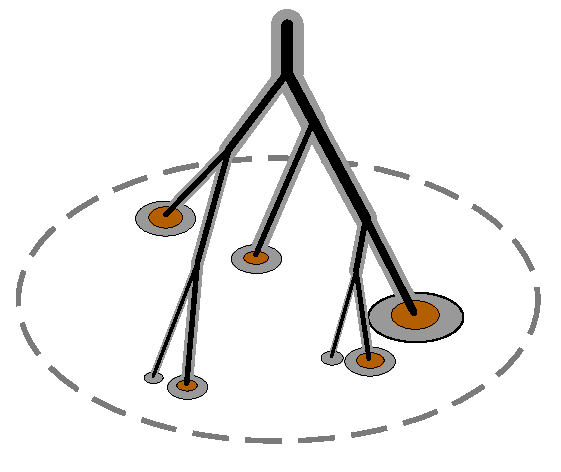
\includegraphics[width=.4\textwidth]{figures/piranha/cartoons/RSF_half_vis.pdf}
          };
          % \node at (0, 3.3) {Visualization of \normalsize \PRSF{1/2} (Balanced P-RSF)};
          % \node at (0, 2.8) {acting on a toy event};
          \node at (0, 2.8) {\normalsize \PRSF{1/2} (Balanced P-RSF)};
      \end{tikzpicture}
      \label{fig:rsf_half_vis}
      }
      ~~~~
      \subfloat[]{
      \begin{tikzpicture}
          \node at (0,0) {
              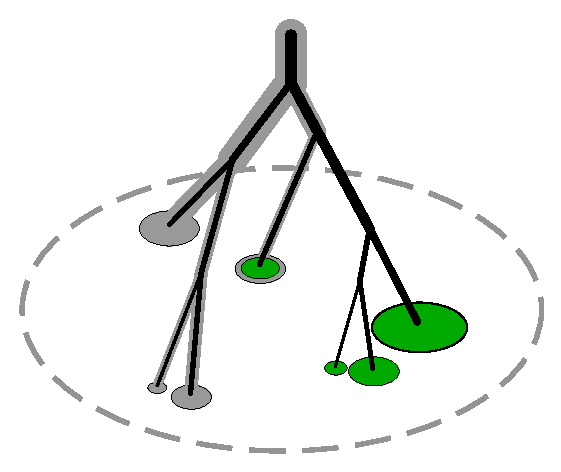
\includegraphics[width=.4\textwidth]{figures/piranha/cartoons/RSF_1_vis.pdf}
          };
          % \node at (0, 3.3) {Visualization of \normalsize \PRSF{1} (an example of};
          % \node at (0, 2.8) {Unbalanced P-RSF) acting on a toy event};
          \node at (0, 2.8) {\normalsize \PRSF{1} (example of Unbalanced P-RSF)};
      \end{tikzpicture}
      \label{fig:rsf_1_vis}
      }
      } % centerline
      \caption[Visualizations of recursive subtraction algorithms acting on toy jets.]{
    Visualization of (a) \PRSF{1/2} and (b) \PRSF{1} acting on a toy jet depicted as an angular-ordered tree of emissions.
    %
    The jet cone is indicated by the dashed ellipse, and the groomed final-state particles are indicated by colored ellipses, in dark orange (\PRSF{1/2}) and green (\PRSF{1});
    %
    the size of each circle is proportional to the groomed \(p_T\) of the corresponding particle.
    %
    The grey highlights behind each emission in the tree indicate the transverse momentum subtracted from each branch, and eventually from the final-state particles of that branch, as described in \Sec{recursive-subtraction}.
    %
    The size of the grey highlights behind each final-state particle indicates the amount of transverse momentum subtracted from that particle.
}
\label{fig:rsf_tree}
\end{figure}



%=====================================
% Continuity of P-RSF:
%=====================================
\gls{rsf} is well-defined on the space of energy distributions of particle events because it is invariant under exactly collinear splittings.
%
To see this, we first notice that exact collinear splittings are infinitely narrow, and always correspond to branchings at the final layer of an angular-ordered tree of emissions.
%
With this in mind, let us implement an exact collinear splitting, replacing a final-state particle \(i\) within a jet by two exactly collinear final-state particles, ``\(i,\,\text{soft}\)'' and ``\(i,\,\text{hard}\)''.
%
Following the presentation of \Sec{recursive-subtraction}, the transverse momentum subtracted from the new final state particles adds up to the transverse momentum subtracted from \(i\), \(\Delta^{(i,\,\text{soft})} + \Delta^{(i,\,\text{hard})} = \Delta^{(i)}\).
%
Since \(i,\,\text{soft}\) and \(i,\,\text{hard}\) are exactly collinear, the energy distribution of \(i\) after grooming is equal to the sum of the energy distributions for \(i,\,\text{soft}\) and \(i,\,\text{hard}\) after grooming.
%
The result of the \gls{rsf} grooming procedure is therefore robust against exactly collinear splittings for any value of \(f_{\rm soft}\).

While the subtractive algorithm of \gls{rsf} cannot be expressed simply in terms of geometry, \gls{rsf} echoes the features of \gls{apollonius} and \gls{ivs} that grant their continuity.
%
For example, Steps 3(a) and 3(b)
%Steps~\ref{item:remove_soft} and~\ref{item:remove_hard}
of the \gls{rsf} algorithm ensure that \gls{rsf} does not assign an area to any final-state particle that is larger than its transverse momentum.

However, \gls{rsf} still suffers from discontinuities in suppressed regions of parameter space.
%
We show in \Sec{rsf_discont} that Unbalanced \gls{rsf}, or \gls{rsf} with \(f_{\rm soft} \neq 1/2\), suffers from soft discontinuities:
%
small changes to the energy of the jet have the potential to change which emissions of the jet are softer.
%
The balanced recursive subtraction procedure, \PRSF{1/2}, overcomes this weakness and is soft-continuous.
%
Furthermore, \Sec{ang_discont} discusses how recursive tree-based grooming algorithms suffer from discontinuities inherited from pairwise clustering, leading to angular discontinuities in both Balanced and Unbalanced \gls{rsf} as well as traditional grooming algorithms such as Soft Drop.


%=====================================
% EMD:
%=====================================
\subsection{The Energy Mover's Distance and Precise Notions of Continuity}
\label{sec:emd}

We now prepare for a precise definition of continuity, and therefore a precise characterization of the continuity properties of \PIRANHA{} groomers.
%
\Gls{continuity} roughly means that small changes in the input to a function only lead to small changes to the output of the function.
%
Therefore, to define continuity, we will need to define what is meant by a ``small change'' in the final state of a particle collision event.

The tool we will use to understand when two particle collision events are similar is the \textit{Energy Movers' Distance} of Ref.~\cite{Komiske:2019fks}, which provides a quantitative measure of the similarity between two jets.
%
We introduce the EMD here both to facilitate our definition of continuity in jet grooming and as a useful tool for quantifying the responses of jet groomers to low-energy pollution.

%%
%Here and in the remainder of the paper, we borrow the terminology of \Reff{Komiske:2020qhg} and use the terms ``event'' and ``collider event'' to refer to the \textit{energy flow} of the event, or the angular distribution of energy of its outgoing radiation (as in \Def{energy-flow}).



\begin{definitionbox}{Energy Mover's Distance (EMD)}{emd}
    The EMD is a metric on the space of collider events which may be thought of as the amount of ``work'' required to rearrange one event into another.

    \vspace{7pt}
    \hrule
    \vspace{7pt}

    For events that consist of a finite number of outgoing particles, the \vocab{Energy Movers' Distance (EMD)} is defined as the solution to the optimal transport problem
    \begin{equation}
        \label{eq:EMD_def_1}
        {\rm EMD}_{\beta, R}\left(\mathcal{E}, \mathcal{E}'\right)
        =
        \min_{f_{ij} > 0} \sum_{i = 1}^M \sum_{j = 1}^{M'} f_{ij} \left(\frac{\theta_{ij}}{R}\right)^\beta
        +
        \left| \sum_{i = 1}^M E_i -  \sum_{j = 1}^{M'} E'_j\right|,
    \end{equation}
    \begin{equation}
        \sum_{i = 1}^M f_{ij} \leq E_j',
        ~~
        \sum_{j = 1}^{M'} f_{ij} \leq E_i,
        ~~
        \sum_{i = 1}^M \sum_{j = 1}^{M'} f_{ij}
        = \min\left(\sum_{i = 1}^M E_i, \sum_{j = 1}^{M'} E'_j\right)
        \label{eq:EMD_def_2}
        ,
    \end{equation}
    where \(i \in \{1, ..., M\}\) indicates a final-state particle of \(\mathcal{E}\) with energy \(E_i\), \(j \in \{1, ..., M'\}\) indicates a final-state particle of \(\mathcal{E}'\) with energy \(E'_j\), and \(\theta_{ij}\) denotes an angular distance between particles \(i\) and \(j\).
    %
    \(\beta > 0\) and \(R > 0\) are free parameters that control the behavior and relative importance of the first term on the right-hand side of \Eq{EMD_def_1}.\footnote{
    Strictly speaking, the EMD defines a metric only if \(2 R\) is greater than the maximum possible angular distance \(\theta_{ij}\).
    %
    Furthermore, for \(\beta > 1\), one must raise the first term of \Eq{EMD_def_1} to the \(1/\beta\) power.
    %
    We use the EMD without a subscript, \(
    {\rm EMD}\left(\mathcal{E}, \mathcal{E}'\right)
    \) to denote the EMD with \(\beta = 1\) and with large enough \(R\) that it furnishes a metric.
    }
\end{definitionbox}


We adopt the hadronic angular measure of \Reff{Komiske:2020qhg}, given by
\begin{equation}
    \theta_{ij} = \sqrt{-(n_i - n_j)^2}
    ,
    ~~~~~~
    ~~~~~~
    n_{i}^\mu = \frac{p_i^\mu}{E_{T\,i}} = (\cosh(y_i), \textbf{v}_{T\,i}, \sinh(y_i))^\mu
    .
    \label{eq:hadronic_metric}
\end{equation}
Here, \(n_i^\mu\) is a vector describing the motion of particle \(i\), parametrized by its rapidity \(y_i\) and its velocity \(\textbf{v}_{T\, i}\) in the directions transverse to the beampipe.
%
This angular metric reproduces the rapidity-azimuth distance between particles \(i\) and \(j\) in the small rapidity-azimuth distance limit.\footnote{
Another popular choice for the form of the \(n_i^\mu\) is captured by
\begin{align}
    \label{eq:ee_metric}
    n_{i,~{e^+e^-}}^\mu = \frac{p_i^\mu}{E_i} = (1, \textbf{v}_i)^\mu
    ,
\end{align}
which is a natural choice in the study of electron-positron collisions~\cite{Komiske:2020qhg}.
%
This choice reproduces the real-space opening angle between particles \(i\) and \(j\) in the small angle limit.
}

The EMD between a groomed jet in the presence and absence of low-energy pollution also provides an observable-independent tool for quantifying the sensitivity of jet grooming to pollution from \glspl{soft-distortion} and \gls{additive-contamination}.
%
Since the EMD furnishes a metric on the space of events, two events are separated by zero EMD iff they have identical energy flow, and two jets separated by zero EMD will yield the same value for every infra-red/collinear (IRC) safe observable (see \href{https://arxiv.org/pdf/2004.04159.pdf#page=11\&zoom=100,0,650}{Lemma 1} of \Reff{Komiske:2020qhg}).
%
Further, the EMD between two events also \textit{directly} bounds the differences in a large class of IRC-safe observable quantities (Lipschitz continuous observables) between the events~\cite{Komiske:2019fks}.
%
For example, the EMD between a parton-level jet and the same jet after \gls{hadronization} (the parton-hadron EMD) directly bounds the difference between a large class of parton- and hadron-level IRC-safe observables.
%
The parton-hadron EMD is therefore a powerful, observable independent tool for characterizing the response of a jet to \glspl{soft-distortion} from \gls{hadronization}.
%
We use the EMD in our analysis of grooming sensitivity to several sources of low-energy pollution in \Secs{soft_distortion}{add_contam}.


We may use the EMD to define continuity more precisely for maps on energy flows, in the spirit of \href{https://arxiv.org/pdf/2004.04159.pdf#page=5\&zoom=100,0,350}{Definition 1} of \Reff{Komiske:2020qhg}:
%
\begin{definitionbox}{Continuity at an Event}{eventcontinuity}
    \emph{\glslink{eventcontinuity}{continuous at an event}}

    \vspace{7pt}
    \hrule
    \vspace{7pt}

    A map \(M\) from energy flows to energy flows is \vocab{continuous at an event \(\mathcal E\)} if, for any \(\varepsilon > 0\), there exists a \(\delta > 0\) such that for all \(\mathcal E'\),
    %
    \begin{equation*}\label{eq:emdcontinuity}
        {\rm EMD}(\mathcal E,\mathcal E')<\delta
        \quad\implies\quad
        {\rm EMD}(M(\mathcal E), M(\mathcal E')) < \varepsilon.
    \end{equation*}
    %
    We say that \(M\) is \textbf{continuous} if it is continuous at all events \(\mathcal{E}\).
\end{definitionbox}
%
\noindent Definition~\ref{def:eventcontinuity} encodes the requirement that a continuous grooming algorithm must map jets that are infinitesimally nearby in event space to groomed results that are also infinitesimally close.\footnote{
%Our Definition~\ref{def:eventcontinuity} is in the spirit of \href{https://arxiv.org/pdf/2004.04159.pdf\#page=5\&zoom=100,114,645}{Definition 1} of \Reff{Komiske:2020qhg}.
Equivalently, we may say that a grooming procedure is continuous if it maps nearby jets to nearby groomed jets.
%
An event \(\mathcal{E}\) is \textbf{near} an open ball \(\mathcal{B}\) if any neighborhood of \(\mathcal{E}\) contains events in \(\mathcal{B}\).
%
On the real line, for example, the point \(E = 1\) is near the open ball \(B = (-1, 1)\).
%
A grooming procedure \(G\) is then \textbf{continuous} if for any event \(\mathcal{E}\) and open ball \(\mathcal{B}\),
%\begin{equation*}
    \(
    \mathcal{E} {\text ~is~ near~} \mathcal{B}
    \implies
    G(\mathcal{E}) {\text~ is~ near~} G(\mathcal{B}).
    \)
%\end{equation*}
}
For the more complicated \PIRANHA{} groomers we introduce in this paper, it will be helpful to define two additional properties that are required by full continuity:
\begin{itemize}
    \item
        \glslink{soft-discontinuity}{\vocab{Soft Continuity}} is the requirement that a groomer is invariant under infinitesimally soft perturbations of the energies of jet constituents;

    \item
        \glslink{angular-discontinuity}{\vocab{Angular Continuity}} is the requirement that a groomer is invariant under infinitesimally small angular changes in the directions of jet constituents.
\end{itemize}
\sam{Maybe this belongs earlier}

We will see that hard-cutoff groomers and even many recursive subtraction algorithms suffer from soft discontinuity in \Secs{softdrop}{rsf_discont} respectively.
%
In \Sec{ang_discont}, we will explore how tree-based grooming algorithms -- hard-cutoff and \PIRANHA{} alike -- may inherit angularly discontinuous behavior from angular-ordered jet clustering.\footnote{
Collinear safety, or invariance under exact collinear splittings which replace a final-state particle of momentum \(p^\mu\) by two particles with momenta \(\lambda p^\mu\) and \((1-\lambda) p^\mu\), is a weaker condition.
%
Exact collinear splittings do not change the energy distribution associated with an event; therefore, any well-defined map on the space of particle events must be collinear safe~\cite{Komiske:2020qhg}.
}



%=====================================
% The PIRANHA Paradigm for Jet Grooming:
%=====================================
\subsection[Back to School: Fully Continuous \textsc{Piranha} Grooming]{Back to School: Fully Continuous PIRANHA Grooming}
\label{sec:fully-continuous-piranha}

\PIRANHA{} grooming may be intuitively imagined as the optimal transport of a group of hungry piranhas towards the low-energy pollution within a jet.
%
In this analogy, henceforth the piranha analogy, a \PIRANHA{} groomer populates the \(\eta\)-\(\phi\) plane with a school of piranhas, distributed according to a particular model of the polluting energy density.
%
When they are given an event to groom, the piranhas discuss which piranhas will get to eat which jet constituent;
%
in the language of optimal transport, we say that the piranhas decide on a set of transport plans.
%
The piranhas then implement the plan and feed on the constituents of the jet, or subtract from the \(p_T\) of each jet constituent.
%
%\PIRANHA{} grooming uses optimal transport to design \textit{continuous} grooming procedures that have reduced sensitivity to low-energy pollution.
%%
%In particular, continuity requires that minuscule changes to the jet do not dramatically change the resulting groomed jet.
%
In the piranha analogy, continuity emerges when the piranhas' transport plans do not respond dramatically to small changes in the constituents of an ungroomed jet.
%
Since both \glspl{soft-distortion} and fluctuations in \gls{additive-contamination} may lead to small changes in an event, continuity helps ensure that neither dramatically changes the information carried by groomed jets.


The EMD itself also furnishes an example of an optimal transport problem, allowing us to immediately introduce a simple, generic \PIRANHA{} groomer.
%
To begin, let us model the radiation that we would like to remove from our jet as a distribution of energy \(\rhoC\) in a portion of the rapidity-azimuth (\(\eta\)-\(\phi\)) plane with area \(A\).
%
We use \(\rho\) to indicate the mean energy density and \(\mathcal{C}\) to indicate a distribution modeling the shape of the contaminating radiation, normalized such that
\begin{equation}
    \rho\int \dd y\,\dd\phi\,\mathcal{C}(y,\phi) = \rho A = E
\end{equation}
gives the total energy of the \gls{additive-contamination} we would like to remove.
%
Again echoing \Reff{Komiske:2020qhg}, we may phrase the subtraction of the energy distribution \(\rhoC\) from an event \(\mathcal{E}\) as the solution to the optimal transport problem
\begin{align}
    \label{eq:simple_piranha}
    \mathcal{E}_g[\mathcal E_0] = \underset{\mathcal{E}'}{\arg \min}\ {\rm EMD}_{\beta, R}
    \left(\mathcal{E}_0, \mathcal{E}' + \rhoC\right)
    .
\end{align}
%
It was shown in \href{https://arxiv.org/pdf/2004.04159.pdf#page=33\&zoom=100,0,0}{Lemma 3} of \Reff{Komiske:2020qhg} that \Eq{simple_piranha} defines a subtractive algorithm that merely decreases the energy of jet constituents, and does not add new particles to an event.
%
In the piranha analogy, \(\rhoC\) roughly describes the distribution of our piranhas, with a ``piranha energy density'' \(\rho\), while the minimization problem of \Eq{simple_piranha} provides them with the transport plans that guide them to subtract from the \(p_T\) of jet constituents.
%
Furthermore, the form of \(\mathcal{E}_g[\mathcal E_0]\) in \Eq{simple_piranha} is manifestly continuous due to its dependence on the EMD metric.%
\footnote{
    While \(\mathcal{E}_g[\mathcal E_0]\) in \Eq{simple_piranha} is continuous, manifest continuity due to dependence on the EMD should be treated skeptically.
    %
    For example, the ``grooming procedure'' associated with  \Eq{simple_piranha} may not be continuous if the \(\arg \min\) operation is restricted to a non-convex sub-space of the full space of events.
    %
    Analogously, \(
        f(x)
        =
        \underset{y}{\arg \min}\ ||x, y+1||
        =
        x-1
    \)
    is continuous as a map from \(\mathbb R\) to \(\mathbb R\) with the standard topology.
    %
    However, \(
        g(x)
        =
        \underset{y \in \{0, 1\}}{\arg \min}\ ||x, y+1||,
    \)
    which differs only by the allowed values of \(y\) in the \(\arg \min\), is not.
}



%-----------------------------------
% Apollonius fig.:
%-----------------------------------
\begin{figure}[t!]
\centering

\subfloat[%\normalsize Visualizing the \PIRANHA{} Paradigm
]{
\begin{tikzpicture}
\node at (0,0) {
    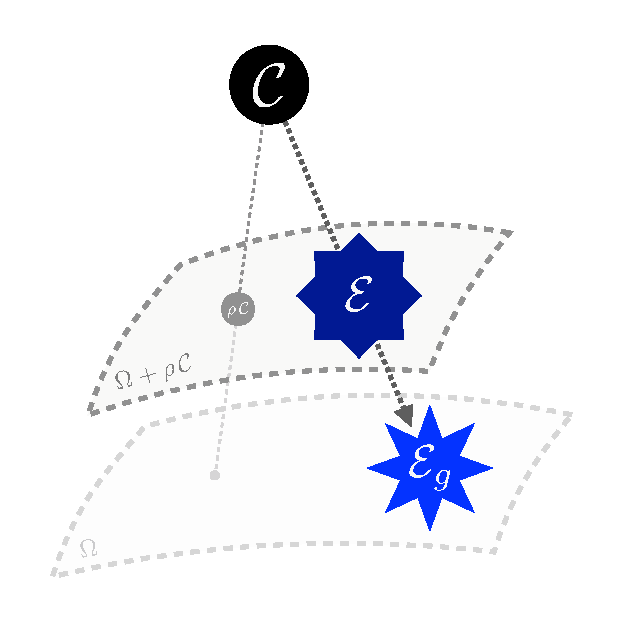
\includegraphics[width=0.45\textwidth]{figures/piranha/cartoons/space_pu}
};
\node at (0,4.25) {Cartoon of a \PIRANHA{} groomer};
\node at (0,3.75) {acting on the space of energy flows};
\end{tikzpicture}
\label{fig:piranha_projection}
}
\subfloat[%\normalsize Apollonius Subtraction
]{
\begin{tikzpicture}
\node at (0,0) {
\includegraphics[width=0.45\textwidth]{figures/piranha/event_visualizations/apollonius_diagram_pink}
};
\node at (0,4.35) {Visualization of \gls{apollonius} acting on};
%\node at (0,4.25) {P-AS Acting on an Example Event};
\node at (0,3.85) {an event generated in \texttt{Pythia 8.244}};
\end{tikzpicture}
\label{fig:apollonius_subtraction}
}
\caption[Cartoons depicting implementations of the \textsc{Piranha} paradigm, based on a figures from \Reff{Komiske:2020qhg}.]{
    (a) A cartoon of a generic implementation of the \PIRANHA{} paradigm described by \Eq{simple_piranha}, based on a figure from \Reff{Komiske:2020qhg}.
    %
    \(\mathcal{E} \in \Omega\) indicates a particular event \(\mathcal{E}\) in the space \(\Omega\) of events to be groomed, \(\mathcal{C}\) indicates a model energy distribution for contaminating radiation, and \(\rho\in \mathbb{R}\) parametrizes the strength of the grooming.
    %
    \Eq{simple_piranha} uses these ingredients to produce the groomed event \(\mathcal{E}_g\).
    %
    (b) An Apollonius diagram in the rapidity-azimuth plane, also from \Reff{Komiske:2020qhg}, used by the \glslink{apollonius}{Apollonius Subtraction (P-AS) algorithm}.
    %
    \gls{apollonius}, an implementation of the \PIRANHA{} paradigm described in \Sec{as}, models contaminating radiation as uniform in the rapidity-azimuth plane \(\mathcal C = \mathcal U\).
    %
    The color intensity of each Apollonius region is proportional to the amount by which the corresponding particle \(i\) is groomed, and thus to the area \(A^{\rm Apoll.}_i\) of the region.
}
\label{fig:as}
\end{figure}


%---------------------------------------------------------------------
% Apollonius:
%---------------------------------------------------------------------

\glslink{apollonius}{Apollonius Subtraction (P-AS)} is a direct application of \Eq{simple_piranha} in which we take contaminating radiation to be uniformly distributed in a region of the \(\eta\)-\(\phi\) plane bounded by a maximum pseudorapidity, \(|\eta| < \eta_{\rm max}\).
%
We denote the uniform event with energy density \(\rho\) by \(\rhoU\).
%
This has proven to be an effective model for \glslink{pileup}{pileup}, \glslink{ue}{the underlying event}, and initial state radiation~\cite{Soyez:2018opl,Monk:2018clo,Sjostrand:1987su,Sjostrand:2014zea,Dasgupta:2007wa,Kirchgaesser:2020poq,Moraes:2007rq,CDF:2015txs,Larkoski:2021hee,Baron:2020xoi,Marzani:2017kqd}, and was the original motivation for the \PIRANHA{} approach to continuous jet grooming outlined in this chapter.

\begin{definitionbox}{Apollonius Subtraction (P-AS)}{apollonius}
    \glslink{apollonius}{\vocab{Apollonius Subtraction (P-AS)}} is a \PIRANHA{} groomer defined directly as the solution to the optimal transport problem
\begin{align}
    \label{eq:apollonius-definition}
    \mathcal{E}_g[\mathcal E_0] = \underset{\mathcal{E}'}{\arg \min}\ {\rm EMD}_{\beta, R}
    \left(\mathcal{E}_0, \mathcal{E}' + \rhoU\right)
    \,.
\end{align}

    \vspace{7pt}
    \hrule
    \vspace{7pt}

    More precisely, using \(\beta = 1\), \(R =1\), and replacing \(\rhoC\) with \(\rhoU\) in \Eq{simple_piranha} yields an optimal transport problem known as an \textit{Apollonius problem}.
    %
    The Apollonius problem is well studied in the optimal transport literature and can be solved with an \textit{Apollonius diagram}, or additively weighted Voronoi diagram, which assigns an \textit{Apollonius region} to each particle in the event.

    \gls{apollonius} may then be phrased as a constituent-level area subtraction procedure that solves the Apollonius problem for a given event.
    %
    To solve the Apollonius problem associated with a particular Apollonius diagram, we subtract from the \(p_T\) of each particle an amount proportional to the area of its Apollonius region,
    \(p_{T\,i}^{\rm AS} = p_{T\,i} - \rho A_i^{\rm Apoll.}\).
    %
    Letting \(\zcut = \rho \, A_{\rm tot} / p_{T\,{\rm tot}}\), in analogy to the \(\zcut\) of traditional groomers such as Soft Drop, we may equivalently write
    \(p_{T\,i}^{\rm AS} = p_{T\,i} - \zcut\,p_{T\,{\rm tot}}\,A_i^{\rm Apoll.} / A_{\rm tot}\).
    %
    In the piranha analogy, the transport plans for an event are determined by its Apollonius diagram, and all of the piranhas within a given Apollonius region feed on the associated jet constituent.
\end{definitionbox}

The precise structure of the Apollonius diagram corresponding to an event is described in a physics context in Section 5.4 of \Reff{Komiske:2020qhg}, and in the context of optimal transport in \Reffs{hartmann2017geometrybased,hartmann2018semidiscrete,bourne2018semidiscrete}.%
\footnote{
    \Eq{simple_piranha} with \(\rhoC = \rhoU\) and arbitrary positive \(\beta\) also describes a valid optimal transport problem and an associated \PIRANHA{} groomer.
    %
    The solution to the associated optimal transport problem is described by a \textit{generalized Laguerre diagram}~\cite{Komiske:2020qhg, bourne2018semidiscrete}.
    %
    We leave the study of \PIRANHA{} grooming motivated by generalized Laguerre diagrams for future work.
}
%
A rigorous proof of the continuity of \gls{apollonius} is given in \href{https://arxiv.org/pdf/1706.07403.pdf#page=15&zoom=100,0,200}{Lemma 3.3} of \Reff{hartmann2017geometrybased}, and a visual representation of \gls{apollonius}, taken from \Reff{Komiske:2020qhg}, is depicted in \Fig{as}.

%-----------------------------------
% Apollonius comparison:
%-----------------------------------
\gls{apollonius} is closely related to constituent-level area subtraction techniques for \gls{pu-mitigation}.
%
Indeed, \gls{apollonius} was initially introduced in the context of \gls{pu-mitigation} in \Reff{Komiske:2020qhg}, where it was shown that in certain limits, Apollonius Subtraction aligns with the discontinuous Voronoi Area Subtraction (VAS) procedure for \gls{pu-mitigation}~\cite{Cacciari:2007fd, Cacciari:2008gn, Cacciari:2011ma}.
%
Thus, \gls{apollonius} may be thought of as a continuous analog to existing techniques for constituent-level area subtraction.
%
\gls{apollonius} also aligns in certain limits with continuum Constituent Subtraction (CS), a continuous but computationally expensive algorithm for the removal of \glslink{pileup}{pileup}~\cite{Berta:2014eza, Komiske:2020qhg}.

Unfortunately, the computational cost of finding the Apollonius diagram for a given particle event is relatively high because we rely on directly solving the Apollonius problem using numerical ghosts~\cite{Komiske:2020qhg}:
%
we use a uniform grid of ``ghost'' particles in the \(\eta\)-\(\phi\) plane to obtain the Apollonius diagram associated with a particular event computationally.
%
Data collection and analysis for theoretical and experimental studies at colliders motivate the computationally efficient analogs of \gls{apollonius} that we describe in the remainder of this section.\footnote{Another approach to developing analogs of \gls{apollonius} that we do not pursue in this thesis is to use the formalism of \textit{linearized optimal transport}, explored mathematically in \Reffs{cai2022linearized,sarrazin2023linearized} and applied to particle collisions in \Reffs{Cai:2020vzx,Cai:2021hnn}, which preserves the strengths of the EMD and significantly reduces the computational costs associated with optimal transport problems.}
%
A comparison of the runtime for our different \PIRANHA{} algorithms is given in \Fig{runtimes} of \App{feedingfrenzy}.

%----------------------------------------------------------------------
% Iterated Voronoi:
%----------------------------------------------------------------------


\glslink{ivs}{Iterated Voronoi Subtraction (P-IVS)} is a \PIRANHA{} groomer similar to both \gls{apollonius} and VAS that overcomes the computational inefficiency of \gls{apollonius}.
%
\gls{ivs} also uses the uniform event \(\rho\,\mathcal U\) as a model for \gls{additive-contamination}, but crucially uses Voronoi diagrams rather than Apollonius diagrams to subtract this contamination away.

\begin{definitionbox}{Iterated Voronoi Subtraction (P-IVS)}{ivs}
    \glslink{ivs}{\vocab{Iterated Voronoi Subtraction (P-AS)}} is a grooming algorithm defined by a sequence of optimal transport problems which are more efficient to solve than the Apollonius problem.
    %
    Like \gls{apollonius}, the amount of grooming performed by the \gls{ivs} grooming procedure is encoded in a parameter \(\rho\).
    %
    We may describe \gls{ivs} quite succinctly as the solution to the iterated series of optimal transport problems~\cite{Komiske:2020qhg}:
    \begin{align}
        \mathcal{E}^{(n+1)}_{\rm IVS}
        =
        \underset{\mathcal{E}'}{\arg \min} ~ {\rm EMD}
        (\mathcal{E}^{(n)}, \mathcal{E}' + \rho^{(n)}\,\mathcal{U})
        \label{eq:ivs1}
        ,
    \end{align}
    with
    \begin{align}
        \rho^{(n)} =
        \min\left\{
            \rho - \sum_{i=0}^{n-1}\rho^{(i)},
        ~
        \min_i \frac{p^{(n)}_{T\,i}}{A^{(n)}_i}
        \right\}
        \label{eq:ivs2}
        .
    \end{align}
    %
    The final groomed event is given by the limit of the recursive procedure in \Eq{ivs1}, \(\mathcal{E}_{\rm IVS} = \lim_{n\to\infty} \mathcal{E}^{(n)}_{\rm IVS}\).
    %
    Here, \(\rho^{(0)} = 0\), \(p_{T\,i}^{(n)}\) is the transverse momentum of particle \(i\) after \(n\) applications of the recursive algorithm in \Eq{ivs1}, and \(A_i^{(n)}\) is the Voronoi region for the event after \(n\) applications of \Eq{ivs1}.
    %
    For example, \(p_{T\, i}^{(0)}\) and \(A_i^{(0)}\) describe the transverse momenta and Voronoi areas of the ungroomed event.

    \vspace{7pt}
    \hrule
    \vspace{7pt}

    More concretely, we may describe our ungroomed event as a collection of points in the \(\eta\)-\(\phi\) plane describing the directions of outgoing momenta, each weighted by its transverse momentum.
    %
    We may then enumerate the steps of the IVS procedure as follows:
    %
    \begin{enumerate}
        \item
        \gls{ivs} constructs a Voronoi diagram in the \(\eta\)-\(\phi\) plane for the particles in the event.
        %
        We will label the stage of the \gls{ivs} procedure by an integer \(n\), starting at \(n = 1\) and going up to at most the number of particles in the event.
        \label{enum:ivs_1}

        \item
        \gls{ivs} modifies the \(p_T\) of every particle in the event, subtracting \(p_T\) proportional to the area of the particle's Voronoi region until a particle would be removed or the grooming is complete:
        \begin{align}
        \label{eq:ivs_2}
        p_{T\,i}^{(n)} = p_{T\,i}^{(n-1)} - \rho^{(n)} A^{(n-1)}_i,
        \end{align}
        with \(\rho^{(n)}\) given by \Eq{ivs2}.
        \label{enum:ivs_2}

        \item
        If \(\rho - \sum_{i = 1}^n \rho^{(i)} > 0\), \gls{ivs} increments \(n\) by 1 and continues from Step~\ref{enum:ivs_1} by drawing a new Voronoi diagram for the modified event with a particle removed.
        %
        Otherwise, the grooming is complete.
        \label{enum:ivs_3}
    \end{enumerate}

\end{definitionbox}


As with \gls{apollonius}, the simple expression of \gls{ivs} in terms of the EMD already showcases its continuity and connection to optimal transport.
%
One may worry that the presence of an infinitesimally soft particle in an event may dramatically change the Voronoi diagram for an event, and therefore dramatically change the result of grooming using Voronoi areas.
%
\gls{ivs} overcomes this challenge by only using Voronoi areas until a particle is removed;
%
when a particle is removed from the event, \gls{ivs} computes an updated set of Voronoi areas that do not rely on the removed particle, continuing recursively until it has removed the correct amount of energy.
%
A rigorous proof of the continuity of \gls{ivs} is given in \href{https://arxiv.org/pdf/1706.07403.pdf#page=15&zoom=100,0,200}{Lemma 3.3} of \Reff{hartmann2017geometrybased}.


\remark{}{
    Unweighted Voronoi diagrams for the original event \(\mathcal{E}^{(0)}\) can be found efficiently, unlike the weighted Voronoi/Apollonius diagrams needed for \gls{apollonius}.
    %
    Furthermore, the Voronoi diagrams for the subtracted events \(\mathcal{E}^{(n)}_{\rm IVS}\) used throughout the stages of the \gls{ivs} algorithm do not need to be computed from scratch, and can be found in constant (amortized) time~\cite{Komiske:2020qhg}.
    %
    \gls{ivs} thus retains the continuous grooming properties of \gls{apollonius} while remaining amenable to numerical computation and data collection.
}

%-----------------------------------------------------
\subsection{Stronger Notions of Continuity}
%-----------------------------------------------------
\label{sec:stronger-continuity}

As a final note for this section, we point out that there are analogs of continuity that provide stronger constraints.
%
One example of a stronger form of continuity is \textit{uniform continuity}:
\begin{definitionbox}{Uniform Continuity}{uniform-continuity}
    A map \(M\) from energy flows to energy flows is \glslink{uniform-continuity}{\vocab{uniformly continuous}} if, for any \(\varepsilon > 0\), there exists a \(\delta > 0\) such that for all \(\mathcal{E}\) and \(\mathcal E'\),
    %
    \begin{equation*}
        \label{eq:emduniformcontinuity}
        {\rm EMD}(\mathcal E,\mathcal E') < \delta
        \quad\implies\quad
        {\rm EMD}(M(\mathcal E), M(\mathcal E')) < \varepsilon.
    \end{equation*}
    %
    Roughly, we might say that uniform continuity requires that when we pick \(\varepsilon\), \(M\) must be ``continuous with the same \(\delta\) for every event''.
\end{definitionbox}

\noindent
An even stronger condition is that of \textit{H\"older continuity}:

\begin{definitionbox}{H\"older Continuity}{holdercontinuity}
    A map \(M\) from energy flows to energy flows is \vocab{H\"older continuous} with exponent \(\alpha \in \mathbb R\) if, for all \(\mathcal{E}\) and \(\mathcal E'\),
    %
    \begin{equation*}\label{eq:emdholdercontinuity}
        {\rm EMD}(M(\mathcal E), M(\mathcal E'))
        <
        K \cdot \big({\rm EMD}(\mathcal E, \mathcal E')\big)^\alpha,
    \end{equation*}
    with \(K\in \mathbb R\) a constant.
    %
    The special case \(\alpha = 1\) is called \vocab{Lipschitz continuity}.
\end{definitionbox}

Placing stronger constraints on grooming, such as uniform continuity and H\"older continuity, has the potential to further constrain the effects of soft contamination and fluctuations in additive radiation on groomed results.
%
For example, in which regions of parameter space are the hard-cutoff or \PIRANHA{} groomers presented in this thesis uniformly or H\"older continuous?
%
Are other methods for continuous grooming, such as EMD-mode \PIRANHA{} introduced in \App{grooming_in_emd_mode} or \PIRANHA{} groomers designed using linearized optimal transport \cite{Cai:2020vzx,Cai:2021hnn,cai2022linearized,sarrazin2023linearized}, more amenable to strongly continuous generalizations?
%
Can this knowledge help us identify obstacles to achieving these stronger types of continuity and guide us in designing more powerful, robust observables and groomers?

Though we do not investigate grooming methods that utilize these more restrictive analogs of continuity in this thesis, the invention and understanding of such groomers offer an intriguing and promising avenue for future research.
%
Instead, the remainder of this chapter is devoted to introducing hard-cutoff grooming, examining the types of discontinuities that may emerge in jet grooming, and studying the sensitivity of the continuous groomers we introduced in this section to important examples of low-energy pollution that appear in the study of particle collision data.




%==============================================
\subsection[Resummed Recursive Subtraction]{Resummed Recursive Subtraction}
%==============================================
\label{sec:pira-resummed}


We would like to gain theoretical insight, where possible, into the properties of \PIRANHA{}-groomed jets.
%
To move towards a perturbative understanding of \PIRANHA{}, we begin by studying the behavior of \gls{rsf} at leading order (LO), deriving the results for \gls{rsf} substructure presented in \Sec{sd_discont_lo}, and describe why this is sufficient for generic \PIRANHA{} groomers at \glslink{accuracy}{NLO}.
%
Beyond \glslink{accuracy}{NLO}, we find difficulties in using existing resummation techniques because of the intricate correlations between subtractions of different emissions.
%
Nonetheless, we can study the specific example of \PRSF{1} to obtain analytic resummed results up to leading logarithmic accuracy (LL) and numerical results beyond LL.


We focus on quantifying the substructure of \PIRANHA{}-groomed jets using the two-prong generalized energy correlation functions (ECFs) of \Reff{Larkoski:2013eya}.
%
These were described by \Eqs{GECFdefn_lo}{ECFdefn_pheno}, and we repeat their approximate form in the central (\(y=0\)) and narrow (\(R_0 \ll 1\)) limit here for convenience:
\begin{equation}
    C_1^{(\varsigma)} \simeq \frac{1}{2}\sum_{i=1}^M\sum_{j=1}^M z_i z_j \left(\frac{\theta_{ij}}{R_0}\right)^\varsigma
    \label{eq:ECFdefn_repeat}
    .
\end{equation}
As before, \(z_i\) indicates the energy fraction of particle \(i\), \(\theta_{ij}\) indicates the opening angle between particles \(i\) and \(j\), and \(R_0\) is the jet radius.

The \(C_1^{(\varsigma)}\) furnish a set of interesting but relatively simple observables to study in the context of \PIRANHA{}.
%
The behavior of the \PIRANHA{} groomed jet \(p_T\), for example, is relatively uninteresting:
%
since the \PIRANHA{} groomers discussed in this thesis (other than the toy example of the constant subtraction algorithm) operate by subtracting a fixed amount of transverse momentum
\begin{align}
    \Delta p_T = \zcut\,p_T = \rho\,A_{\rm jet}
    ,
\end{align}
the changes to the transverse momentum of a jet due to the \gls{rsf} grooming procedure are set trivially by the parameter \zcut{}.
%
However, as discussed in \Sec{sd_discont_lo}, refining calculations of observables involving the energy fraction \(z_g\) or angle \(r_g\) of the first emission to pass the grooming is a nuanced task that we will defer to future work.


We first discuss the \glslink{accuracy}{NLO} behavior of the distributions for \gls{rsf} groomed ECFs, with a brief discussion of the \glslink{accuracy}{NLO} behavior of \PIRANHA{} groomers in general.
%
We then discuss the behavior of \gls{rsf}\(_{1}\) groomed ECFs at resummed accuracy, comparing results obtained with \gls{pqcd}, leading logarithmic parton showers, and \texttt{Pythia 8.244}.
%
We use the technology of \glspl{substructure-diagram} for our calculations in \gls{pqcd} and compare our results to a numerical parton shower whose structure is the subjet of Problem~\ref{prob:parton-shower}.


Because each emission is suppressed by a factor of \(\alpha_s\), the behavior of the \gls{rsf} groomed ECFs of \Eq{ECFdefn_repeat}, away from \(C_1^{(\varsigma)} = 0\), is determined by the phase space distribution of two-parton jets whose particles survive the \gls{rsf} grooming procedure, up to corrections proportional to \(\alpha_s^2\).
%
If the two partons survive the grooming procedure, they can be described with the modified energy fractions
\begin{subequations}
\begin{align}
    z_{\rm soft}' &= z - f\,\zcut > 0,
    \\
    z_{\rm hard}' &= 1 - z - (1-f)\zcut > 0,
\end{align}
\end{subequations}
where \(z\) is the original energy fraction of the softer parton.
%
The \gls{rsf}-groomed jet ECF then takes the form
\begin{equation}
    C_1^{(\varsigma)}(z,\theta)
    =
    \left(z - f\,\zcut\right) \left(\frac{\theta}{R_0}\right)^\varsigma \frac{\left(1 - z - (1-f)\zcut\right)}{\left(1 - \zcut\right)^2}
    \approx
    \left(z - f\,\zcut\right)\left(\frac{\theta}{R_0}\right)^\varsigma
    \,
    \frac{\left(1 - (1-f)\zcut\right)}{\left(1 - \zcut\right)^2}
    \label{eq:oneEm_groomedECFdefn}
    .
\end{equation}
%
In the last step, we use that the phase space of the emission is dominated by regions with \(z,\,\theta \ll 1\).
%
The factors of \((1-\zcut)^2\) that appear in the denominators of \Eq{oneEm_groomedECFdefn} emerge from the normalization of the groomed \(C_1^{(\varsigma)}\) by the groomed jet \(p_T\), as in the definition of \Eq{ECFdefn_repeat}.

We also note that if either of the partons in our two-parton configuration at \glslink{accuracy}{NLO} is entirely groomed away, the groomed value of \(C_1^{(\varsigma)}\) is zero.
%
The region of phase space where one parton is groomed away at \glslink{accuracy}{NLO} conspires with virtual contributions and the one-parton configuration with no splittings to ensure that the \(C_1^{(\varsigma)}\) distribution integrates to one.
%
These contributions may quickly be calculated once we find the distribution away from the origin, \(C_1^{(\varsigma)} > 0\), and we include them at the end of the following discussion.


The \(C_1^{(\varsigma)}\) distribution of \gls{rsf}-groomed jets takes a similar form to that of \glslink{constant-subtraction}{constant-subtraction-groomed} jets, as in Example~\ref{ex:constant-subtraction-gecf}.
%
Concretely, the fixed-order distribution of \(C_1^{(\varsigma)}\) away from zero becomes
%
\begin{align}
    \rho^{\rm(LO)}_{i,~\varsigma}(C>0)
    =
    \frac{\alpha_s}{\pi}\int_0^{R_0}\frac{\dd\theta}{\theta}
    \int_0^{1/2} \dd z\, \Bar{p}_i(z)
    \delta\left(C - C_1^{(\varsigma)}(z,\theta)\right),
    \label{eq:LO_dist_setup}
\end{align}
%
where  \(C_1^{(\varsigma)}(z,\theta)\) is the functional form of the groomed ECF given in \Eq{oneEm_groomedECFdefn}.

\begin{exercise}
    \label{ex:rsf-gecf}
    Up to terms that are power-suppressed in \(C\), \(\zcut\), or both, show that the NLO distribution for \gls{rsf}-groomed \gls{gecf} away from \(C = 0\) is
    %
    \label{eq:prsf_LO}
    \begin{align}
        \rho^{\rm(LO)}_{i,~\varsigma}(C>0)
        &=
        \frac{2\alpha_s C_{R_i}}{\varsigma~\pi}
        \frac{1}{C}
        \left(
            2\tanh^{-1}\left(1  -2 \tilde C - 2\,f\,\zcut\right)
            + B_i
            +
            \mathcal{O}\left(C,\,\zcut\right)
        \right)
        \\
        &=
        \frac{2\alpha_s C_{R_i}}{\varsigma~\pi}
        \frac{1}{C}
        \left(
            -\log\left(\tilde C + f\,\zcut\right)
            + B_i
            +
            \mathcal{O}\left(C,\,\zcut\right)
        \right)
    \end{align}
    %
    where \(\tilde C = C \times (1-\zcut)^2 / (1 - (1-f)\zcut)\), \(C_{R_i}\) is the quadratic Casimir of the color representation of the initiating parton, and we have defined the factor \(B_i\) to capture behavior from non-singular components of the splitting functions:
    %
    \(B_q = -3/4\) for quark initiated jets and \(B_g = -11/12 + n_f/(6 C_A)\) for gluon initiated jets.
\end{exercise}

\remark{}{
    As in Exercise~\ref{ex:constant-subtraction-virtual}, including the \(\mathcal{O}(\alpha_s^0)\) jet configuration with a single parton for which \(C_1^{(\varsigma)} = 0\), the two-parton contributions for which \(z < f \zcut\) and the softer emission is completely eliminated, and the virtual contributions at \(\mathcal{O}(\alpha_s^1)\), we can write the full \glslink{accuracy}{NLO} probability distribution for \(C_1^{(\varsigma)}\) as
    \begin{align}
        \label{eq:plusdist_prsf_lo}
        \rho^{\rm(LO)}_{i,~\varsigma}(C)
        &\approx
        \delta(C)
        +
        \frac{2\alpha_s C_{R_i}}{\varsigma~\pi}
        \left[\frac{1}{C}
        \left(
            -\log\left(\tilde C + f\,\zcut\right)
            + B_i
            +
            \mathcal{O}\left(C,\,\zcut\right)
        \right)
        \right]^{(C_{\rm max})}_+
        ,
    \end{align}
where \({C_{\rm max}} = (1/2 - f \zcut)(1 - (1-f)\zcut)/(1 - \zcut)^2\) is the maximum value of \(C_1^{(\varsigma)}\), and we have fixed the normalization of the distribution with \glslink{plus-fn}{plus-function regularization}.
    %
    \Eq{plusdist_prsf_lo} can be obtained simply by using the same logic of \textit{sum rules} discussed in the hint to Exercise~\ref{ex:constant-subtraction-virtual}:
    %
    we need only remember that the full distribution for \(C_1^{(\varsigma)}\) must integrate to one even at \glslink{accuracy}{NLO}, and additional contributions to the \glslink{accuracy}{NLO} distribution in \Eq{prsf_LO} can only come from the regions of phase space where \(C_1^{(\varsigma)}=0\).
    %
    Like the NLO \glslink{constant-subtraction}{constant-subtraction-groomed} substructure distributions, and unlike the \glslink{accuracy}{NLO} distributions for traditionally groomed jet substructure, the \glslink{accuracy}{NLO} distributions for \gls{rsf} groomed \(C_1^{(\varsigma)}\) do not exhibit piece-wise behavior, providing a hint of the continuity of \gls{rsf}.
}



The global nature of \PIRANHA{} grooming algorithms leads to intricate correlations between the grooming of different final-state particles, and thus to complications in perturbative calculations beyond \glslink{accuracy}{NLO}.
%
For \PRSF{1/2}, \gls{ivs}, and \gls{apollonius}, every particle in a jet is groomed by some amount, and the grooming of any particular final-state particle is correlated with the grooming of every other.
%
This subtlety renders existing techniques for multiple emissions calculations less effective.
%
\PIRANHA{}-groomed observables depend on global information, and a more detailed understanding of \PIRANHA{}-groomed correlators will require techniques that can elucidate global information associated with a jet.

While we do not get around this subtlety for the \PIRANHA{} grooming procedures presented in this paper, we may use \gls{rsf} to at least gain some intuition for the resummed behavior of recursive subtractors.
%
In particular, we navigate around the subtleties associated with \PIRANHA{} by studying the substructure of \gls{rsf} with \(f_{\rm soft} = 1\), or \PRSF{1}.
%
Crucial to our analysis is that \PRSF{1} eventually terminates, such that it does not necessarily affect every particle within an event.\footnote{
\PRSF{0} is another subtraction algorithm that eventually terminates, but it subtracts away hard radiation instead of soft radiation.
%
Therefore, we focus on \PRSF{1} in the discussion below.
%
We leave a more detailed survey of the analytic properties of \PRSF{1/2}, \PRSF{0}, and Recursive Subtraction more generally to future work.
}
%
Due to this additional simplicity, we can study \PRSF{1} at leading logarithmic (LL) accuracy in slightly more detail, and find analytic expressions for observables related to the first emission to survive the grooming procedure, or the \gls{crit-emission}.


The properties of the groomed \gls{crit-emission} -- and in particular its energy fraction \(z_g\) -- were discussed in Remark~\ref{rem:soft-drop-zg}, which will provide a useful guide for our discussion of the \gls{crit-emission} of \gls{rsf}.
%
The behavior of the \gls{rsf} \(z_g\) distribution is more subtle than that of Soft Drop, for reasons we discuss below.
%
At the level of a single emission, however, the \(z_g\) distribution for Soft Drop may be translated directly to \gls{rsf} because of the similarities between Soft Drop with \(\beta = 0\) and \gls{rsf}.
%
Defining \gls{rsf}, \(z_g\) is the groomed energy fraction of the \gls{crit-emission} and translating the \gls{soft-drop} result gives%
\footnote{
    In \Eq{prsf_zg_lo}, we choose \(z_g\) to be the groomed energy fraction of what had been the softer emission before grooming, regardless of which emission is softer after grooming.
    %
    This avoids additional corrections if \(f_{\rm soft} < 1/2\), where more grooming is applied to the harder emission than the softer emission at each branch and it becomes possible that the harder of two ungroomed emissions becomes the softer of the two emissions after grooming.
    %
    If we instead define \(z_g\) to be the softer \textit{groomed} emission, there are corrections to this formula for \(z_g > 1/2 - \mathcal{O}(\zcut)\) when \(f_{\rm soft} < 1/2\).
    %
    We also assume that \(\zcut < 1/2\);
    %
    if \(f_{\rm soft} < 1/2\) and \(\zcut > 1/2\), there are additional \(\mathcal{O}(\zcut)\) corrections to \Eq{prsf_zg_lo} due to the constraint that the harder ungroomed emission is not entirely groomed away.
}
\begin{align}
    \rho_{i,\,\,\text{P-RSF}}(z_g; f)
    =
    (1-\zcut)
    \frac{
    \overline{p}_i\left[
        \left(1 - \zcut\right)z_g\,+\,f \zcut
    \right]
    }
    {\int_{f \zcut}^{1/2} \dd z' \,\, \overline{p}(z')}
    +
    \mathcal{O}(\alpha_s)
    \label{eq:prsf_zg_lo}
    .
\end{align}
\(\rho_{i,\,\,\text{P-RSF}}(z_g; f)\) has support in the domain \(z_g \in \left(0,\,(1/2 - f\zcut)\,/\,(1-\zcut)\right)\) at this order of accuracy.
%
The additional factors of \((1-\zcut)\) relative to \Eq{sd_zg} capture the fact that \(z_g\) is normalized further after grooming:
%
\(z_g = (z_0 - f\zcut)/(1-\zcut)\), where \(z_0\) denotes the ungroomed softer energy fraction.
%
The lower limit \(f \zcut\) on the integration variable \(z'\) reflects that we consider configurations for which the softer emission survives the grooming procedure.

Much like Soft Drop with \(\beta_{\rm SD} = 0\), the \glslink{accuracy}{NLO} behavior of the \gls{rsf} \(z_g\) distribution is determined by the fact that the first surviving emission must have an energy fraction greater than the assigned grooming.
%
At \glslink{accuracy}{NLO}, there is a single emission, and therefore the assigned grooming is simply \(f \zcut\).
%
Unlike Soft Drop, however, the \(z_g\) distribution for \gls{rsf} has support down to \(z_g = 0\):
%
a two-parton event with \(z = f \zcut + \delta\), \(\delta \ll 1\), is mapped to a groomed two-parton event with \(z_g = \delta\), while the two-parton event with \(z = f \zcut - \delta\) is mapped to a one-parton event;
%
though \(z_g\) is undefined in the latter case, where the groomed jet consists of only a single parton, the fact that \(z_g\) can become infinitesimally small is a mark of the continuity of \gls{rsf}.

Improving the accuracy of the calculation of \(z_g\) for \gls{rsf} will require a more detailed analysis which we leave to future work.
%
An important complication emerges because there may be emissions before the critical emission that can soak up some of the grooming;
%
the amount by which the critical emission is groomed is therefore not \(\zcut\) but a smaller effective value, \(\zcut^{\rm(eff)} = \zcut - \Delta \zcut\), where \(\Delta \zcut\) depends on the energy fractions of earlier emissions.
%
This leads to problems when following the approach of \Reff{Larkoski:2015lea}, suited to the calculation of \(z_g\) for Soft Drop.
%
\Reff{Larkoski:2015lea} calculates the distribution of \(z_g\) in the framework of Sudakov safety by first marginalizing over the distribution of the angle of the critical emission, \(r_g\).
%
However, the distribution of \(r_g\) depends on the amount by which the critical emission is groomed, \(\zcut^{(\rm eff)}\), while a leading logarithmic calculation of \(\zcut^{(\rm eff)}\) depends on the value of \(r_g\).
%
The circular dependence of the distributions of \(r_g\) and \(\zcut^{\rm(eff)}\) prevents us from applying the formalism of \Reff{Larkoski:2015lea} without more careful modification.


\begin{example}
    We can use the discussion above of the \gls{rsf}-groomed \(z_g\) distribution to conclude that the LL distribution for the energy fraction \(z\) and the angle \(\theta\) of the \gls{crit-emission} of \gls{rsf}\(_1\) is
    %
    \begin{equation}
        \rho^{\rm(LL)}_{\rm crit}(\zcrit, \thetacrit)
        =
        %\bar{p}(\zcrit)
        %\alpha_s(\zcrit,\thetacrit)
        \frac{2 C_R \alpha_s}{\pi}
        \frac{1}{\zcrit}\frac{1}{\thetacrit}
        \exp\left[-\frac{2 C_R \alpha_s}{\pi}
        \log\thetacrit
        \log 2 \zcut
        \right]
        .
        \label{eq:LLcrit_ztheta}
    \end{equation}
    In \Eq{LLcrit_ztheta} and in the remainder of our discussion, we suppress the index \(i\) denoting the flavor of the initiating parton because our LL results depend unambiguously on the representation of the initiating parton through \(C_R\).

    Using this resummed distribution, the singular pieces of the splitting function, and dropping subleading terms in \(\zcut\), we use the cumulative analog of \Eq{NLO_dist_setup} at LL to find the cumulative distribution \(\Sigma^{\rm(LL)}_{\varsigma,~{\rm crit}}(C)\) for the contribution of the critical emission to the groomed \(C_1^{(\varsigma)}\)  for general \(f_{\rm soft}=f\):

    %------------------------------------------------------------------------
    % LL Result for \PRSF{1/2}:
    %------------------------------------------------------------------------

    % Refined:
    \begin{equation}
    \begin{aligned}
        \Sigma^{\rm(LL)}_{\varsigma,~{\rm crit}} (C)
        &=
        C^{\eta_f}
        + \frac{2C_R\alpha_s}
        {\varsigma \pi}
        \left(
            \frac{C}{f\,\zcut}
        \right)
        ^{\eta_f}
        \frac{1}{\eta_f(\eta_f-1)}
        \\
        &~~~~~~
        \times
        \Bigg[
            \left(
            \frac{f\,\zcut}{C}
            \right)
            ^{\eta_f - 1}
            {}_{~~2}F_1
            \left(
                1, 1-\eta_f, 2-\eta_f,
                -\frac{C}{f\,\zcut}
            \right)
            \\
            &~~~~~~~~~~~~
            +
            \left(
            \frac{f\,\zcut}{C}
            \right)
            ^{\eta_f}
            \left(\eta_f-1\right)
            \log\left(
            1 + \frac{C} {f\,\zcut}
            \right)
            \\
            &~~~~~~~~~~~~
            -\left(f\,\zcut\right)
            ^{\eta_f - 1}
            {}_{~~2}F_1
            \left(
                1,1-\eta_f,2-\eta_f,
                1-1/(2\,f\,\zcut)
            \right)
            \\
            &~~~~~~~~~~~~
            -
            \left(f\,\zcut\right)
            ^{\eta_f}
            \left(\eta_f-1\right)
            \log\left(1/(2\,f\,\zcut)\right)
        \Bigg]
        ,
        \label{eq:ECF_LL}
    \end{aligned}
    \end{equation}
    %
    where we have defined
    \begin{align}
        \eta_f
        &=
        -\frac{2 C_R \alpha_s}{\varsigma \pi}
        \log(2\,f\,\zcut)
        .
    \end{align}
    %
    To gain some intuition for this intimidating expression, we may also expand this to first order in our fixed coupling \(\alpha_s\) to retrieve
    %
    % Refined:
    \begin{equation}
    \begin{aligned}
        \Sigma^{\rm(LL)}_{\varsigma~{\rm crit}} (C)
        &\approx
        1 + \frac{2 C_R \alpha_s} {\varsigma \pi}
        \left(
            -\log(2\,f\,\zcut)
            \log C
            +
            {\rm Li}_2
            \left(
            -\frac{C}{f\,\zcut}
            \right)
            -
            {\rm Li}_2(1 - 1/(2\,f\,\zcut))
        \right)
        % +
        % \mathcal{O}(\alpha_s^2)
        .
        \label{eq:convolDistExpansion}
    \end{aligned}
    \end{equation}
    Taking a derivative gives
    \begin{equation}
        \rho^{\rm(LL)}_{\varsigma~{\rm crit}} (C \,>\, 0)
        =
        \frac{\dd}{\dd C}\Sigma^{\rm(LL)}_{\varsigma~{\rm crit}} (C \,>\, 0)
        \approx
        -\frac{2 C_R \alpha_s} {\varsigma~\pi}\,\frac{1}{C}\,\log\left(2C + 2f \zcut\right)
        \label{eq:ll_pdf_expansion}
        ,
    \end{equation}
    which more clearly reveals the LL contribution of the critical emission to the groomed value of \(C_1^{(\varsigma)}\).
    %
    \Eq{ll_pdf_expansion} differs from the \glslink{accuracy}{NLO} result of \Eq{prsf_LO} by a factor of \(2\) inside the logarithm simply because we have integrated \(z\) from \(0\) to \(1/2\) and used only the singular parts of the splitting function in computing the LL result, while the \glslink{accuracy}{NLO} result includes non-singular pieces of the splitting function.
    %
    By noting that the probability distribution must integrate to 1, one can also produce an expression with end-point contributions at \(C = 0\) which can then be compared to \Eq{plusdist_prsf_lo}.
\end{example}

Even for \gls{rsf} with \(f_{\rm soft} = 1\), however, the subtractive nature of the grooming procedure leads to additional subtleties.
%
Usually, the distribution of partonic emissions in the \(\log z\)--\(\log \theta \) plane is approximately uniform, so that a particular emission will tend to have an exponentially higher contribution to the two-pronged substructure of a jet than any other.
%
Since the first emission to survive an angular ordered hard-cutoff grooming procedure such as Soft Drop will have a non-negligible energy fraction \(z > \zcut\) and a large angle, it is this first surviving emission, the critical emission, that contributes dominantly to \(C_1^{(\varsigma)}\).
%
This trick made the original calculation of Soft Drop groomed substructure quite simple \cite{Larkoski:2014wba}.

In the case of \PRSF{1}, however, the critical emission is partially groomed and may have a groomed energy fraction \(z_{\text{P-RSF}_1} \sim z - \zcut \ll 1\).
%
It is therefore possible for other emissions -- the ungroomed \textit{\glspl{sub-emission}} which are narrower than the critical emission and therefore untouched by the \PRSF{1} algorithm -- to contribute greater values to \(C_1^{(\varsigma)}\).
%
In particular, the ungroomed subsequent emissions after the \PRSF{1} algorithm terminates lead to larger effects on substructure distributions than they would in the case of Soft Drop.

%===================
% Figure w/Calculations
%===================
\begin{figure}[t!]
\centering
% Soft Drop, LL
\subfloat[]{
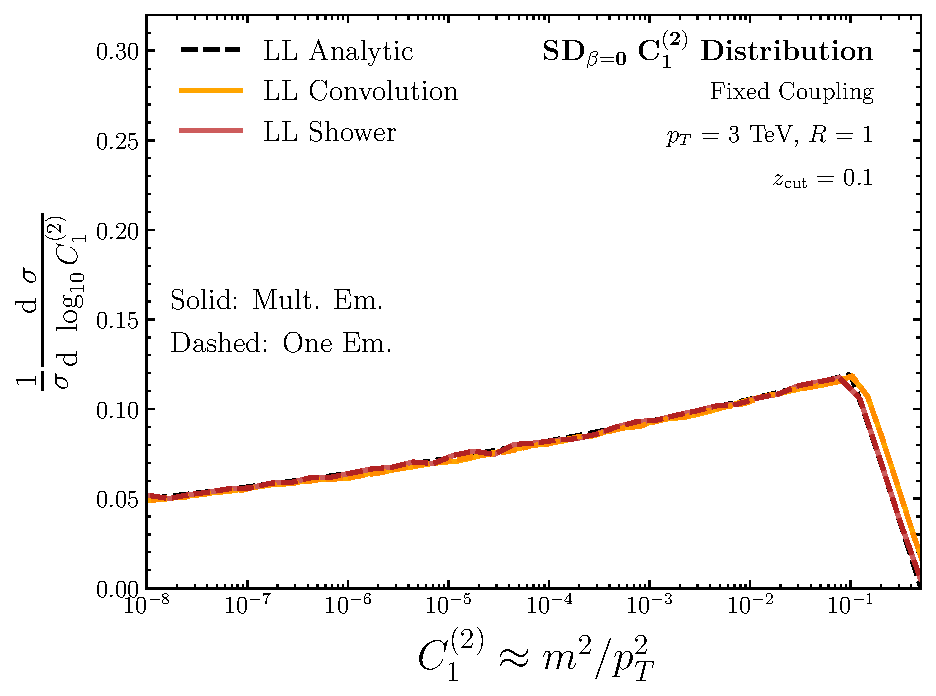
\includegraphics[width=.48\textwidth]{figures/piranha/resummed_plots/C12_SD0_LL}
\label{fig:LL_SD0}
}
%
% Soft Drop, MLL
\subfloat[]{
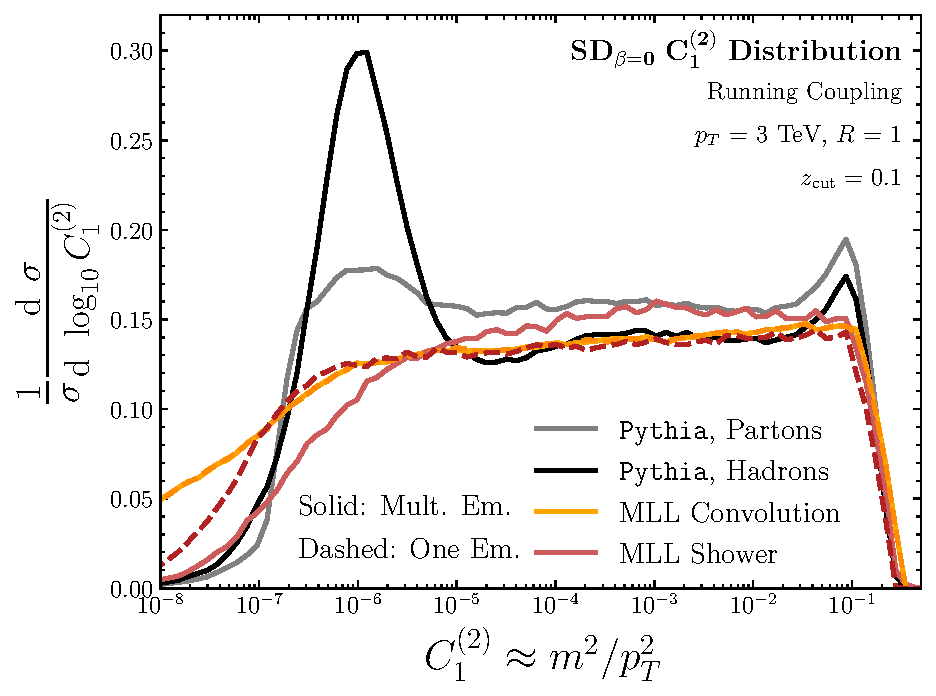
\includegraphics[width=.48\textwidth]{figures/piranha/resummed_plots/C12_SD0_MLL}
\label{fig:MLL_SD0}
}
\\
%
% \PRSF{1}, LL
\subfloat[]{
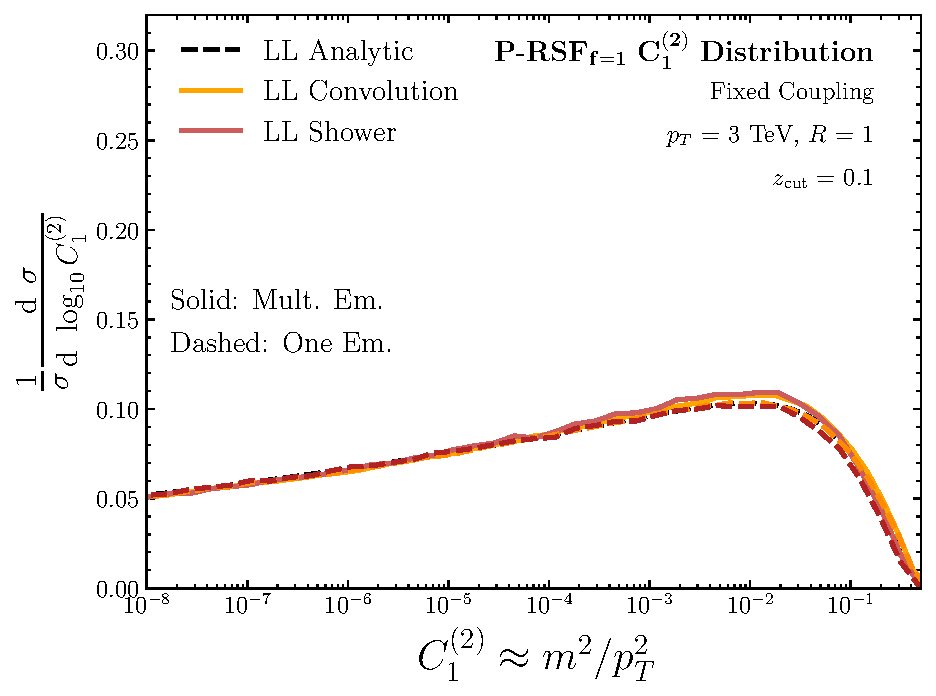
\includegraphics[width=.48\textwidth]{figures/piranha/resummed_plots/C12_PRSF1_LL}
\label{fig:LL_PRSF1}
}
%
% \PRSF{1}, MLL
\subfloat[]{
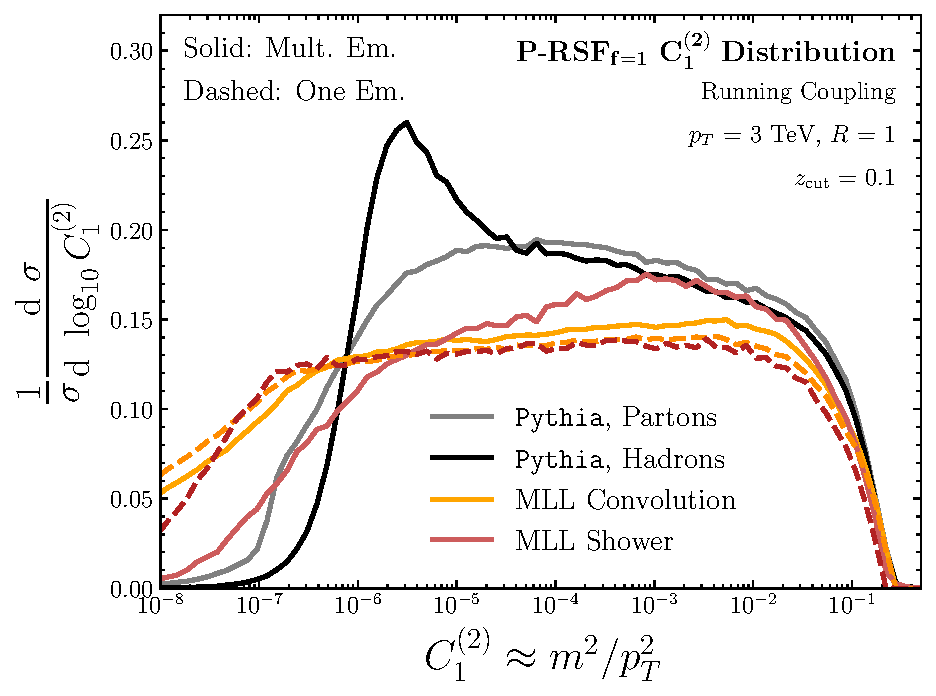
\includegraphics[width=.48\textwidth]{figures/piranha/resummed_plots/C12_PRSF1_MLL}
\label{fig:MLL_PRSF1}
}
\caption[Distributions of the observable \(C_1^{(2)}\approx m^2 / p_T^2\) for quark jets groomed with \SD{0} and \PRSF{1}.]{
Distributions of the observable \(C_1^{(2)}\approx m^2 / p_T^2\) of \Eq{ECFdefn_repeat} for quark jets groomed with \SD{0} (top row) and \PRSF{1} (bottom row), with and without multiple emissions, at (left column) LL accuracy and (right column) MLL accuracy.
%
For each plot, we display the results of the convolution method of \Eq{convolution} using numerical integration and \gls{pqcd} with \(10^6\) phase space samples as well as our own parton shower algorithm, discussed in \Prob{parton-shower} and its solution.
%
At LL, we compare these results to the analytic prediction of \Eq{ECF_LL};
%
at MLL, we compare them to parton-level and hadron-level results obtained with \texttt{Pythia 8.244} using the anti-\(k_t\) algorithm.
%
The figures demonstrate that \PRSF{1} is less sensitive to \gls{hadronization} corrections in the large observable regime, near \(C_1^{(2)} \approx 10^{-2}\), and that \PRSF{1} groomed substructure is more sensitive to the effects of multiple emissions than that of Soft Drop.
}
\label{fig:Calculations}
\end{figure}

As a result, performing resummed calculations of Soft Drop groomed substructure distributions that use only the critical emissions are more accurate than calculations for \PRSF{1} that only use the critical emission.
%
The relative accuracy of the LL, single-emission result for Soft Drop and \PRSF{1} is demonstrated in \Figs{LL_SD0}{LL_PRSF1}, which compares the fixed-order behavior of \(C_1^{(2)}\) distributions for jets groomed with Soft Drop or \PRSF{1}, respectively, using either the critical emission or all emissions in the jet.
%
Our parton shower procedure is inspired by \Reff{Larkoski:2013paa} and is exposed in more detail in Problem~\ref{prob:parton-shower}.
%
Including multiple emissions does not dramatically change the Soft Drop substructure distribution, but leads to non-negligible changes in \PRSF{1} substructure distributions.


%=====================================
% Modified Leading Logarithmic Calculation
%=====================================
We include effects from the running of the strong coupling constant and multiple emissions within the ungroomed jet to determine the behavior of the cumulative distribution of \(C_1^{(\varsigma)}\) at MLL accuracy.
%
While including these features in our calculation does not fully achieve next-to-leading-logarithmic (NLL) accuracy, the MLL calculation is an important piece of the full NLL result.
%
To consider the effects of several emissions on the distribution of the groomed ECFs, we convolve the probability distributions of several emissions that contribute to the total observable \(C_1^{(\varsigma)}\):

\begin{equation}
\begin{aligned}
    \rho^{\rm (MLL)}_\varsigma(C_{\rm tot})
    &=
    \int_{f\,\zcut}^{1/2} \dd \zcrit
    \int_0^R \dd \thetacrit
    ~
    \rho_{\rm crit}(\thetacrit)
    \rho_{\rm crit}(\zcrit | \zpre)
    \\
    &~~~
    \int \dd \zpre
    ~
    \rho_{\rm pre}(\zpre|\thetacrit)
    \int \dd c_{\rm sub}
    ~
    \rho_{\rm sub}(c_{\rm sub}|\zcrit,\thetacrit)
    \\
    &~~~~~~~~~~~~~~~
    \delta\left(
        C_{\rm tot}
        -
        C^{(\varsigma)}_{1,~\rm crit}
        (\thetacrit, \zcrit, \zpre)
        -
        c_{\rm sub}
    \right)
    \label{eq:convolution}
    .
\end{aligned}
\end{equation}

Each factor of \(\rho\) in \Eq{convolution} indicates a resummed probability distribution corresponding to a particular emission.
%
At the MLL level of accuracy, these resummed probability distributions are all calculated with a running coupling \(\alpha_s\).
%
We model non-perturbative effects by freezing the value of \(\alpha_s\) below the non-perturbative scale of \(\mu_{\rm freeze} = 1\) GeV, as in \Eq{frozencoupling}.
%
Variations in our choice of non-perturbative scale lead only to small changes to our results.


The expressions that describe multiple emissions within the groomed jet are:
\begin{itemize}
\item
\(\rho_{\rm crit}(\thetacrit) \rho(\zcrit | \zpre)\) represents the probability distribution for the emission angle \(\thetacrit\) and energy fraction \(\zcrit\) of the \textit{critical} emission, or the first emission to survive the \PRSF{1/2} procedure.
%
This distribution is conditioned on the presence of earlier emissions that modify the grooming procedure.

\item
\(\rho_{\rm pre}(\zpre | \thetacrit)\) encodes the probability that emissions that are wider than the critical emission, which we call \textit{pre-critical} emissions, have an energy fraction \(\zpre\).
%
%Here, \textit{dominant} means that this is the pre-critical emission with the largest value of the energy fraction \(\zpre\).
%
Any non-zero value of \(\zpre\) mitigates the grooming of the critical emission.

\item
\(\rho_{\rm sub}(c_{\rm sub} | \zcrit, \thetacrit)\) is the probability distribution for emissions narrower than the critical emission to contribute a value \(c_{\rm sub}\) to the overall observable \(C^{(\varsigma)}_1\).
%
We call these emissions \textit{subsequent} emissions, and they are unmodified by the grooming procedure.

\item
Finally, \(C^{(\varsigma)}_{1,~\rm crit}(\thetacrit,\zcrit,\zpre)\) is the contribution of the critical emission to \(C^{(\varsigma)}_{1,~\rm tot}\), in the presence of pre-critical emissions with energy fraction \(\zpre\).
\end{itemize}

\remark{}{
    We examine the effects of \glspl{precrit-emission} and \glspl{sub-emission} on \gls{rsf}-groomed \gls{gecf} distributions, including multiple emissions effects, using the multiple emissions formula \Eq{multiple-emissions} exposited by Problem~\ref{prob:multiple-emissions}.
    %
    In particular, if we have the radiator for an additive observable \(\mathcal O\), it is simple to evaluate corrections due to the presence of multiple emissions with Laplace transform methods \cite{Banfi:2004yd} to find that, at MLL accuracy,
    %
    \begin{align}
        \Sigma^{\rm (MLL)}_{\mathcal O}(x)
        &=
       \frac{
       e^{-R_{\mathcal O}(x)
       -
       \gamma_E R'_{\mathcal O}(x)}
       }
       {\Gamma
       \left(1 + R'_{\mathcal O}(x)\right)
       }
       \label{eq:mll_general_dist}
       ,
    \end{align}
    %
    where \(\gamma_E\) is the Euler-Mascheroni constant, and the prime denotes a derivative with respect to \(\log(1/x)\), lead us to the MLL expressions for the effects of multiple pre-critical and subsequent emissions on jet ECFs.
    %
    For example, the cumulative distribution for the contribution of the subsequent emissions to the observable \(C_1^{(\varsigma)}\) takes the form
    %
    \begin{align}
        \Sigma^{\rm(MLL)}_{C^{(\varsigma)}_{\rm sub}}
        (C  |  \thetacrit, \zcrit)
        &=
       \frac{
       e^{-R_{\rm sub}(C)
       -
       \gamma_E R'_{\rm sub}(C)}
       }
       {\Gamma
       \left(1 + R'_{\rm sub}(C)\right)
       }
       \approx
       e^{-R_{\rm sub}(C)}
       =
       \Sigma^{\rm(LL)}_{C^{(\varsigma)}_{\rm sub}}
       (C  |  \thetacrit)
       \label{eq:subsequentDist}
       ,
    \end{align}
    %
    where \(R_{\rm sub}(C)\) is shorthand for \(R_{C^{(\varsigma)}_{\rm sub}}(C | \thetacrit)\), defined as
    %
    \begin{align}
        R_{C^{(\varsigma)}_{\rm sub}}
        (C | \thetacrit)
        &=
        \begin{tikzpicture}[
        baseline={([yshift=-.8ex]current bounding box.center)},
        vertex/.style={anchor=base,
        circle,fill=black!25,minimum size=18pt,inner sep=2pt},
        scale=.3]
        \begin{axis}
        [xmin=0, xmax=5,
        ymin=0, ymax=5,
        axis line style = very thick,
        axis y line*=left,
        axis x line*=bottom,
        axis lines = middle,
        ticks=none]
            \addplot[name path=f,domain=0:5,
            style=very thick, blue]
            {4.5-1.5*x};
            \path[name path=axis]
            (axis cs:0,5) -- (axis cs:5,5);
            \addplot [
                thick,
                color=blue,
                fill=blue,
                fill opacity=0.3
            ]
            fill between[
                of=f and axis
            ];
            \node at (axis cs:  2.9,  3.8)
            {${\scriptstyle C_{\rm sub}^{(\varsigma)} > z\theta^\varsigma}$};
            \node at (axis cs:  3.4,  1.8)
            {${\scriptstyle \theta > \theta_{\rm crit}}$};
        \end{axis}
        \end{tikzpicture}
        =
        \int_{C/\thetacrit^{\varsigma}}^{1/2}
        \frac{\dd c}{c}
        \int_c^{1/2} \dd z\,
        \bar{p}_i(z)
        \frac{\alpha_s(\kappa)}{k \varsigma}
        .
    \end{align}
    Of course, the value of \zcrit{} will also have an impact on the subsequent emissions, but we may safely neglect these corrections, which contribute only by scaling \(C_{\rm sub}^{(\varsigma)}\) by factors of the form \(1 - \zcrit\).
    %
    The cumulative distribution for the energy fraction carried by pre-critical emissions is calculated similarly and takes the form
    %
    \begin{align}
        \Sigma^{\rm(MLL)}_{\zpre}
        (z | \thetacrit)
        &=
       \frac{
       e^{-R_{\rm pre}(z | \thetacrit)
       -
       \gamma_E R'_{\rm pre}(z | \thetacrit)}
       }
       {\Gamma
       \left(1 + R'_{\rm pre}(z | \thetacrit)\right)
       }
       \approx
       e^{-R_{\rm pre}(z | \thetacrit)}
       =
       \Sigma^{\rm(LL)}_{\zpre}
       (z  |  \thetacrit)
       \label{eq:preDist}
       ,
    \end{align}
    %
    where \(R_{\rm pre}(z | \thetacrit) = R_{\zpre}(z | \thetacrit)\) is given by
    %
    \begin{align}
        R_{\zpre}
        (z | \thetacrit)\
        &=
        \int_{\thetacrit}^{1}
        \frac{\dd\theta}{\theta}
        \int_{z}^{\zcut}\dd z'\,
        \bar{p}_i(z')
        \frac{\alpha_s(\kappa)}{\pi}
        .
    \end{align}
}

We evaluate the convolution of \Eq{convolution} -- including effects from the \gls{crit-emission}, \glspl{precrit-emission} and \glspl{sub-emission} -- through numerical integration, and compare the resulting distributions to the results from running coupling parton showers and \texttt{Pythia 8.244} in \Fig{Calculations}.
%
In particular, \Figs{MLL_SD0}{MLL_PRSF1} compare our numerical MLL results to hadron-level results for anti-\(k_t\) jets in \texttt{Pythia 8.244} and demonstrate that this trend of comparatively large multiple-emissions effects in \PRSF{1} continues at MLL.

First, let us note the difference between our MLL results obtained with Monte Carlo integration and via parton showers (as in Problem~\ref{prob:parton-shower}).
%
Our Monte Carlo results use a frozen coupling below a non-perturbative scale \(\mu_{\rm freeze} = 1\) GeV (see, for example, \Eq{frozencoupling} of \App{soft-distortions}).
%
Our parton shower results both freeze the coupling at \(\mu_{\rm freeze} = 1\) GeV and stop the shower below a non-perturbative cutoff \(\mu_{\rm cutoff} = 1\) MeV, tuned by hand to match results from \texttt{Pythia 8.244}.
%
The shower cutoff effectively sets \(\alpha_s\) to zero below the scale set by \(\mu_{\rm cutoff}\).
%
Therefore, the plots in \Figs{MLL_SD0}{MLL_PRSF1} effectively show the results obtained with three different models of non-perturbative effects, with \texttt{Pythia 8.244} the most accurate.
%
Our MLL parton shower results in \Figs{MLL_SD0}{MLL_PRSF1} are still normalized, but the normalization is not immediately evident due to the presence of zero bins that are not shown in the logarithmically-scaled figures.
%
In passing from our rough parton shower model to the more accurate \gls{hadronization} model of \texttt{Pythia}, we expect that it is these zero bins that contribute to the additional hadron-level peak shown in the \texttt{Pythia} data.

We also point out that in \Fig{MLL_SD0}, the parton-level \texttt{Pythia 8.244} distribution for \(C_1^{(2)}\) also has an additional peak near the discontinuity in the parton-level LL result, in the regime of relatively large \(C_1^{(2)} \approx 10^{-1}\).
%
There is a comparable additional peak in the hadron-level \texttt{Pythia} distribution for \(C_1^{(2)}\) at this relatively large value for the observable.

We also note that, while our numerical results for \PRSF{1} in the MLL figures agree roughly with \texttt{Pythia 8.244} in the regime of large \(C_1^{(2)}\), the hadron-level \texttt{Pythia} distributions have an additional peak near \(C_1^{(2)} \approx 3\times 10^{-6}\) due to \gls{hadronization} corrections to the observable at that scale.
%
There is a similar additional peak in the hadron-level \texttt{Pythia} distribution for mMDT (\SD{0}) groomed \(C_1^{(2)}\).


% \begin{example}
%     \label{ex:conditionalprecrit}
%     Let's compute a conditional probability distribution relevant for the physics of Example \ref{ex:z_precrit}. In particular, let's compute the conditional probability distribution \(\rho(z_{\rm pre} | \theta_{\rm crit})\) to find a pre-critical emission with a maximum possible angle. We should first remember the solution to Example \ref{ex:z_precrit}, which gives us an overall probability distribution
%     \begin{equation}
%     \begin{aligned}
%         \rho(z_{\rm pre}, \theta_{\rm crit})
%         &=
%         \left(\frac{2 C_R \alpha_{\rm S}}{\pi}\right)^2
%         \frac{1}{\theta}
%         \log(\theta_{\rm crit})
%         [p(z_{\rm pre})]_+
%         \int_{z > z_{\rm pre}} z~\dd\log(z) [p(z)]_+
%         \\
%         &\ \ \ \ \ \ \ \ \ \ \
%         \times
%         \exp\left[
%         ~-~
%         \begin{tikzpicture}
%         [baseline={([yshift=-.8ex]current bounding box.center)},
%         vertex/.style={anchor=base,
%         circle,fill=black!25,minimum size=18pt,inner sep=2pt},
%         scale=.3]
%         \begin{axis}
%         [xmin=0, xmax=5,
%         ymin=0, ymax=5,
%         axis line style = very thick,
%         axis y line*=left,
%         axis x line*=bottom,
%         axis lines = middle,
%         ticks=none]
%             \addplot[name path=f,domain=0:2.3,
%             style=very thick,blue]
%             {2.5};
%             \addplot[very thick, samples=50, smooth,domain=0:6,blue, name path=three] coordinates {(2.3,-1)(2.3,2.5)};
%             \path[name path=axis]
%             (axis cs:0,0) -- (axis cs:2.3,0);

%             \addplot[name path=pre,domain=0:2.3,
%                     style=very thick,magenta]
%                     {2.6};
%             \addplot[name path=pre2,domain=0:2.3,
%                     style=very thick,magenta]
%                     {4.};
%             \addplot[very thick, samples=50, smooth,domain=0:6,magenta, name path=three] coordinates {(2.3,2.525)(2.3,4)};
%             \path[name path=axispre]
%             (axis cs:0,4) -- (axis cs:2.3,4);
%             \addplot [
%                 thick,
%                 color=blue,
%                 fill=blue,
%                 fill opacity=0.3
%             ]
%             fill between[
%                 of=f and axis
%             ];
%             \addplot [
%                 thick,
%                 color=magenta,
%                 fill=magenta,
%                 fill opacity=0.3
%             ]
%             fill between[
%                 of=pre and axispre
%             ];
%         \end{axis}
%         \end{tikzpicture}
%         ~~
%         \right]
%         .
%     \end{aligned}
%     \end{equation}


%     On the other hand, the probability distribution for \(\theta_{\rm crit}\) alone can be quickly read off from the solution to Example \ref{ex:theta_crit}:
%     \begin{equation}
%     \begin{aligned}
%         \rho(\theta_{\rm crit})
%         =
%         \frac{2 C_R \alpha_{\rm S}}{\pi}
%         ~
%         \frac{1}{\theta_{\rm crit}}
%         \int_{z > z_{\rm cut}} [p(z)]_+
%         ~~
%         \exp\left[
%         ~-~
%         \begin{tikzpicture}[
%         baseline={([yshift=-.8ex]current bounding box.center)},
%         vertex/.style={anchor=base,
%         circle,fill=black!25,minimum size=18pt,inner sep=2pt},
%         scale=.3]
%         \begin{axis}
%         [xmin=0, xmax=5,
%         ymin=0, ymax=5,
%         axis line style = very thick,
%         axis y line*=left,
%         axis x line*=bottom,
%         axis lines = middle,
%         ticks=none]
%         	\addplot[name path=f,domain=0:2.3,
%             style=very thick,blue]
%             {2.5};
%             \addplot[very thick, samples=50, smooth,domain=0:6,blue, name path=three] coordinates {(2.3,-1)(2.3,2.5)};
%             \path[name path=axis]
%             (axis cs:0,0) -- (axis cs:2.3,0);
%             \addplot [
%                 thick,
%                 color=blue,
%                 fill=blue,
%                 fill opacity=0.3
%             ]
%             fill between[
%                 of=f and axis
%             ];
%         \end{axis}
%         \end{tikzpicture}
%         ~~
%         \right]
%         .
%     \end{aligned}
%     \end{equation}

%     Finally, we can easily write the corresponding conditional probability
%     \begin{equation}
%     \begin{aligned}
%         \rho(z_{\rm pre}|\theta_{\rm crit})
%         &=
%         \frac{\rho(z_{\rm pre},\theta_{\rm crit})}{\rho(\theta_{\rm crit})}
%         \\
%         &=
%         \frac{2 C_R \alpha_{\rm S}}{\pi}
%         ~
%         \log(\theta_{\rm crit})
%         ~
%         [p(z_{\rm pre})]_+
%         ~
%         \frac{\int_{z > z_{\rm pre}} z~\dd\log(z) p(z)}
%         {\int_{z > z_{\rm cut}} z~\dd\log(z) p(z)}
%         ~~
%         \exp\left[
%         ~-~
%         \begin{tikzpicture}
%         [baseline={([yshift=-.8ex]current bounding box.center)},
%         vertex/.style={anchor=base,
%         circle,fill=black!25,minimum size=18pt,inner sep=2pt},
%         scale=.3]
%         \begin{axis}
%         [xmin=0, xmax=5,
%         ymin=0, ymax=5,
%         axis line style = very thick,
%         axis y line*=left,
%         axis x line*=bottom,
%         axis lines = middle,
%         ticks=none]
%             \addplot[name path=pre,domain=0:2.3,
%                     style=very thick,magenta]
%                     {2.6};
%             \addplot[name path=pre2,domain=0:2.3,
%                     style=very thick,magenta]
%                     {4.};
%             \addplot[very thick, samples=50, smooth,domain=0:6,magenta, name path=three] coordinates {(2.3,2.525)(2.3,4)};
%             \path[name path=axispre]
%             (axis cs:0,4) -- (axis cs:2.3,4);
%             \addplot [
%                 thick,
%                 color=magenta,
%                 fill=magenta,
%                 fill opacity=0.3
%             ]
%             fill between[
%                 of=pre and axispre
%             ];
%         \end{axis}
%         \end{tikzpicture}
%         ~~
%         \right]
%         \\
%         &\approx
%         \frac{2 C_R \alpha_{\rm S}}{\pi}
%         ~
%         \log(\theta_{\rm crit})
%         ~
%         \left[\frac{1}{z_{\rm pre}}\right]_+
%         \frac{\log(z_{\rm cut} / z_{\rm pre})}{\log(z_{\rm cut})}
%         ~
%         z_{\rm pre}^{~~\frac{2 C_R \alpha_{\rm S}}{\pi}\log(\theta_{\rm crit})}.
%     \end{aligned}
%     \end{equation}
% \end{example}

We need only use the singular pieces of the splitting functions to achieve LL accuracy, but, by definition, we must include the non-singular pieces of the splitting functions to achieve MLL accuracy.
%
While the MLL analysis modifies the LL analysis by including additional, higher-order behavior, it is not quite sufficient to produce results at next-to-leading logarithmic (NLL) accuracy;
%
a full NLL result requires a more intricate treatment including the effects of logarithms due to the constraint that radiation within the jet must lie within the jet radius.
%
These logarithms emerge because jet observables depend on only subsets of the full phase (global) space of the outgoing radiation, and are known as non-global logarithms \cite{Dasgupta:2001sh,Dasgupta:2002dc,Dasgupta:2002bw,Banfi:2002hw,Appleby:2002ke,Weigert:2003mm,Rubin:2010fc,Banfi:2010pa,Kelley:2011tj,Hornig:2011iu,Kelley:2011aa,Hatta:2013iba,Schwartz:2014wha,Khelifa-Kerfa:2015mma,Larkoski:2015zka,Larkoski:2016zzc,Banfi:2021owj}.
%
Regardless, the MLL results presented in the paper provide a sense of the physics contained within NLL results.



%==============================================
\section{Discontinuities in Grooming}
%==============================================
\label{sec:discontinuity}

In this section, we examine the formal structure of discontinuities in grooming in greater detail, and explore the improved continuity of \PIRANHA{} conceptually through several toy examples.
%
We compare the leading order (LO) soft continuity properties of Soft Drop and Recursive Subtraction both conceptually (\Sec{sd_discont}) and through a perturbative calculation (\Sec{sd_discont_lo}).
%
In \Secs{rsf_discont}{ang_discont}, we explore potential challenges to continuity that can arise in more intricate scenarios.
%
In particular, a key result of this section is that it is \textit{impossible} to design a fully continuous, tree-based \gls{declustering} algorithm.
%
Specifically, we discuss suppressed soft discontinuities that emerge in Unbalanced Recursive Subtraction (\Sec{rsf_discont}) and angular discontinuities induced by angular-ordered jet clustering that emerge beyond \glslink{accuracy}{NLO} in tree-based grooming algorithms (\Sec{ang_discont}).
%
We do not delve into the mathematical intricacies or perturbation theory of these examples, and they may be skipped on an initial reading.
%
The qualitative continuity properties explored in this section are also summarized at the beginning of the chapter, and contrasted against the discontinuities of traditional groomers, in \Tab{groomerlist}.
%
We explore the improved continuity of \PIRANHA{} groomers in a more practical context in \Sec{grooming-pheno}, where we study the responses of \PIRANHA{} grooming to several sources of \glspl{soft-distortion} and \gls{additive-contamination}.


The modified Mass Drop Tagger (mMDT, or \SD{0}) \cite{Dasgupta:2013ihk,Larkoski:2014wba}, for example, requires that certain sub-jets within a jet carry a sufficient energy fraction, \(z > z_{\rm cut}\), to survive the grooming procedure.
%
If a sub-jet has an energy fraction near \(\zcut\), low-energy pollution may push its energy to the other side of the cutoff, leading to soft discontinuous behavior and associated theoretical and experimental complications.
%
\Fig{grooming-cartoon} demonstrates this soft discontinuous behavior, and the corresponding soft continuity of \PRSF{1/2}, by comparing their action on two sets of similar events:
%
two toy jet events \(\mathcal{E}^\pm\) consisting of two particles each, and a QCD jet produced in \texttt{Pythia 8.244} along with the same QCD event with a small amount of gaussian noise applied to the \(p_T\), rapidity, and azimuthal angle of each particle.
%
We revisit the events \(\mathcal{E}^\pm\) as tools to characterize soft discontinuity more precisely in \Sec{sd_discont}.
%
The mMDT grooming procedure maps \(\mathcal{E}^+\) and \(\mathcal{E}^-\) to very distinct events, and similarly maps the noiseless and noisy QCD jets to very distinct groomed jets.
%
We chose an unusually high value of \(\zcut = 0.25\) when grooming the QCD events to make the discontinuity of mMDT more apparent.
%
\footnotetext{
Soft Drop with \(\beta_{\rm SD} \leq 0\) is not collinear safe in grooming mode, used in this thesis, where jets consisting of a single particle are retained as groomed jets.
%
Grooming mode is a natural choice in the context of \gls{pu-mitigation} (see \Sec{sd_discont}).
%
Note that Soft Drop with \(\beta_{\rm SD} \leq 0\) is collinear safe in tagging mode, where jets consisting of a single particle are groomed away completely.
}

%=====================================
% Simple Demonstration of Continuity:
%=====================================
\subsection{An Invitation to Soft Discontinuities: Soft Drop Versus P-RS}
\label{sec:sd_discont}

%-----------------------------------
% Cartoon of comparison:
%-----------------------------------
\begin{figure}[]
\centering
\scalebox{0.95}{
    \begin{tikzpicture}[baseline=-3.5ex]
% Event Labels
  \node at (-1.7,  .6)()
        {\huge \(\mathcal{E}^+\)};
  \node at (-1.7,  -1.25)()
        {\huge\(\mathcal{E}^-\)};

% Header wrapper
\draw [fill=black, opacity=0.05]
       (-0.7,2.4) -- (13.6,2.4) -- (13.6,1.65) -- (-0.7,1.65) -- cycle;

%%%%%%%%%%%%%%
% Ungroomed
%%%%%%%%%%%%%%
  \node at (1.5,  2)() {\textbf{Ungroomed}};

% E+
  % points
  \coordinate (A)  at (1.4, 1.4);
  \coordinate (O)  at (0, 0);
  \coordinate (B)  at (3, 0);
  % legs
  \draw[-Stealth,line width=.55mm] (O) -> (A);
  \draw[-Stealth,line width=.7mm] (O) -> (B);

% E-
  % points
  \coordinate (A)  at (.8, -1.2);
  \coordinate (O)  at (0, -2);
  \coordinate (B)  at (3, -2);
  % legs
  \draw[-Stealth,line width=.55mm] (O) -> (A);
  \draw[-Stealth,line width=.7mm] (O) -> (B);

% lines

% zcut lines
\coordinate (I)  at (0.7, 1.0);
\coordinate (F)  at (3.15, 1.0);
\draw[dash pattern=on 2pt off 3pt, line width=.4mm, color=aurometalsaurus] (I) -> (F);
\node at (3.5,  1.0)()
        {\(\zcut\)};

\coordinate (I)  at (0.7, -1.0);
\coordinate (F)  at (3.15, -1.0);
\draw[dash pattern=on 2pt off 3pt, line width=.4mm, color=aurometalsaurus] (I) -> (F);
\node at (3.5,  -1.0)()
        {\(\zcut\)};

% Descriptors
\node [rotate=45] at (0.0,  0.5)()
        {\(z^+ > \zcut\)};
\node [rotate=45] at (0.0,  -1.5)()
        {\(z^- < \zcut\)};


%%%%%%%%%%%%%%
% Soft Drop Grooming
%%%%%%%%%%%%%%
\node at (6.5,  2)() {\textcolor{dodgerblue!75!black}{\textbf{Soft Drop}, \(\beta_{\rm SD} = 0\)}};

% E+
  % points
  \coordinate (A)  at (6.4, 1.4);
  \coordinate (O)  at (5.0, 0);
  \coordinate (B)  at (8.0, 0);
  % legs
  \draw[-Stealth,line width=.55mm, color=royalblue] (O) -> (A);
  \draw[-Stealth,line width=.7mm, color=royalblue] (O) -> (B);

% E-
  % points
  \coordinate (Ap)  at (5.8, -1.2);
  \coordinate (O)  at (5.0, -2);
  \coordinate (B)  at (8.0, -2);
  % legs
  \draw[-Stealth, line width=.55mm, color=black!25!white] (O) -> (Ap);
  \draw[-Stealth,line width=.7mm, color=royalblue] (O) -> (B);

% lines
% zcut lines
\coordinate (I)  at (5.7, 1.0);
\coordinate (F)  at (8.15, 1.0);
\draw[dash pattern=on 2pt off 3pt, line width=.4mm, color=aurometalsaurus] (I) -> (F);

\coordinate (I)  at (5.7, -1.0);
\coordinate (F)  at (8.15, -1.0);
\draw[dash pattern=on 2pt off 3pt, line width=.4mm, color=aurometalsaurus] (I) -> (F);

%%%%%%%%%%%%%%
% PIRANHA Grooming \PRSF{1/2}
%%%%%%%%%%%%%%
  \node at (10.9,  2)() {\textcolor{ochre!75!black}{\textbf{P-RSF} (arb.\,\(f_{\rm soft}\))}};

% E+
  % points
  \coordinate (A)  at (10.4, 0.9);
  \coordinate (Ap)  at (10.9, 1.4);
  \coordinate (O)  at (9.5, 0);
  \coordinate (B)  at (11.7, 0);
  \coordinate (Bp)  at (12.5, 0);
  % legs
  \draw[-Stealth,line width=.55mm, color=black!25!white] (O) -> (Ap);
  \draw[-Stealth,line width=.55mm, color=darkgoldenrod] (O) -> (A);
  \draw[-Stealth,line width=.7mm, color=black!25!white] (O) -> (Bp);
  \draw[-Stealth,line width=.7mm, color=darkgoldenrod] (O) -> (B);

% E-
  % points
  \coordinate (A)  at (9.9, -1.6);
  \coordinate (Ap)  at (10.3, -1.2);
  \coordinate (O)  at (9.5, -2);
  \coordinate (B)  at (11.7, -2);
  \coordinate (Bp)  at (12.5, -2);
  % legs
  \draw[-Stealth,line width=.55mm, color=black!25!white] (O) -> (Ap);
  \draw[-Stealth,line width=.55mm, color=darkgoldenrod] (O) -> (A);
  \draw[-Stealth,line width=.7mm, color=black!25!white] (O) -> (Bp);
  \draw[-Stealth,line width=.7mm, color=darkgoldenrod] (O) -> (B);

% lines
% zcut lines
\coordinate (I)  at (10.2, 1.0);
\coordinate (F)  at (12.65, 1.0);
\draw[dash pattern=on 2pt off 3pt, line width=.4mm, color=aurometalsaurus] (I) -> (F);

\coordinate (I)  at (10.2, -1.0);
\coordinate (F)  at (12.65, -1.0);
\draw[dash pattern=on 2pt off 3pt, line width=.4mm, color=aurometalsaurus] (I) -> (F);

%%%%%%%%%%%%%%
% QCD
%%%%%%%%%%%%%%
% Double line
\coordinate (I)  at (-2.5, -2.8);
\coordinate (F)  at (13.3, -2.8);
\draw[line width=.3mm] (I) -> (F);

\coordinate (I)  at (-2.5, -2.9);
\coordinate (F)  at (13.3, -2.9);
\draw[line width=.3mm] (I) -> (F);

% Labels
  \node at (-1.7,  -4.6)()
        {\textbf{\LARGE QCD}};
  \node at (-2.55, -5.8)(){\Large (};
  \node at (-1.7,  -5.6)()
        {\texttt{Pythia}};
  \node at (-1.7,  -6.0)()
        {\texttt{8.244}};
 \node at (-0.85, -5.8)(){\Large )};
  \node at (-1.7,  -8.4)()
         {\textbf{\LARGE QCD}};
 \node at (-1.7,  -9.0)()
         {\textbf{\Large +}};
 \node at (-1.7,  -9.6)()
        {\textbf{\LARGE Noise}};

% Event visualization
% Ungroomed
  \node at (1.8,  -5.0)() {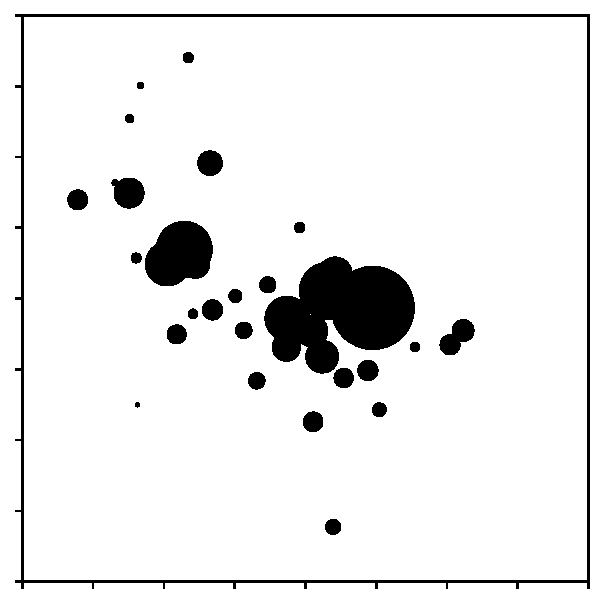
\includegraphics[width=.25\textwidth]{figures/piranha/event_visualizations/vis_raw_1}};
  \node at (1.8,  -9.0)() {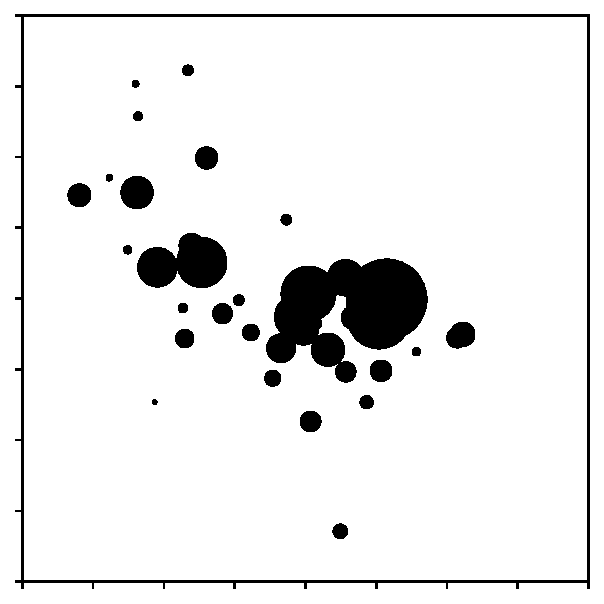
\includegraphics[width=.25\textwidth]{figures/piranha/event_visualizations/vis_raw_2}};
% mMDT
  \node at (6.5,  -5.0)() {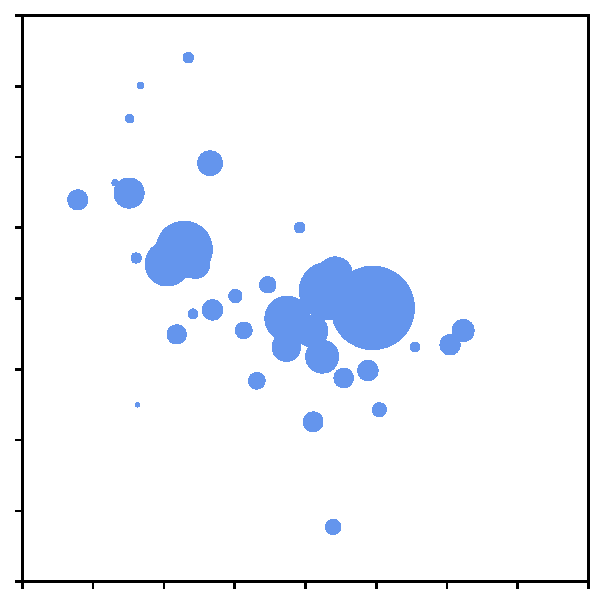
\includegraphics[width=.25\textwidth]{figures/piranha/event_visualizations/vis_mmdt_1}};
  \node at (6.5,  -9.0)() {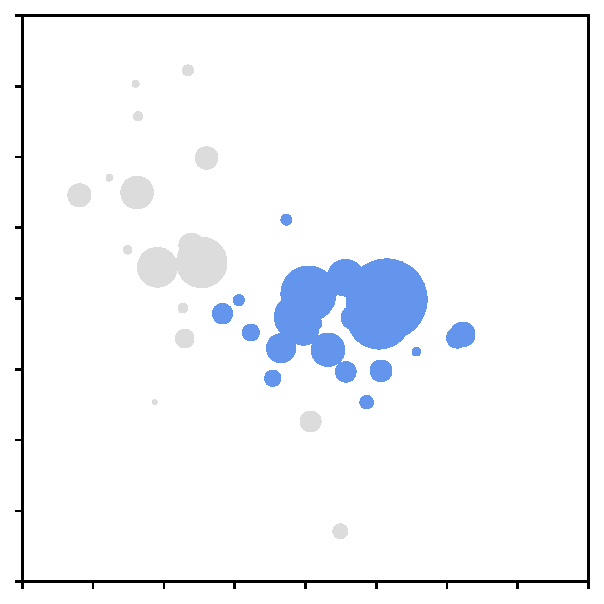
\includegraphics[width=.25\textwidth]{figures/piranha/event_visualizations/vis_mmdt_2}};
% P-RSF_1/2
  \node at (11.3,  -5.0)() {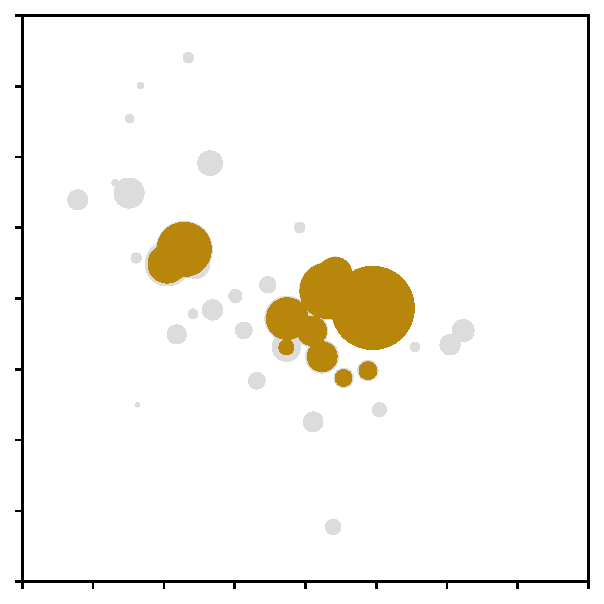
\includegraphics[width=.25\textwidth]{figures/piranha/event_visualizations/vis_rsf_half_1}};
  \node at (11.3,  -9.0)() {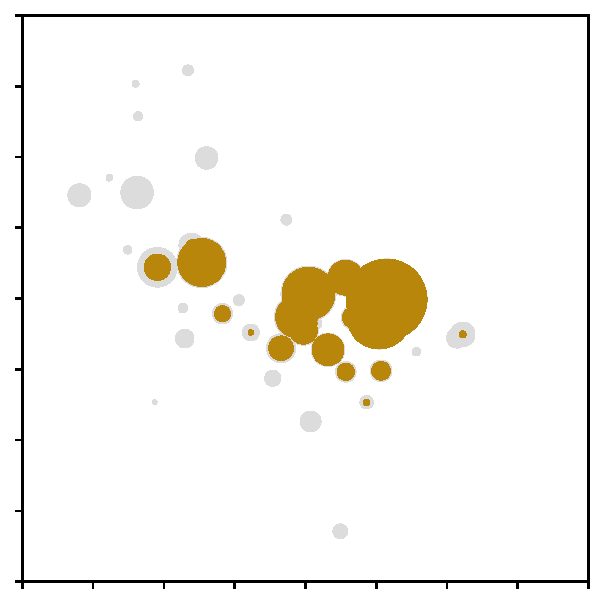
\includegraphics[width=.25\textwidth]{figures/piranha/event_visualizations/vis_rsf_half_2}};

% Axis info
 \node at (-0.4,  -5.0)() {\Large \(\phi\)};
 \node at (-0.4,  -9.0)() {\Large \(\phi\)};
 \node at (1.8,  -11.2)() {\Large \(y\)};
 \node at (6.5,  -11.2)() {\Large \(y\)};
 \node at (11.3,  -11.2)() {\Large \(y\)};

 % phi labels
 \node at (-0.25,  -10.77)() {\footnotesize -1};
 \node at (-0.25,  -7.3)() {\footnotesize 1};
 \node at (-0.25,  -6.77)() {\footnotesize -1};
 \node at (-0.25,  -3.3)() {\footnotesize 1};
 % y labels
 \node at (-0.05,  -11.1)() {\footnotesize -1};
 \node at (3.65,  -11.1)() {\footnotesize 1};
 \node at (4.65,  -11.1)() {\footnotesize -1};
 \node at (8.35,  -11.1)() {\footnotesize 1};
 \node at (9.45,  -11.1)() {\footnotesize -1};
 \node at (13.15,  -11.1)() {\footnotesize 1};

 %\node at (1.8,  -5.0)() {-1.0};
\end{tikzpicture}

}
\caption[A cartoon comparing the discontinuous action of hard-cutoff grooming to the continuous action of \PIRANHA{}.]{
A cartoon comparing the discontinuous action of hard-cutoff grooming to the continuous action of \PIRANHA{} on the nearly identical two-particle events with energy \(Q\), \(\mathcal{E}^+\) and \(\mathcal{E}^-\).
%
We use Soft Drop (with \(\beta_{\rm SD} = 0\)) and P-RSF (with arbitrary \(f_{\rm soft}\)) with a grooming parameter \zcut{} as representative examples of the hard-cutoff and \PIRANHA{} paradigms, respectively.
%========
% Ungroomed
%========
The events \(\mathcal E^\pm\) differ only by the energy fraction of the softer particle,
%
\(
z^\pm = \zcut \pm \delta/2
\),
%
and are separated by an infinitesimal EMD,
%
EMD\(
(\mathcal{E}^+, \mathcal{E}^-)
\sim \delta \ll \zcut
\).
%========
% SD
%========
Despite their similarity, Soft Drop maps the events to distinct groomed results separated by a large EMD:
%
%it removes no energy from \(\mathcal E^+\) (\(\Delta E^+_{\rm SD} = 0\)) and completely removes the softer particle from \(\mathcal E^-\) (\(\Delta E^-_{\rm SD} \sim Q z^-\)).
%
%and the Soft Drop groomed results are separated by a large EMD of
%
EMD\(
(\mathcal{E}_{\rm SD}^+, \mathcal{E}_{\rm SD}^-)
\sim \zcut \gg \delta
\).
%========
% P-RSF
%========
P-RSF instead
% subtracts a similar energy from both events (\(\Delta E^\pm_{\rm P\mhyphen RSF} \sim Q \zcut\)) and
maps the events continuously to infinitesimally similar groomed events:
%
EMD\(
(\mathcal{E}_{\rm P\mhyphen RSF}^+,
\mathcal{E}_{\rm P\mhyphen RSF}^-)
\sim \delta
\).
%
\(\Delta E^\pm_G\) indicates the amount of energy removed from the event \(\mathcal E^\pm\) by the groomer \(G\).
}
\label{fig:grooming-cartoon}
\end{figure}


%-----------------------------------
% Text comparison:
%-----------------------------------
Traditional groomers are discontinuous in the regions of parameter space near a hard cutoff.
%
For example, Soft Drop is discontinuous in the region of parameter space where
\(
    z_{\rm soft} = \zcut \theta^{\beta_{\rm SD}} / R_0^{\beta_{\rm SD}}
\)
due to the Soft Drop criterion of \Eq{softdropcriterion}.
%
In this subsection, we discuss the discontinuity of hard-cutoff grooming and the relative continuity of \PIRANHA{}.

The following discussion centers around the illustrative example shown in \Fig{grooming-cartoon}, which shows the simplest instance of discontinuous behavior near a hard cutoff as well as the resolution offered by \PIRANHA{}.
%
In this example, we consider two nearly identical events, \(\mathcal{E}^+\) and \(\mathcal{E}^-\), that each contain two particles.
%
The softer constituent of \(\mathcal E^+\) has an energy fraction \(z^+ =  \zcut + \delta\) slightly above the grooming parameter \zcut, while the softer constituent of \(\mathcal E^-\) has an energy fraction \(z^- =\zcut - \delta\) slightly below \zcut.
%
The energy flows of the two events are nearly indistinguishable, in the sense that \(
{\rm EMD}(\mathcal{E}^+, \mathcal{E}^-)\sim\delta
\),
and we choose \(\delta\) for consistency with Definition~\ref{def:eventcontinuity}.
%
We use Soft Drop with \(\beta_{\rm SD} = 0\), or mMDT, as a representative example of hard-cutoff grooming, and P-RSF with arbitrary \(f_{\rm soft}\) as a representative example of the \PIRANHA{} paradigm;
%
for each, we use the parameter \(\zcut\).

Soft Drop treats \(\mathcal E^+\) and \(\mathcal E^-\) very differently:
%
it does not modify \(\mathcal E^+\), but completely removes the softer particle of \(\mathcal E^-\).
%
The energy flow of \(\mathcal E^+\) is unchanged, while that of \(\mathcal E^-\) is changed dramatically, and the EMD between the groomed jets is relatively large:
EMD\(
(\mathcal{E}^+_{\rm SD},
\mathcal{E}^-_{\rm SD})
\sim \zcut
\gg \delta\).
%
Direct application of Definition~\ref{def:eventcontinuity} to our example shows that Soft Drop is discontinuous.\footnote{
We note that Soft Drop with \(\beta \neq 0\) is also soft discontinuous.
%
Indeed, the above arguments still hold for the case \(\beta \neq 0\), verbatim, when the angle between the particles of \(\mathcal E^\pm\) is fixed to \(\theta = R_0\).
%
As expressed in \Eq{softdropcriterion}, the Soft Drop criterion at this fixed angle is still \(z_{\rm soft} > \zcut\).
%
However, since Soft Drop with \(\beta \neq 0\) drops the softer particle if it does not satisfy \(z / \theta^{\beta} > \zcut/ R_0^\beta\), we may also say that Soft Drop with \(\beta \neq 0\) is ``\(z / \theta^{\beta}\)-discontinuous'', where \(z\)-discontinuity indicates the soft discontinuity for the case of \(\beta = 0\) that we discuss above.
}
%
Since the events \(\mathcal E^+\) and \(\mathcal E^-\) differ by small changes to the energy of jet constituents, we see that Soft Drop is soft discontinuous in the region of parameter space near the cutoff \zcut.

The procedure of P-RSF is quite different.
%
When grooming both events, \PRSF{1/2} grooms the energy of both emissions by the same amount, leading to no large discrepancy in the two groomed results.
%
Indeed, after the \PRSF{1/2} grooming procedure, these two events are still separated by an infinitesimal EMD:
EMD\((\mathcal{E}^+_{\rm RSF},
\mathcal{E}^-_{\rm RSF})\sim\delta\).
%
This simple example demonstrates how hard-cutoff grooming methods may discontinuously map two nearly identical events into vastly different groomed results, and showcases the soft continuous resolution of the \PRSF{1/2} grooming procedure and other \PIRANHA{} groomers.


%=====================================
% Discontinuity in SD in LO calculation
%=====================================

\subsection{Soft Discontinuities in Perturbation Theory}
\label{sec:sd_discont_lo}

Next, we examine the manifestations of the soft discontinuous behavior of hard-cutoff grooming more quantitatively by comparing the \gls{gecf} distributions of jets groomed with \gls{soft-drop} and \gls{rsf} at NLO.
%
The resummed analysis of \Sec{pira-resummed} does not change the qualitative conclusions of our discussion below.
%
However, it highlights subtleties in systematically improving our resummed substructure calculations due to the global, subtractive nature of \PIRANHA{} grooming.
%
Therefore, while our resummation does not change the qualitative conclusions of the following discussion, it indicates that the computation of resummed \PIRANHA{} observables at higher accuracy may require new calculational tools.


The probability distribution of \(C_1^{(\varsigma)}\) for Soft Drop was studied in \Reff{Larkoski:2014wba} (see Exercise~\ref{ex:soft-drop-gecf}), which found, for \(\beta_{\rm SD} > 0\), the \glslink{accuracy}{NLO} result
\begin{align}
    \label{eq:sd_lo}
    \rho_{i,\,\,\text{SD}}(C_1^{(\varsigma)})
    \approx
    \frac{2\alpha_s C_{R_i}}{\pi \varsigma} \frac{1}{C_1^{(\varsigma)}}
    \times
    \begin{cases}
        -\log C_1^{(\varsigma)} + B_i,
        &
        C_1^{(\varsigma)} > \zcut;
        \\
        -
        \frac{\beta_{\rm SD}}{\varsigma+\beta_{\rm SD}} \log C_1^{(\varsigma)}
        -
        \frac{\varsigma}{\varsigma+\beta_{\rm SD}}\log \zcut
        +
        B_i,
        &
        C_1^{(\varsigma)} < \zcut,
    \end{cases}
\end{align}
away from \(C_1^{(\varsigma)} = 0\), up to \(\mathcal{O}(\alpha_s^2)\) and terms that are power suppressed in \(C_1^{(\varsigma)}\), \zcut, or both.
%
\(B_i\) is a factor due to hard-collinear pieces of the splitting function that are not singular as \(z\) approaches 0:
%
$B_q = -3/4$ for quarks and $B_g = -11/12+n_f/(6 C_A)$ for gluons, where $n_f$ is the number of active quark flavors.
%
The case \(\beta_{\rm SD} < 0\) leads to an identical result up to another constraint on \(C_1^{(\varsigma)}\), which simply multiplies the expression above by \(\Theta(C_1^{(\varsigma)} > \zcut^{\varsigma/ |\beta_{\rm SD}|})\).

The piece-wise behavior of \Eq{sd_lo} and the associated kink in the Soft Drop \(C_1^{(\varsigma)}\) distribution are due to the discontinuous behavior of Soft Drop.
%
As noted by \Reff{Larkoski:2014wba}, when \(\beta_{\rm SD} \geq 0\) any two-parton configurations with \(C_1^{(\varsigma)} = z \, (\theta/R_0)^\varsigma \, > \, \zcut\) must have \(z \, (\theta/R_0)^{\beta_{\rm SD}} \, > \, \zcut\), and are therefore not affected by Soft Drop.
%
On the other hand, configurations with \(C_1^{(\varsigma)} < \zcut\) may be Soft Dropped, leading to the piece-wise change in groomed substructure in this region of phase space.

In Exercise~\ref{ex:rsf-gecf}, however, we found the \glslink{accuracy}{NLO} result
\begin{equation}
    \rho_{i,\,\,\text{P-RSF}}(C_1^{(\varsigma)}; f)
    \approx
    \frac{2\alpha_s C_{R_i}}{\varsigma~\pi}
    \frac{1}{C_1^{(\varsigma)}}
    \left(
        -\log\left(C_1^{(\varsigma)} + f\,\zcut\right)
        + B_i
    \right),
    \label{eq:prsf_LO}
\end{equation}
away from \(C_1^{(\varsigma)} = 0\), using the same factors of \(B_i\) as for Soft Drop, and up to terms that are power-suppressed in \(C_1^{(\varsigma)}\), \(\zcut\), or both.\footnote{
We include some additional power-suppressed terms and additional contributions when \(C_1^{(\varsigma)} = 0\) in the \glslink{accuracy}{NLO} discussion of \App{LO_RSF}.
}

Notably, the P-RSF distribution for \(C_1^{(\varsigma)}\) is smooth and does not need to be defined in a piece-wise fashion.
%
Even at \glslink{accuracy}{NLO}, the subtractive nature of P-RSF leads to a smooth interpolation between double-logarithmic behavior at large \(C_1^{(\varsigma)}\) and single-logarithmic behavior at small \(C_1^{(\varsigma)}\).\footnote{The terms ``double logarithmic'' and ``single logarithmic'' here refer to the behavior of the \glslink{accuracy}{NLO} cumulative distribution function.
%
In particular, we note that when \(C_1^{(\varsigma)} \gg f\,\zcut\), the pseudo-probability distribution \(\rho \propto \log\left(C\right)/C\) demonstrates double-logarithmic behavior.
%
On the other hand, when \(0 < C_1^{(\varsigma)} \ll f\,\zcut\), the distribution \(\rho \propto \log\left(f\,\zcut\right)/C\) demonstrates single-logarithmic behavior.
}
%
Much as the kink in the Soft Drop distribution can be attributed to the sudden activation of the grooming procedure in certain regions of phase space, the smoothness of the P-RSF distribution reflects in part that the grooming procedure is always active.\footnote{
We say that the smoothness of P-RSF only reflects the global activity of the grooming \textit{in part} because we expect that \PIRANHA{} groomers that turn on gradually will also have smooth substructure distributions.}
%
While the piece-wise behavior of Soft Drop observable distributions is smoothed out by all-orders effects \cite{Benkendorfer:2021unv}, the smoothness of P-RSF observable distributions at \glslink{accuracy}{NLO} is a manifestation of the subtractive behavior of P-RSF that ensures its continuity on two-parton jets.

We also note that the substructure distributions of other \PIRANHA{} grooming procedures can be calculated at \glslink{accuracy}{NLO} with a similar method by upgrading \(f_{\rm soft}\) to a function of \(z\) and \(\theta\).
%
Further, we expect that such an \(f(z, \theta)\) may be well approximated by \(f(0,0)\), with sub-leading corrections proportional to \(\mathcal{O}(z, \theta, \zcut)\).

\remark{}{
    In our discussion above, we emphasized that the kinks in Soft Drop groomed substructure distributions are manifestations of the discontinuity of Soft Drop itself.
    %
    Generalizations of these arguments, however, must be verified carefully.
    %
    In particular, there is not generically a one-to-one correspondence between kinks in distributions and discontinuities in the associated observable.
    %
    As a toy one-dimensional example, consider a random variable \(X\) that is uniformly distributed in \((-1/2,\,1/2)\).
    %
    The discontinuous, ``zig-zagging'' function \(f(X) = X \pm 1/2\), choosing the upper sign for \(X < 0\) and the lower sign for \(X > 0\), is uniformly distributed.
    %
    Therefore, discontinuous functions on our toy ``phase space'' -- the domain of \(X\) -- do not necessarily have kinks in their distributions.
    %
    Conversely, there is a kink in the distribution of \(f(X) = \mp (1 - \sqrt{1 \pm 2X})/2\), where we take the upper sign when \(X < 0\) and the lower sign for \(X \geq 0\), even though \(f(x)\) is a continuous function of \(x\) and has a continuous first derivative.
}

%=====================================
% Discontinuity in P-RSF with \(f_{\rm soft}\neq1/2\)
%=====================================

\subsection{Suppressed Soft Discontinuities in Unbalanced P-RS}
\label{sec:rsf_discont}

Unbalanced P-RSF algorithms are also discontinuous in the suppressed region of parameter space where \(z = 1/2\).\footnote{
The probability density of seeing a softer sub-jet with energy fraction \(z\) scales as \(1/z\) at leading logarithmic accuracy in \gls{pqcd}.
%
Therefore, the region with \(z \sim 1/2\) at the boundary of the jet phase space is far less populated than the regions of phase space near a hard-cutoff with \(z \sim \zcut < 1/2\).
}
%
The discontinuous behavior emerges because Unbalanced P-RSF algorithms treat harder and softer sub-jets differently;
%
since an infinitesimally soft perturbation can lead to either sub-jet having more energy when \(z = 1/2\), an infinitesimal change in an ungroomed energy flow can lead to macroscopic differences in groomed results.
%
Concretely, we say that Unbalanced P-RSF is soft discontinuous in the suppressed, measure zero region of parameter space where \(z = 1/2\), and that Balanced P-RSF is the only soft continuous P-RSF algorithm.

In the following discussion, we explore the soft discontinuity of Unbalanced P-RS in the context of a jet containing only two partons.
%
We find that the discontinuity at \(z = 1/2\) can lead to macroscopic changes to the groomed jet axis.
%
However, only the orientation of the jet is affected by the soft discontinuity in our two-parton example, and the soft discontinuity of Unbalanced P-RS is not reflected at \glslink{accuracy}{NLO} by traditional jet substructure variables.
%
Nonetheless, important features of a jet, such as its thrust axis \cite{Brandt:1964sa,Farhi:1977sg}, are susceptible to discontinuities at \glslink{accuracy}{NLO}.
%
Furthermore, even traditional jet substructure observables are impacted by the soft discontinuity of Unbalanced P-RS in three-parton jet configurations that emerge beyond \glslink{accuracy}{NLO}.



%-----------------------------------
% \PRSF{1/2} Tree fig.:
%-----------------------------------
\begin{figure}[t!]
      \centering
\scalebox{0.95}{
\begin{tikzpicture}[baseline=-3.5ex]

% Event Labels
  \node at (-1.7,  .6)()
        {\textcolor{black!40!E1color}{\huge \(\mathcal{E}^{(\rm high)}\)}};
  \node at (-1.7,  -1.25)()
         {\textcolor{black!20!E2color}{\huge\(\mathcal{E}^{(\rm low)}\)}};

% Header wrapper
\draw [fill=black, opacity=0.05]
       (-0.7,2.6) -- (8.65,2.6) -- (8.65,1.85) -- (-0.7,1.85) -- cycle;

%%%%%%%%%%%%%%
% Ungroomed
%%%%%%%%%%%%%%-
  \node at (1.5,  2.2)() {\textbf{Ungroomed}};

% E1
  % points
  \coordinate (O)  at (0.5, .5);
  \coordinate (A)  at (2.4, 1.3);
  \coordinate (B)  at (2.0, -0.1);
  \coordinate (M) at (2.4, 0.65);

  % legs
  \draw[-Stealth,line width=.8mm, color=aurometalsaurus!40!E1color, dash pattern=on 5pt off 2pt] (O) -> (M);
  \draw[-Stealth,line width=.9mm] (O) -> (A);
  \draw[-Stealth,line width=.75mm] (O) -> (B);

  % Descriptors
    \node [rotate=25] at (1.1,  1.2)()
        {\(z_{\rm high} = \frac{1}{2} + \delta\)};

% E2
  % points
  \coordinate (O)  at (0.5, -1.5);
  \coordinate (A)  at (2.4, -2.3);
  \coordinate (B)  at (2.0, -0.9);
  \coordinate (M) at (2.4, -1.65);

  % legs
  \draw[-Stealth,line width=.8mm, color=aurometalsaurus!40!E2color, dash pattern=on 5pt off 2pt] (O) -> (M);
  \draw[-Stealth,line width=.9mm] (O) -> (A);
  \draw[-Stealth,line width=.75mm] (O) -> (B);

  % Descriptors
    \node [rotate=-23] at (1.0,  -2.2)()
        {\(z_{\rm low} = \frac{1}{2} + \delta\)};

%%%%%%%%%%%%%%
% PIRANHA Grooming P-RSF
%%%%%%%%%%%%%%
  %\node at (6.25,  2.05)() {\textcolor{forestgreen(web)!75!black}{\textbf{RSF, \(f_{\rm soft} = 1\) (RSF\(_1\))}}};
  \node at (6.25,  2.2)() {\textcolor{ochre!75!black}{\textbf{P-RSF} (arb.\,\(f_{\rm soft}\neq 1/2\))}};

% E1
  % points
  \coordinate (O)  at (5.0, .5);
  \coordinate (A)  at (6.9, 1.3);
  \coordinate (Ap)  at (6.6, 1.176);
  \coordinate (B)  at (6.5, -0.1);
  \coordinate (Bp)  at (5.8, 0.18);
  \coordinate (M) at (6.9, 0.95);

  % legs
  \draw[-Stealth,line width=.7mm, color=aurometalsaurus!40!E1color, dash pattern=on 5pt off 2pt] (O) -> (M);
  \draw[-Stealth,line width=.6mm, dash pattern=on 2pt off 1.5pt, color=black!25!white] (O) -> (A);
  \draw[-Stealth,line width=.9mm] (O) -> (Ap);
  \draw[-Stealth,line width=.6mm, dash pattern=on 2pt off 1.5pt, color=black!25!white] (O) -> (B);
  \draw[-Stealth,line width=.6mm] (O) -> (Bp);

% E2
  % points
  \coordinate (O)  at (5.0, -1.5);
  \coordinate (A)  at (6.9, -2.3);
  \coordinate (Ap)  at (6.6, -2.176);
  \coordinate (B)  at (6.5, -0.9);
  \coordinate (Bp)  at (5.8, -1.18);
  \coordinate (M) at (6.9, -1.95);

  % legs
  \draw[-Stealth,line width=.7mm, color=aurometalsaurus!40!E2color, dash pattern=on 5pt off 2pt] (O) -> (M);s
  \draw[-Stealth,line width=.6mm, dash pattern=on 2pt off 1.5pt, color=black!25!white] (O) -> (A);
  \draw[-Stealth,line width=.9mm] (O) -> (Ap);
  \draw[-Stealth,line width=.6mm, dash pattern=on 2pt off 1.5pt, color=black!25!white] (O) -> (B);
  \draw[-Stealth,line width=.6mm] (O) -> (Bp);

%%%%%%%%%%%
% Dividing line
%%%%%%%%%%%
\coordinate (I)  at (-2.5, -2.9);
\coordinate (F)  at (8.8, -2.9);
\draw[line width=.3mm] (I) -> (F);

\node at (-1.575,  -3.7)()
        {\large \textbf{Jet}};
\node at (-1.6,  -4.35)()
        {\large \textbf{Axis}};

%%%%%%%%%%%%%%
% Jet Axis
%%%%%%%%%%%%%%
% Ungroomed
\coordinate (I)  at (-0.5, -4.25);
\coordinate (F)  at (2.8, -4.25);
\draw[-Stealth, line width=.45mm] (I) -> (F);

  % Events
  \node[star,star points=9,minimum width=.01cm,star point ratio=1.4,fill=E2color] at (1.0, -4.25) {};
  \node[star,star points=9,minimum width=.01cm,star point ratio=1.4,fill=E1color] at (1.3, -4.25) {};

  % Label
  \coordinate (I)  at (0.9, -3.9);
  \coordinate (F)  at (1.4, -3.9);
  \draw[Stealth-Stealth, line width=.3mm] (I) -> (F);
  \node at (1.15,  -3.5)()
        {\(\Delta\theta_0 / R \sim \mathcal O(\delta)\)};

% P-RSF
\coordinate (I)  at (4.5, -4.25);
\coordinate (F)  at (7.8, -4.25);
\draw[-Stealth, line width=.45mm] (I) -> (F);

  % Events
  \node[star,star points=9,minimum width=.01cm,star point ratio=1.4,fill=E2color] at (5.25, -4.25) {};
  \node[star,star points=9,minimum width=.01cm,star point ratio=1.4,fill=E1color] at (7.05, -4.25) {};

  % Label
  \coordinate (I)  at (5.15, -3.9);
  \coordinate (F)  at (7.15, -3.9);
  \draw[Stealth-Stealth, line width=.3mm] (I) -> (F);
  \node at (6.15,  -3.5)()
        {\(
          \Delta\theta_g / R
          \sim
          2\,\zcut\,\left|f - \frac{1}{2}\right|
          + \mathcal O(\delta)
        \)};

\end{tikzpicture}
}
\caption[A cartoon demonstrating the soft discontinuity of P-RSF for \(f_{\rm soft} \neq 1/2\) acting on toy jets.]{
A cartoon demonstrating the soft discontinuity of P-RSF for \(f_{\rm soft} \neq 1/2\) acting on the nearly identical events \(\mathcal E^{(\rm high, low)}\), each with two particles with nearly identical energy fractions, \(z \sim 1/2\), and with opening angle \(R\).
%
Red denotes the event \(\mathcal E^{(\rm high)}\), blue denotes \(\mathcal E^{(\rm low)}\), and a thick dotted arrow indicates the jet axis for each event.
%
The hardest particle of \(\mathcal E^{(\rm high)}\) is its upper particle, while the hardest particle of \(\mathcal E^{(\rm low)}\) is its lower particle.
%
Since P-RSF with \(f_{\rm soft} \neq 1/2\) preferentially subtracts radiation from the softer particle of each event, the events are mapped discontinuously to distinct groomed results.
%
The discontinuous behavior of the groomed jet axis is one manifestation of this soft discontinuous behavior:
%
while the ungroomed energy-weighted jet axes of \(\mathcal E^{(\rm high)}\) and \(\mathcal E^{(\rm low)}\) differ by an infinitesimal amount (\(\Delta\theta_0 \sim R \epsilon\)), the groomed jet axes are widely separated for any \(f_{\rm soft} \neq 1/2\).
}
\label{fig:rsf_discont}
\end{figure}

In the example of \Fig{rsf_discont}, we explore the effect of the soft discontinuity of Unbalanced P-RSF on the axis of a jet.
%
In particular, we examine nearly identical two-parton jets in the region of phase space near \(z \sim 1/2\) that differ only by an infinitesimally soft perturbation.
%
We denote these events by \(\mathcal{E}^{(i)}\), where \(i \in \{{\rm high, low}\}\).
%
The \(\mathcal E^{(i)}\) each consist of two particles: a ``high'' and ``low'' particle separated by an angular distance \(R\).
%
In \(\mathcal{E}^{(i)}\), particle \(i\) has just slightly more energy, \(z_i = 1/2 + \delta\).

For simplicity, we focus on the discontinuous behavior of the energy-weighted jet axis,
%
\begin{equation}
    \hat n_{\rm jet} \propto z_{\rm high} \hat n_{\rm high} +  z_{\rm low} \hat n_{\rm low}
    ,
\end{equation}
for the groomed events \(\mathcal E^{(i)}\), and the proportionality holds up to normalization.
%
Since the ungroomed \(\mathcal{E}^{(i)}\) are nearly identical, the angle between the ungroomed jet axes is infinitesimally small:
\begin{subequations}
\begin{align}
    \Delta\theta_{0}
   &=
    2\,R\,\delta
    +
    \mathcal{O}(R^3,\,\delta^3)
    ,
    \\
    \lim_{\delta\to 0}\Delta\theta_0 &= 0
    ,
\end{align}
\end{subequations}
where \(\Delta\theta_{0}\) indicates the angle between the jet axes of \(\mathcal{E}^{(\rm high)}\) and \(\mathcal{E}^{(\rm low)}\) before grooming.
%
After the application of P-RSF, however, the softer branch of each event will be dramatically diminished, and there is a large angle between the two groomed jet axes:
%
\begin{equation}
    \lim_{\delta\to 0}\Delta \theta_{g}
    =
    2\,R
    \,
    \frac{\zcut}{1 - \zcut}
    \,
    \left|f_{\rm soft} - 1/2\right|
    +
    \mathcal{O}(R^3)
    \neq 0
    \label{eq:prsf_soft_discont}
    ,
\end{equation}
where \(\Delta\theta_{g}\) indicates the angle between the jet axes of \(\mathcal{E}^{(\rm high)}\) and \(\mathcal{E}^{(\rm low)}\) after grooming with P-RSF.
%
The continuous behavior indicated by \(\lim_{\delta\to 0} \Delta\theta_0 = 0\) before grooming is in sharp contrast to the discontinuous behavior after grooming, \(\lim_{\delta\to 0} \Delta\theta_g \neq 0\).
%
In \Eq{prsf_soft_discont}, we have assumed that \(\max(f,\,1-f)\,\zcut < 1/2 - \delta\), so that neither particle is fully removed from the event.
%
Of course, when \(f_{\rm soft} = 1/2\), the grooming algorithm treats the harder and softer sub-jets equally, so that we once again have \(\Delta \theta_g \to \mathcal{O}(\delta)\) and the soft discontinuous behavior fades away.

This simple example demonstrates a general principle for designing Recursive Subtraction algorithms:
%
if they are to be soft-continuous, they must treat the softer and harder sub-jets identically in the limit \(z \to 1/2\).
%
For example, let us imagine a P-RSF--type grooming algorithm with \(f_{\rm soft}\) upgraded to a function of the energy fraction \(z\) and angle \(\theta\) of a branch, \(f_{\rm soft} \to f(z,\theta)\).
%
Any P-RSF-type groomer with \(f(1/2,\, \theta) = 1/2\) overcomes the soft discontinuity discussed of the discussion above.
%
We call such P-RS groomers that treat emissions in the region \(z = 1/2\) identically ``Hard-Balanced'' Recursive Subtractors, as they are balanced in the region of phase space where two sub-jets are equally hard.
%
A P-RSF algorithm with \(f(z, \theta) = 1 - z\), for example, is Hard-Balanced, and still preferentially grooms infinitesimally soft radiation.
%
We leave the study of Hard-Balanced Recursive Subtractors to future work.

Finally, we note that while the soft discontinuity we detailed above is an important formal feature of P-RSF, the regions of phase space where \(z \sim 1/2\) contribute far less to observable distributions than those for which \(z \sim \zcut\).
%
In particular, the pseudo-probability distribution for \(z\) scales as \(1/z\) in \gls{pqcd}, implying that the soft discontinuity of Unbalanced P-RSF that we explore above is suppressed relative to the soft discontinuities of hard-cutoff groomers such as Soft Drop.
%
Indeed, the soft discontinuities of P-RSF do not manifest in leading logarithmic substructure distributions, and we may even use P-RSF with \(f_{\rm soft} \neq 1/2\) to gain perturbative insight into the soft continuous analog, \PRSF{1/2}, and into \PIRANHA{} grooming in general, as discussed in \Sec{pira-resummed}.

On the other hand, soft discontinuities associated with hard cutoffs in traditional grooming procedures lie on the interior of the jet phase space, straddled by the regions \(0 < z < \zcut\) and \(\zcut < z < 1/2\).
%
As we saw in \Sec{sd_discont_lo}, the associated soft discontinuities lead to piece-wise definitions of groomed observable distributions even at \glslink{accuracy}{NLO} to isolate the behavior of radiation above and below the associated hard cutoff.

\subsection{Clustering Discontinuities in All Tree-Based Grooming}
\label{sec:ang_discont}

Recursive tree-based grooming algorithms also suffer from \textit{clustering discontinuities}, or discontinuities inherited from the procedure of clustering the jet into a tree of emissions (as discussed in \Sec{recursive-subtraction}).
%
Clustering discontinuities are inevitable in tree-based grooming because any clustering algorithm relies on the discontinuous notion of which particles are ``closest'' to one another.
%
However, since there is only one way to cluster a two-parton jet, clustering discontinuities only emerge beyond \glslink{accuracy}{NLO} and when a jet contains three or more partons.

Soft Drop and P-RSF in particular suffer from an \textit{angular clustering discontinuity}.
%
Both rely on an angular-ordered jet clustering history obtained from the angular-ordered C/A clustering algorithm;
%
the notion of the C/A clustering history is discontinuous because small changes to the angles of jet constituents may lead to distinct clustering histories.
%
Concretely, we say angular-ordered clustering algorithms and angular-ordered, tree-based grooming algorithms are angularly discontinuous in a measure zero region of phase space.

%-----------------------------------
% Angular Discontinuity Fig:
%-----------------------------------
\begin{figure}[t!]
      \centering
      \subfloat[]{
          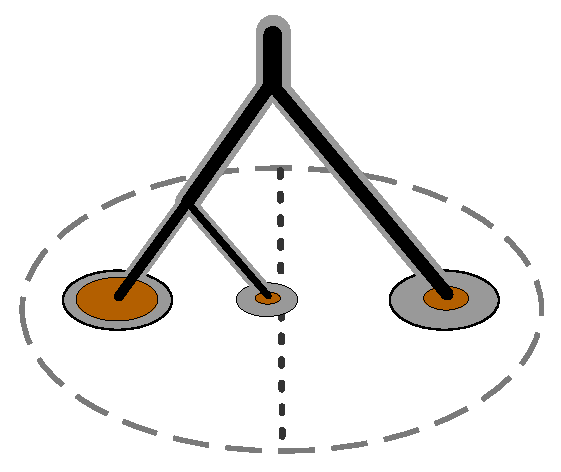
\includegraphics[width=.4\textwidth]{figures/piranha/cartoons/angular_discont_left}
          \label{fig:ang_discont_left}
      }
      ~~~~
      \subfloat[]{
          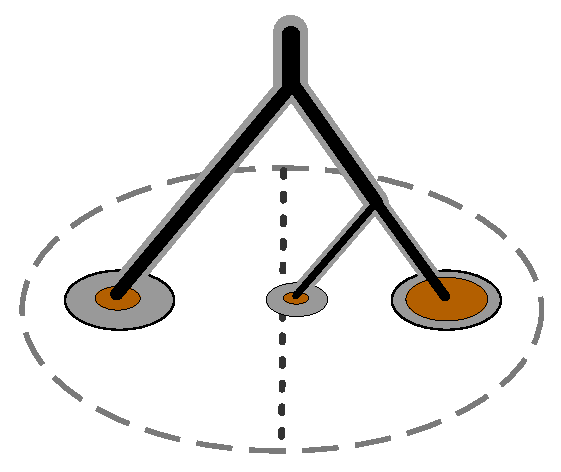
\includegraphics[width=.4\textwidth]{figures/piranha/cartoons/angular_discont_right}
          \label{fig:ang_discont_right}
      }
      \caption[A visualization of angular discontinuity in tree-based grooming.]{
    A visualization of angular discontinuity in tree-based grooming in the style of \Fig{rsf_tree}, with the angular-ordered \PRSF{1/2} algorithm as a representative example.
    %
    The thick dashed line in the center of the jet is equidistant in angle from the left and right sub-jets of the event, and the middle emission lies nearly on this line.
    %
    In (a), the middle emission lies closer to the left sub-jet, and the right sub-jet is therefore groomed more.
    %
    In (b), the middle emission is closer to the right sub-jet, and the left sub-jet is groomed more.
    %
    We see that a small change in the angle of the middle emission may drastically change the clustering history of the jet, and the result of a tree-based grooming procedure.
}
\label{fig:angdiscont}
\end{figure}


In our discussion, we focus on a simple manifestation of angular clustering discontinuities in the three-parton jet shown in \Fig{angdiscont}.
%
In particular, we consider the region of phase space where a particular sub-jet is nearly equidistant from a sub-jet on the left and another on the right.
%
We call the left and right sub-jets \(L\) and \(R\), and we denote the equidistant emission as \(M\), for ``middle''.

A small change in the location of emission \(M\) may lead to distinct C/A clustering histories.
%
If \(M\) is slightly closer to the left emission \(L\), then \(L\) will receive a quarter of the total grooming while \(R\) will receive half (as in \Fig{ang_discont_left});
%
the result is that \(L\) is groomed less than \(R\), and much more of the structure of the left side of the jet is preserved after the grooming.
%
Alternatively, if \(M\) is slightly closer to the right, then \(R\) will be groomed less than \(L\);
%
the right side of the jet will be preserved while much of the left side will be groomed away (as in \Fig{ang_discont_right}).
%
Despite the similarity of the ungroomed events, the resulting groomed events will have macroscopic differences and be separated by a relatively large EMD.

To emphasize this point quantitatively, let us consider P-RSF acting on the simple example where all three emissions lie in a plane, the left and right emissions each have an energy fraction \(z_\ell = z_r = z_0\), and the middle emission -- nearly equidistant from the left and right emissions -- has \(z_m = 1-2z_0\).\footnote{We focus on P-RSF in this example to avoid the more complex analysis required for Soft Drop that may obfuscate the physics at hand.
%
Soft Drop also exhibits an angular clustering discontinuity that can be seen in the context of this simple example, but that is complicated by the possible behaviors of the grooming:
%
\(\zcut\) and \(z_0\) may conspire such that zero, one, or two emissions are groomed from the event.
%
The effects of the clustering discontinuity on the energy-weighted jet axis must therefore be considered piece-wise in the \((\zcut,\,z_0)\) parameter space.
}
%
We use \(R\) to denote the angle between the left and right emissions, and \(\delta\) to denote a small perturbation in the angle of the middle emission:
%
\(\theta_{\ell m} = R/2 + \delta\) in one event, while \(\theta_{\ell m} = R/2 - \delta\) in the other.
%
We again examine the discontinuity in the energy-weighted jet axis, which takes the more general form
\begin{align}
    \hat{n}_{\rm jet} \propto \sum_i z_i \hat{n}_i
    ,
\end{align}
where the proportionality holds up to normalization.
%
A simple computation then yields
\begin{subequations}
\begin{align}
    \Delta\theta_0
    &=
    2\, z_m \, \delta
    +
    \mathcal{O}\left(R^2, \delta^3\right)
    ,
    \\
    \lim_{\delta\to 0}\Delta\theta_0 &= 0
    ,
\end{align}
\end{subequations}
for the angle \(\Delta\theta_0\) between the two jet axes before grooming, while
\begin{align}
    \lim_{\delta\to 0}\Delta\theta_g
    &=
    R\,\frac{\zcut}{1-\zcut}\,\left|f(f-3)+1\right|
    +
    \mathcal{O}(R^3)
    \neq 0
    ,
\end{align}
for the angle between the two jet axes after the application of P-RSF, where we have assumed that \(\zcut\) is sufficiently small that all particles survive the grooming.
%
We again see a discontinuous behavior in the energy-weighted axis of the groomed jets, \(\lim_{\delta\to 0}\Delta\theta_g \neq 0\), despite the fact that the ungroomed events were nearly identical and \(\lim_{\delta\to 0}\Delta\theta_0 = 0\).


Fortunately, the angular discontinuities associated with tree-based clustering algorithms are also suppressed in the phase space of \gls{pqcd}.
%
First, we note that the angular discontinuities in angular-ordered clustering algorithms emerge only at higher orders of perturbative accuracy for which a jet has three or more constituents.
%
These regions of phase space are generically suppressed in high-energy QCD calculations, where the emission of extra final-state partons is suppressed by the strong coupling constant \(\alpha_s\).
%
Furthermore, \gls{pqcd} predicts a strong hierarchy in the angles between different emissions in a jet, \(\theta_1 \gg \theta_2 \gg \cdots\) \cite{Collins:2011zzd}.
%
Therefore, even among phase space configurations with three or more constituents, it is very unlikely in \gls{pqcd} to find a configuration in which a particular final-state particle lies nearly equidistant in angle between two others.

We also emphasize that the angular discontinuity of the C/A clustering algorithm is representative of more general discontinuities in tree-based clustering and in jet algorithms.\footnote{
To mitigate the discontinuities of tree-based clustering, one can introduce a continuous weighting procedure for clustering histories.
%
One way to assign continuous weights to different clustering histories is the \textsc{Q-jet} scheme \cite{Ellis:2012sn,Ellis:2014eya}, which notably leads to reduced statistical fluctuations in observable distributions compared to the standard scheme of using a single clustering history for jet substructure calculations.
%
While the \textsc{Q-jet} scheme has not been applied directly to grooming in the context of energy flows, to our knowledge, it provides a particularly simple way to overcome the clustering discontinuities we discuss here:
%
we may simply define an overall groomed energy flow -- devoid of clustering discontinuities -- as the weighted average of the groomed energy flows associated with each possible clustering history.
}
%
For example, the \(k_t\) and anti-\(k_t\) algorithms exhibit a similar \(k_t\) discontinuity by identical arguments.
%
Discontinuities of different clustering algorithms may be more or less suppressed in the phase space of \gls{pqcd}, or more or less sensitive to particular sources of low-energy pollution.
%
Therefore, a more detailed discussion of clustering discontinuities and re-clustering schemes that minimize their effects is a potential direction for future research.


%==============================================
\section{Groomed Jet Phenomenology}
%==============================================
\label{sec:grooming-pheno}

We now demonstrate the soft insensitivity enjoyed by \PIRANHA{} groomers over hard-cutoff groomers through several phenomenological studies.
%
In \Secs{pira-hadronization}{pira-neutral}, we compare the responses of the hard-cutoff Soft Drop algorithm and \PRSF{1/2} to \glspl{soft-distortion} from \gls{hadronization} and to the removal of neutral particles, as a proxy for \gls{deteffects}.
%
In \Secss{pira-pu}{pira-ue}{pira-mass}, we compare the ability of Soft Drop and \PRSF{1/2} to effectively remove \gls{additive-contamination} from \gls{pileup} and \gls{ue}, which both consist of \textit{extra} soft radiation that sits on top of a hard process.
%
In particular,
\begin{itemize}
    \item
        We use \PRSF{1/2} as a representative of \PIRANHA{} grooming procedures;

    \item
        We use Soft Drop with \(\beta_{\rm SD} = 2\) as a representative of traditional grooming procedures.

    \item
        In our \gls{pileup} studies, we use Constituent Subtraction (CS), a constituent-level area subtraction method for \gls{pu-mitigation} \cite{Berta:2014eza}, as a representative of \gls{pileup} mitigation procedures.
\end{itemize}
%
We also present more detailed phenomenological comparisons of \PIRANHA{} and \glslink{hard-cutoff-groomer}{hard-cutoff grooming algorithms} in \App{feedingfrenzy}


The case of \gls{additive-contamination} is qualitatively different than that of \glspl{soft-distortion};
%
we do not want to examine the robustness of the grooming procedure to \gls{additive-contamination}, but rather the ability of the grooming to \textit{remove} the contamination.
%
In our \gls{pileup} mitigation studies, we find that \PRSF{1/2} -- which behaves comparably to CS -- is a more effective tool than \SD{2}.
%
In our \gls{ue} studies, we find that \PRSF{1/2} and \SD{2} are comparable tools for the subtraction of \gls{ue} effects from jet substructure.

We simulate \gls{pileup} using the dijet and minimum bias samples from \Reff{Soyez:2018opl}, produced using \texttt{Pythia 8.185} with tune 4C for proton-proton collisions at \(\sqrt{s}\) = 14 TeV.
%
We layer minimum bias events on top of the hard dijet events, taking the number of \glslink{pileup}{pileup} events to be Poisson distributed with a mean of \(\langle n_{\rm PU}\rangle\) = 50 events.

We simulate \gls{ue} by turning on multiple parton interactions in \texttt{Pythia 8.244} \cite{Sjostrand:2014zea} with the default Monash tune \cite{Skands:2014pea}.
%
We begin with a study of QCD jets and, to roughly echo similar studies in the original Soft Drop paper \cite{Larkoski:2014wba}, also explore the groomed mass resolution of jets produced by boosted \(W\) bosons and top quarks in the presence of \gls{ue}.

For details regarding other \PIRANHA{} grooming procedures and Soft Drop with different \(\beta_{\rm SD}\), see \App{feedingfrenzy}.




%=====================================
% Hadronization:
%=====================================
\subsection{Hadronization Response}
\label{sec:pira-hadronization}

We first provide phenomenological evidence that continuous grooming is less sensitive than hard-cutoff grooming to the physics of \gls{hadronization}.
%
A deep understanding of the physics of traditional jets requires careful consideration of \gls{hadronization} corrections, such as in jet masses \cite{Hoang:2019ceu, Marzani:2017kqd, Benkendorfer:2021unv} and hadronic event shapes \cite{Dokshitzer:1995zt, Baron:2020xoi}.
% and we hope that \PIRANHA{} grooming provides observables that may be more easily understood without complicated non-perturbative input.
%
Hard-cutoff groomed jet observables in particular can undergo large corrections from the \gls{hadronization} process due to the discontinuity of the hard-cutoff paradigm:
%
\gls{hadronization} can transform partons with energy below a hard cutoff into hadrons with energy above the hard cutoff, and vice versa.
%
These subtleties lead to additional complications in the theoretical calculation of non-perturbative effects on traditionally groomed jet observables \cite{Hoang:2019ceu}.

%-----------------------------------
% Parton-Hadron EMD:
%-----------------------------------
\begin{figure}[p]
\centering
\subfloat[][]{
      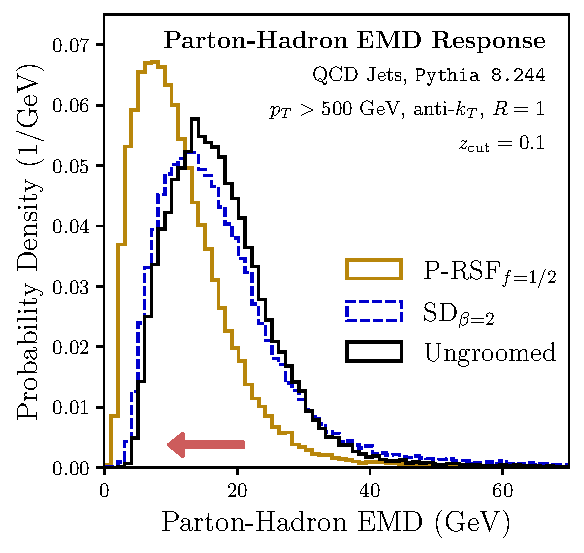
\includegraphics[width=.32\textwidth]
      {figures/piranha/responses/pvh/emd_dist-ph}
      \label{fig:ph_emd_dist}
}
\subfloat[][]{
      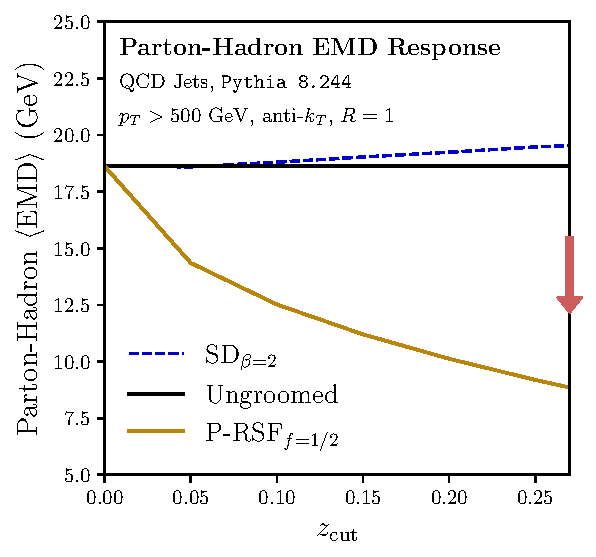
\includegraphics[width=.32\textwidth]
      {figures/piranha/responses/pvh/deltaemd-ph}
      \label{fig:ph_emd_delta}
}
\subfloat[][]{
      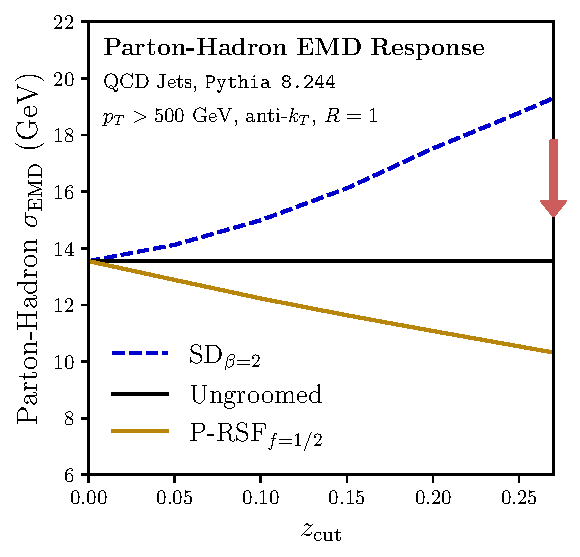
\includegraphics[width=.32\textwidth]
      {figures/piranha/responses/pvh/sigmaemd-ph}
      \label{fig:ph_emd_sigma}
}
\\
\subfloat[][]{
      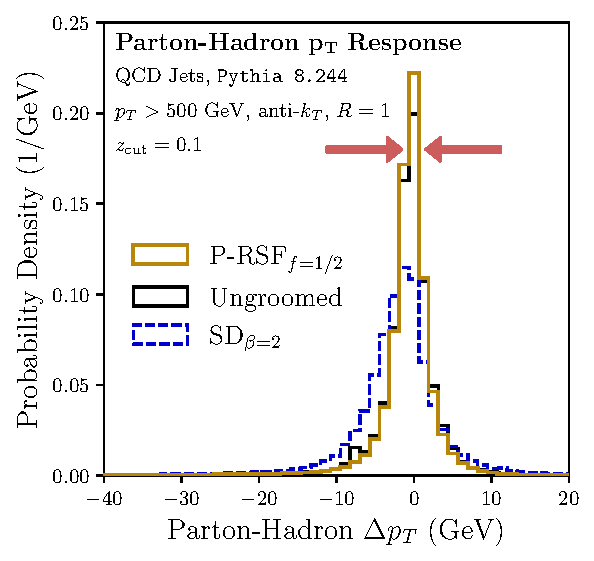
\includegraphics[width=.32\textwidth]
      {figures/piranha/responses/pvh/delta_pt_dist-ph}
      \label{fig:ph_pt_dist}
}
\subfloat[][]{
      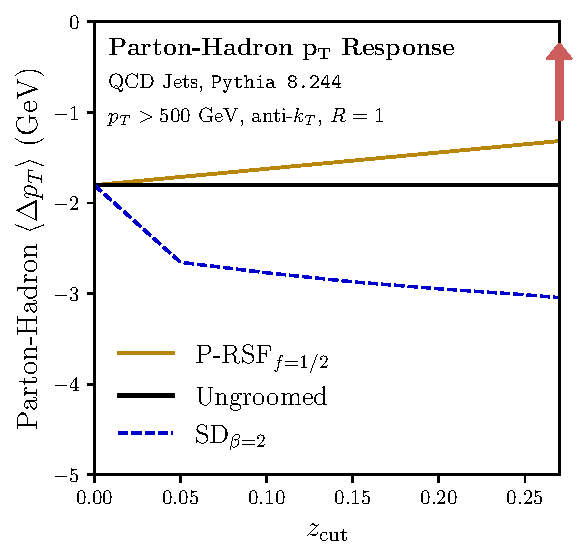
\includegraphics[width=.32\textwidth]
      {figures/piranha/responses/pvh/deltapt-ph}
      \label{fig:ph_pt_delta}
}
\subfloat[][]{
      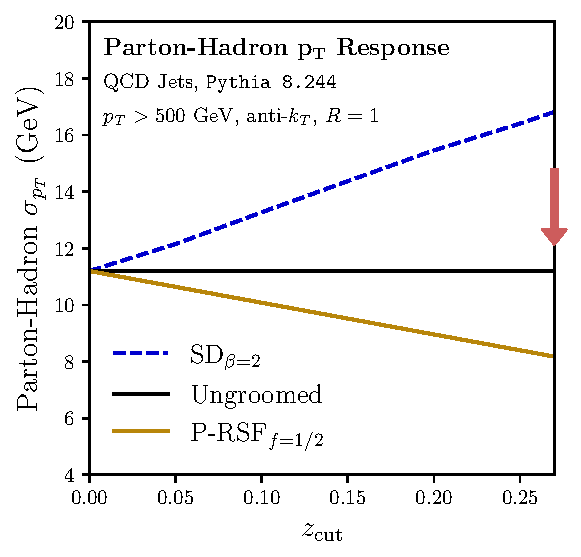
\includegraphics[width=.32\textwidth]
      {figures/piranha/responses/pvh/sigmapt-ph}
      \label{fig:ph_pt_sigma}
}
\\
\subfloat[][]{
      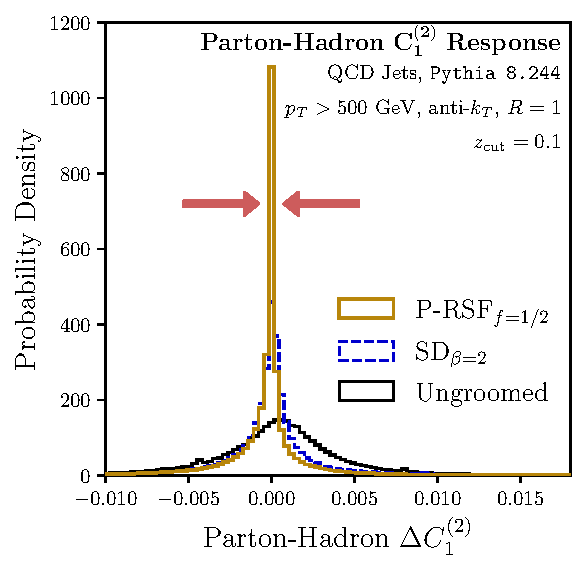
\includegraphics[width=.32\textwidth]
      {figures/piranha/responses/pvh/deltac12_dist-ph}
      \label{fig:ph_c12_dist}
}
\subfloat[][]{
      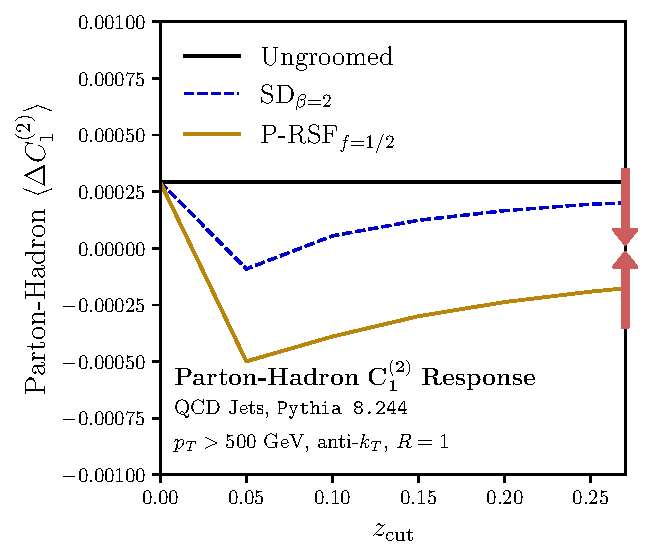
\includegraphics[width=.32\textwidth]
      {figures/piranha/responses/pvh/deltac12-ph}
      \label{fig:ph_c12_delta}
}\subfloat[][]{
      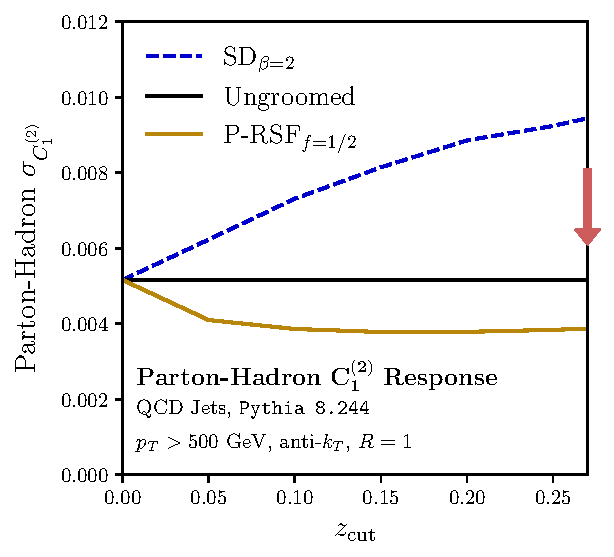
\includegraphics[width=.32\textwidth]
      {figures/piranha/responses/pvh/sigmac12-ph}
      \label{fig:ph_c12_sigma}
}
    \caption[Per-jet hadronization responses of the EMD, \(\Delta p_T\), and \(\Delta C_1^{(2)}\) using Balanced Recursive Subtraction and Soft Drop with \(\beta_{\rm SD} = 2\).]{
        Per-jet \gls{hadronization} responses of (top row) EMD, (middle row) \(\Delta p_T\), and (bottom row) \(\Delta C_1^{(2)}\) using Balanced Recursive Subtraction (\PRSF{1/2}, orange) and Soft Drop with \(\beta_{\rm SD} = 2\) (\SD{2}, blue).
        %
        We display (left column) the distribution of the response for \zcut=0.1, (middle column) the mean response as a function of \zcut, and (right column) the standard deviation of the response as a function of \zcut.
    %
    The red arrows indicate the direction corresponding to better performance.
    }
\label{fig:parton_hadron_response}
\end{figure}

In \Fig{parton_hadron_response}, we compare how ungroomed jets, traditionally groomed jets, and \PIRANHA{}-groomed jets respond to \gls{hadronization} in the context of energy flow, extensive properties, and substructure.
%
Our studies focus on the parton-hadron EMD (the EMD between parton-level jets and their hadron-level counterparts), the parton-hadron \(\Delta p_T\), and the parton-hadron \(\Delta C_1^{(2)}\).
%
\PIRANHA{}-groomed jets typically exhibit smaller and more predictable responses to \gls{hadronization}, evinced by the reduced variance in their \gls{hadronization} response.
%
One key factor in the improved responses of \PIRANHA{}-groomed jets is the scaling-down of distortions due to \gls{hadronization} in \PIRANHA{}-groomed jets:
%
the subtractive approach of \PIRANHA{} (and in particular P-RSF when \(f_{\rm soft} \neq 0, 1\)) removes energy from every particle in the event, resulting in a controlled and uniform \gls{hadronization} response.
%
On the other hand, Soft Drop grooming does not implement continuous, event-wide subtraction.
%
Jets groomed with Soft Drop either retain or remove particles as a result of distortions due to \gls{hadronization}, resulting in a larger variance in the properties of jets groomed with Soft Drop.

We plot distributions of the parton-hadron EMD for groomed QCD jets for the benchmark value of $\zcut{}=0.1$ in \Fig{ph_emd_dist}.
%
We see a sharper peak at a smaller EMD in the parton-hadron EMD distributions for \PRSF{1/2} and longer tails for Soft Drop, already indicating that \gls{hadronization} is more likely to dramatically change the result of Soft Drop.
%
\Figs{ph_emd_delta}{ph_emd_sigma} show that the average parton-hadron EMD and the variance in the parton-hadron EMD are both smaller for \PRSF{1/2} groomed jets than for Soft Drop groomed jets for a wide range of \zcut{} values, again evincing that \PIRANHA{}-groomed jets have less sensitive responses to \gls{hadronization}.


The extensive observable \(p_T\) and the substructure observable \(C_1^{(2)}\) also reflect the increased robustness of \PIRANHA{}-groomed jets to \gls{hadronization}.
%
In our discussion of \gls{hadronization}, we characterize the response of \(p_T\) by using \Eq{pt_response} with \(p_T = p_T^{\rm(parton)}\) indicating the parton-level transverse momentum, before the addition of model-dependent \gls{hadronization} effects, and \(\widetilde{p_T} = p_T^{\rm(hadron)}\).
%
In \Fig{ph_pt_dist}, we see that for \(\zcut = 0.1\), \PIRANHA{}-groomed \(p_T\) again tends to have a sharper response to \gls{hadronization}, while \Figs{ph_pt_delta}{ph_pt_sigma} indicates that this sharper response holds for a wide range of \zcut{} values.
%
The behavior of the \(p_T\) closely mimics that of the parton-hadron EMD, evincing our arguments that the parton-hadron EMD provides a probe of generic jet observables to \gls{hadronization}.
%
In \Figss{ph_c12_dist}{ph_c12_delta}{ph_c12_sigma}, we make similar conclusions for \(C_1^{(2)} \approx m^2 / p_T^2\).
%
We first note that the parton-hadron shift in the \(C_1^{(2)}\) substructure observable is larger for \PRSF{1/2}, at least for fixed \zcut{}, and the substructure of \PRSF{1/2} groomed jets may undergo larger changes due to \gls{hadronization} than that of Soft Drop groomed jets.
%
However, the variance in the shift in \PRSF{1/2} groomed substructure is smaller than that of Soft Drop, indicating that the response of \PIRANHA{}-groomed substructure to \gls{hadronization} is more predictable than that of Soft Drop.

Overall, we find that \PIRANHA{}-groomed jets have more predictable responses to \gls{hadronization} than traditionally groomed jets, supported by the observable independent EMD, as well as by extensive observables and jet substructure.
%
We have provided evidence that IRC-safe observables of jets groomed with Soft Drop have generically larger responses to \gls{hadronization}, while \PIRANHA{}-groomed observables are generally less affected by the physics of \gls{hadronization}.
%
We hope that the stability of \PIRANHA{}-groomed jets to the non-perturbative physics of \gls{hadronization} may facilitate even further communication between theoretical predictions and experimental results for groomed jet observables.

%=====================================
% All vs. Charged:
%=====================================
\subsection{All Versus Charged}
\label{sec:pira-neutral}

%-----------------------------------
% All-Charged EMD:
%-----------------------------------
\begin{figure}[p]
    \subfloat[][]{
          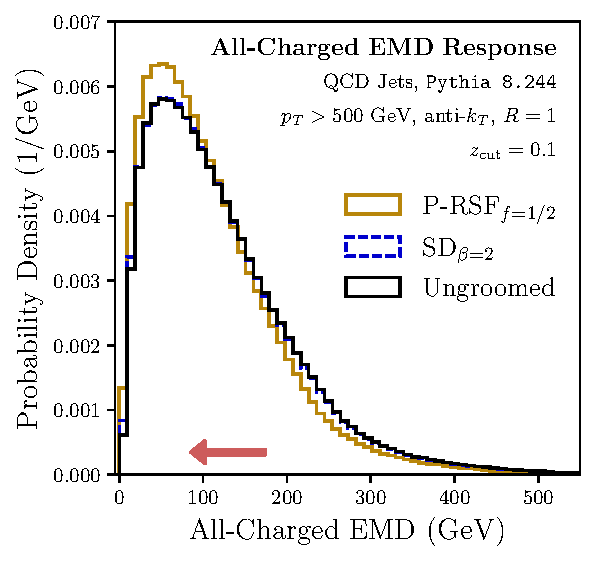
\includegraphics[width=.32\textwidth]
          {figures/piranha/responses/avc/emd_dist-avc}
          \label{fig:avc_emd_dist}
    }
    \subfloat[][]{
          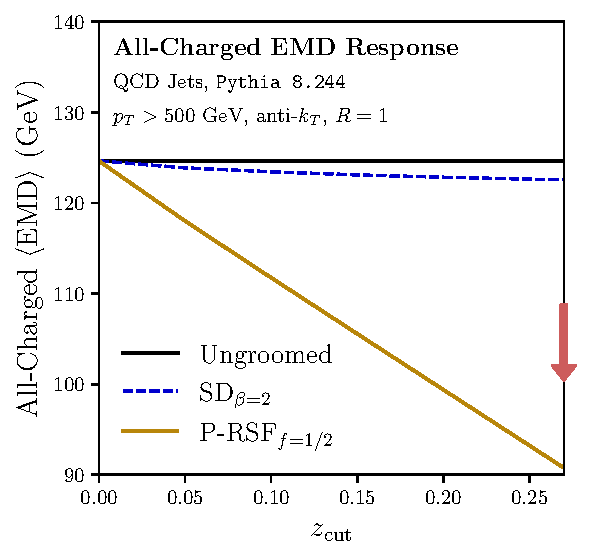
\includegraphics[width=.32\textwidth]
          {figures/piranha/responses/avc/deltaemd-avc}
          \label{fig:avc_emd_delta}
    }
    \subfloat[][]{
          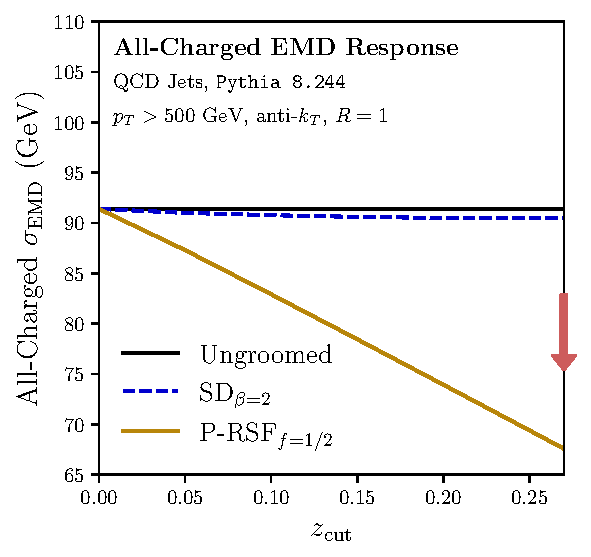
\includegraphics[width=.32\textwidth]
          {figures/piranha/responses/avc/sigmaemd-avc}
          \label{fig:avc_emd_sigma}
    }
    \\
    \subfloat[][]{
          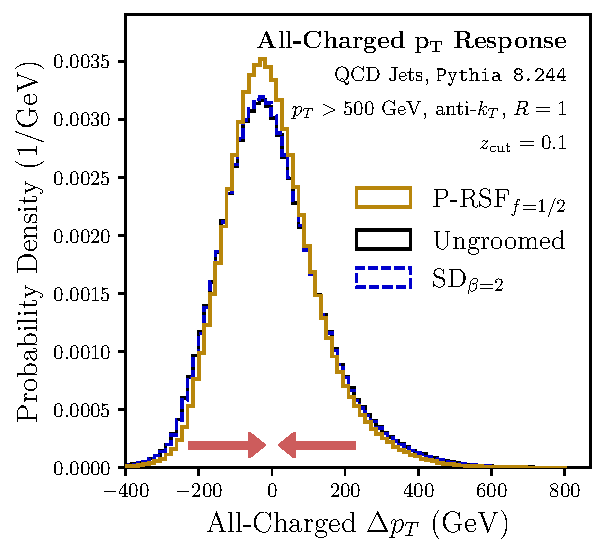
\includegraphics[width=.32\textwidth]
          {figures/piranha/responses/avc/delta_pt_dist-avc}
          \label{fig:avc_pt_dist}
    }
    \subfloat[][]{
          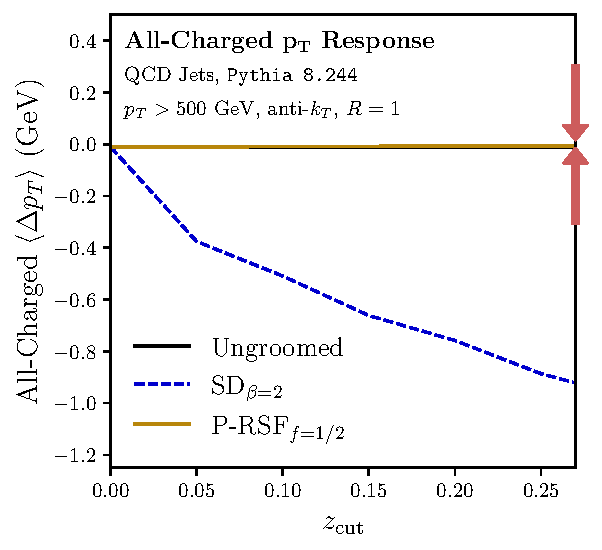
\includegraphics[width=.32\textwidth]
          {figures/piranha/responses/avc/deltapt-avc}
          \label{fig:avc_pt_delta}
    }
    \subfloat[][]{
          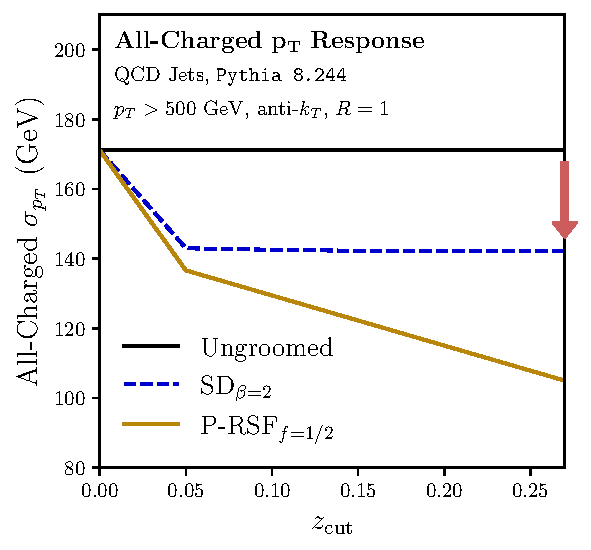
\includegraphics[width=.32\textwidth]
          {figures/piranha/responses/avc/sigmapt-avc}
          \label{fig:avc_pt_sigma}
    }
    \\
    \subfloat[][]{
          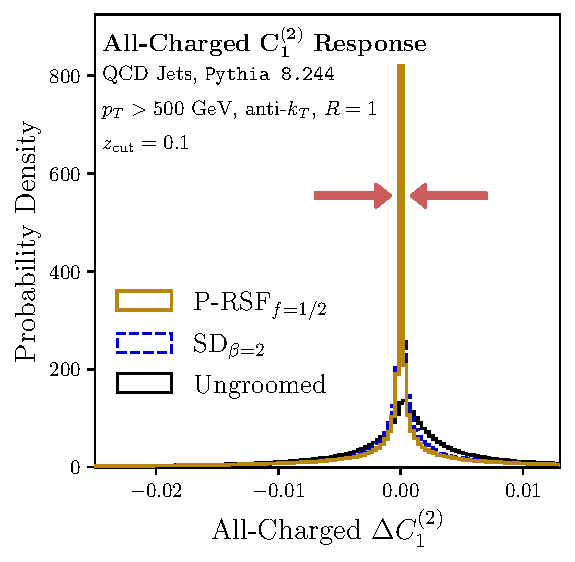
\includegraphics[width=.32\textwidth]
          {figures/piranha/responses/avc/deltac12_dist-avc}
          \label{fig:avc_c12_dist}
    }
    \subfloat[][]{
          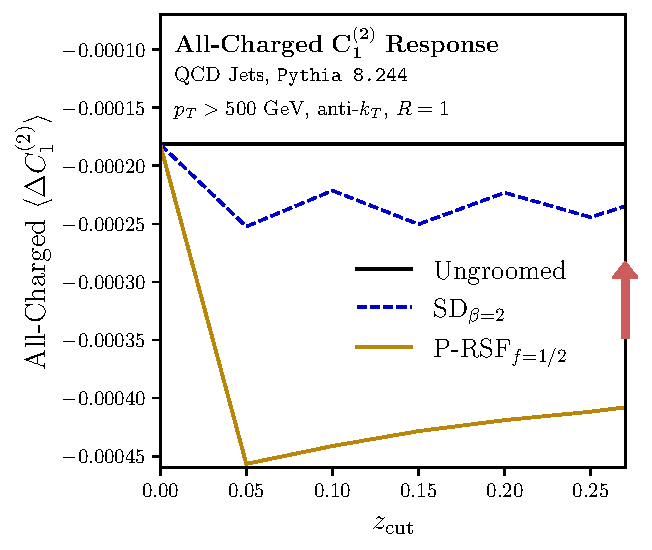
\includegraphics[width=.32\textwidth]
          {figures/piranha/responses/avc/deltac12-avc}
          \label{fig:avc_c12_delta}
    }
    \subfloat[][]{
          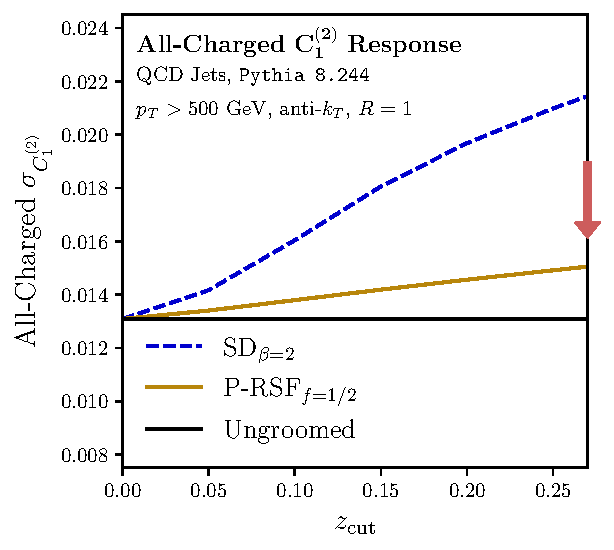
\includegraphics[width=.32\textwidth]
          {figures/piranha/responses/avc/sigmac12-avc}
          \label{fig:avc_c12_sigma}
    }
\caption[Responses to the exclusion of neutral particles of the EMD, \(\Delta p_T\), and \(\Delta C_1^{(2)}\) using Balanced Recursive Subtraction and Soft Drop with \(\beta_{\rm SD} = 2\).]{
    Same as \Fig{parton_hadron_response}, but for per-jet responses to the exclusion of neutral particles.
    %
    We rescale the \(p_T\) of the charged particles in order to eliminate the leading $p_T$ bias due to the loss of neutral energy.
}
\centering
\label{fig:avc_response}
\end{figure}

We next compare the response of hard-cutoff and \PIRANHA{} grooming to the exclusion of neutral particles, as a rough analog of the smearing of neutral particles due to \gls{deteffects}.
%
Small tweaks in experimental signatures due to \gls{deteffects} may produce large changes in hard-cutoff groomed observables, providing another obstacle in extracting fundamental physics from traditionally groomed jets.
%
The continuity of \PIRANHA{} again leads us to expect that \PIRANHA{}-groomed observables are more robust to \gls{deteffects} than traditionally groomed jet observables.


To counteract the leading bias due to the loss of neutral energy in the jet, we apply a rescaling to the \(p_T\) of the charged-only jet constituents:
%
\begin{align}
    \tilde p_T^i =
    \begin{cases}
        0,
        &\text{particle }i\text{ is neutral}
        \\
        p_T^i
        \frac{\left\langle p_T^\text{(all)}\right\rangle}{\left\langle p_T^\text{(charged)}\right\rangle},
        &\text{particle }i\text{ is charged}
    \end{cases}
    ,
    \label{eq:all-charged_rescaling}
\end{align}
where \(p_T^i\) is the transverse momentum of particle \(i\) in the original jet, \(\mathcal{J}\), containing both charged and neutral particles, and \(\tilde p_T^i\) is the transverse momentum we assign to particle \(i\) in the charged-only, rescaled jet, \(\tilde{\mathcal{J}}\), with neutral particles excluded.
%
Here, \(p_T^{\rm(all)} = \sum_i p_T^i\) is the total transverse momentum including both charged and neutral particles, while \(p_T^{\rm(charged)} = \sum_{i\text{ charged}} p_T^i\) includes only charged constituents.
%
The rescaling factor \(\big\langle p_T^\text{(all)}\big\rangle/\big\langle p_T^\text{(charged)}\big\rangle\)\(\approx\)\(1.47\) is defined such that the average $p_T$ is preserved after removing neutral particles.%
\footnote{
We can gain intuition for this rescaling factor by considering the isospin-preserving limit, where we expect similar numbers of \(\pi^+\), \(\pi^-\), and \(\pi^0\) mesons to be produced.
%
Events for which we discard the \(\pi^0\) particles should have roughly \(2/3\) the total transverse momentum, ignoring subtleties associated with kaons and other heavier states.
%
This leads to an estimate of \(\big\langle p_T^\text{(all)}\big\rangle/\big\langle p_T^\text{(charged)}\big\rangle \approx 3/2\) -- remarkably close to the numerical value of 1.47 found in \texttt{Pythia 8.244}.
}

In our discussion of EMD, we compute the response \(\text{EMD}\left(G(\mathcal{J}), G(\tilde{\mathcal{J}})\right)\), where \(G\) indicates the grooming algorithm under consideration;
%
we call this the \textit{all-charged EMD}.
%
Similarly, in our discussion of \Eq{pt_response}, we take \(p_T = p_T^{\rm(all)}\) to be the transverse momentum including both charged and neutral particles and \(\widetilde{p_T} = \sum_i \tilde p_T^i = p_T^{\text{(charged, rescaled)}}\) to be the rescaled contribution from charged particles only.
%
We refer to the difference as the all-charged \(p_T\) shift, or the all-charged \(\Delta p_T\).
%
Note that the rescaling procedure does not impact dimensionless charged-only substructure observables like \(C_1^{(2)}\), since they are normalized by the jet momentum.


Our comparison of the all-charged response of \PIRANHA{} grooming to that of traditional grooming procedures is shown in \Fig{avc_response}.
%
As in our study of \gls{hadronization}, we begin our study with a discussion of the EMD.
%
The all-charged EMD bounds changes in IRC-safe observables due to the exclusion of neutral particles and corresponding rescaling of charged particles.
%
Since neutral particles are the most susceptible to smearing effects due to detector responses, the all-charged EMD furnishes an observable-independent probe for the effects of experimental detectors on groomed jets.
%
We demonstrate distributions of the all-charged EMD for groomed QCD jets with several choices of grooming in \Fig{avc_emd_dist}.
%
The contrast between \PIRANHA{} and traditionally groomed all-charged EMD is not as sharp as for the parton-hadron EMD.
%
However, \PIRANHA{} grooming again enjoys smaller and more sharply peaked EMD responses to the exclusion of neutral particles.
%
\Fig{avc_emd_delta} shows that the all-charged EMD is smaller for P-RSF\(_{1/2}\) groomed jets than for Soft Drop groomed jets for a wide range of \zcut{} values.
%
\Fig{avc_emd_sigma} shows that the fluctuations in the all-charged EMD, and therefore the fluctuations in the response of grooming to our naive model of smearing, are noticeably smaller for \PIRANHA{} groomers than for traditional groomers.

Our results for the all-charged \(p_T\) shifts are similar to our results for the all-charged EMD.
%
\Fig{avc_pt_dist} demonstrates that the \(p_T\) response of \PRSF{1/2} is smaller and more sharply peaked for $\zcut = 0.1$, while \Figs{avc_pt_delta}{avc_pt_sigma} respectively show that the \PRSF{1/2} all-charged response remains small and sharply peaked for a wide range of \zcut{} values.
%
Indeed, the fluctuations of the all-charged \(p_T\) response are nearly identical for each \PIRANHA{} groomer.

\Figss{avc_c12_dist}{avc_c12_delta}{avc_c12_sigma} compare the robustness of \PRSF{1/2} and Soft Drop for the substructure observable \(C_1^{(2)}\).
%
\Fig{avc_c12_dist} again shows that the all-charged response of \PRSF{1/2} is more sharply peaked than that of Soft Drop.
%
Similarly, \Figs{avc_c12_delta}{avc_c12_sigma} demonstrate that the all-charged shifts to \PIRANHA{}-groomed jet substructure are generally larger but more predictable than those of Soft Drop for a wide range of \zcut{} values.
%
The increased robustness of \PIRANHA{} grooming procedures compared to Soft Drop is less sharp than in the case of \gls{hadronization}, but the \PIRANHA{}-groomed observables nonetheless have less spread and a stronger linear correlation in response to our naive model of smearing.


%=====================================
% Pileup:
%=====================================
\subsection{Minimum Bias Events and Pileup Response}
\label{sec:pira-pu}

%-----------------------------------
% Pileup:
%-----------------------------------
\begin{figure}[p]
\centerline{
\subfloat[][]{
      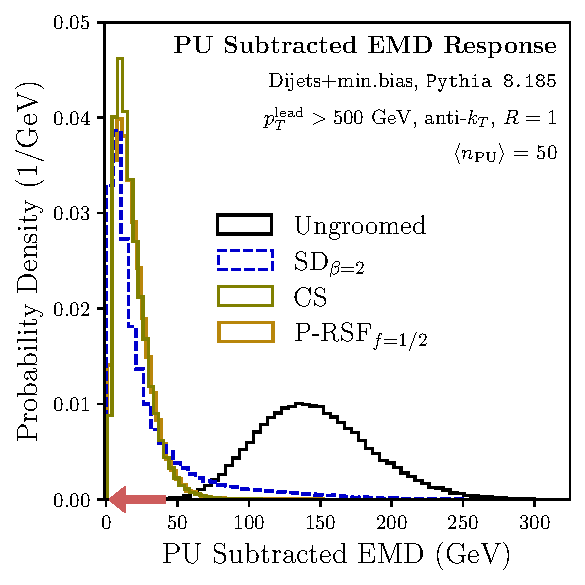
\includegraphics[width=.32\textwidth]{figures/piranha/responses/pileup/main_emd_npu50}
      \label{fig:pu_emd_dist}
}
\subfloat[][]{
      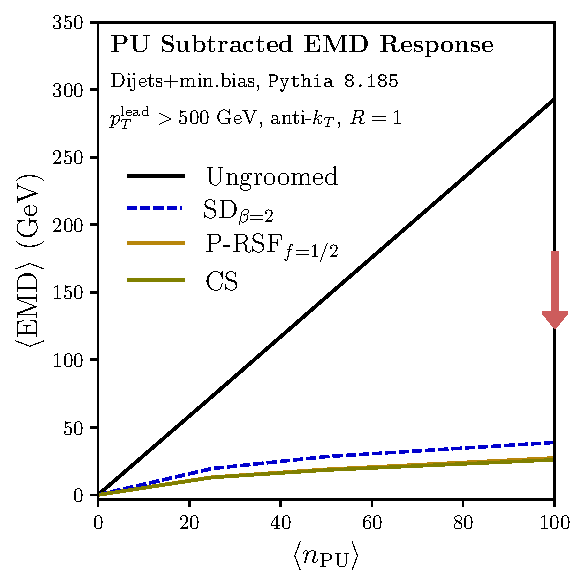
\includegraphics[width=.32\textwidth]{figures/piranha/responses/pileup/main_emd_npu_shifts}
      \label{fig:pu_emd_shift}
}
\subfloat[][]{
      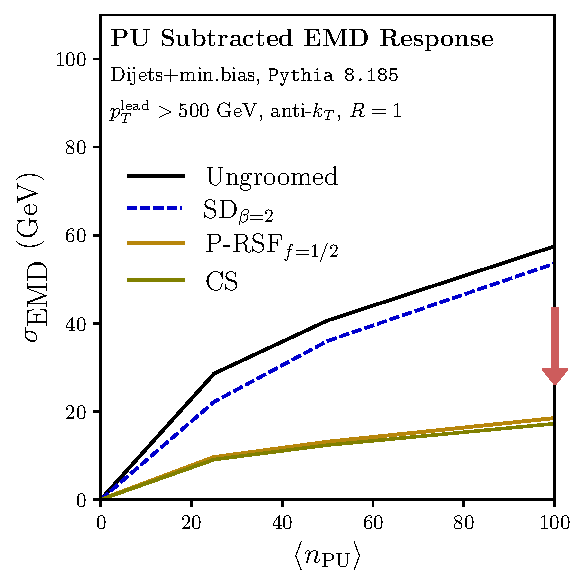
\includegraphics[width=.32\textwidth]{figures/piranha/responses/pileup/main_emd_npu_stds}
      \label{fig:pu_emd_std}
}
} % centerline
~\\
\centerline{
\subfloat[][]{
      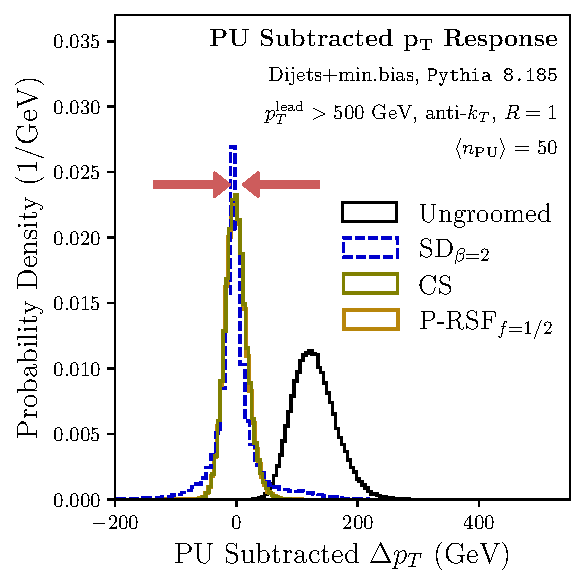
\includegraphics[width=.32\textwidth]{figures/piranha/responses/pileup/main_dpt_npu50}
      \label{fig:pu_pt_dist}
}
\subfloat[][]{
      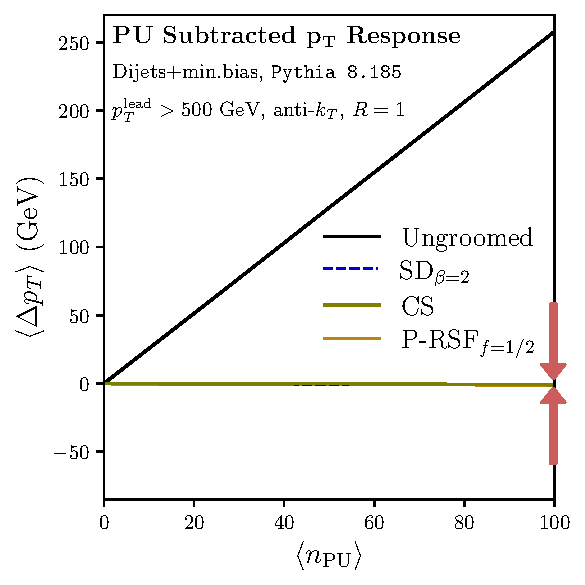
\includegraphics[width=.32\textwidth]{figures/piranha/responses/pileup/main_dpt_npu_shifts}
      \label{fig:pu_pt_shift}
}
\subfloat[][]{
      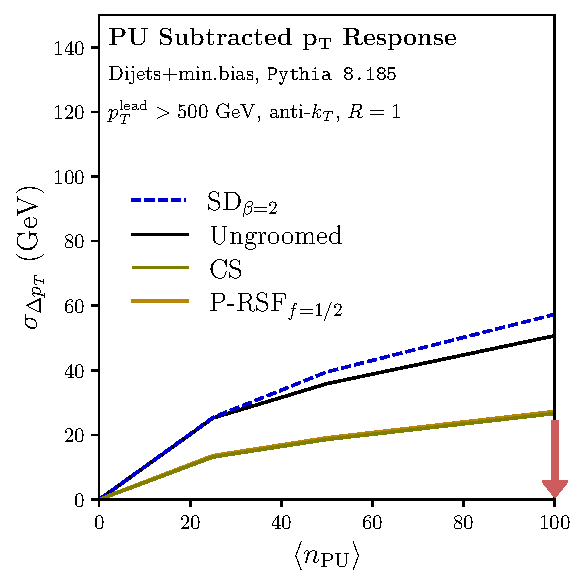
\includegraphics[width=.32\textwidth]{figures/piranha/responses/pileup/main_dpt_npu_stds}
      \label{fig:pu_pt_std}
}
} % centerline
~\\
\centerline{
\subfloat[][]{
      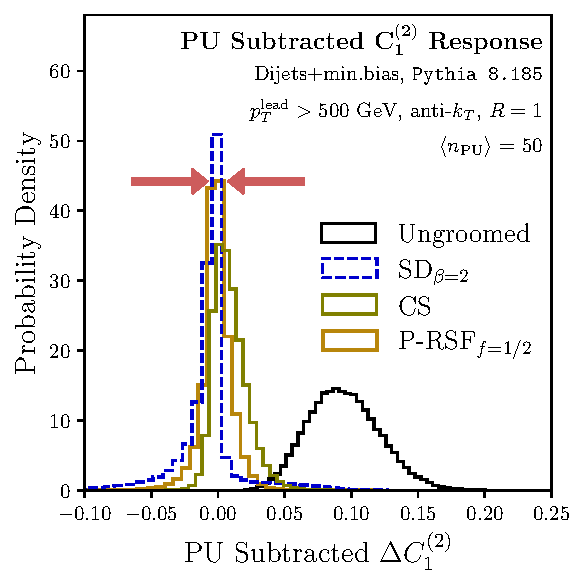
\includegraphics[width=.32\textwidth]
      {figures/piranha/responses/pileup/main_dc1_npu50}
      \label{fig:pu_c12_dist}
}
\subfloat[][]{
      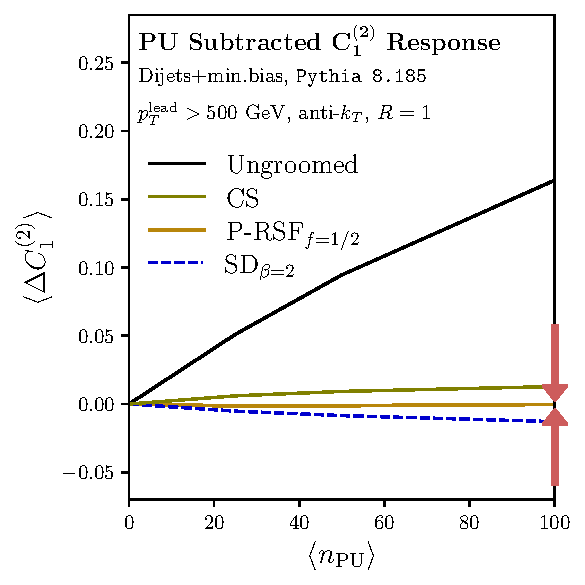
\includegraphics[width=.32\textwidth]
      {figures/piranha/responses/pileup/main_dc1_npu_shifts}
      \label{fig:pu_c12_shift}
}
\subfloat[][]{
      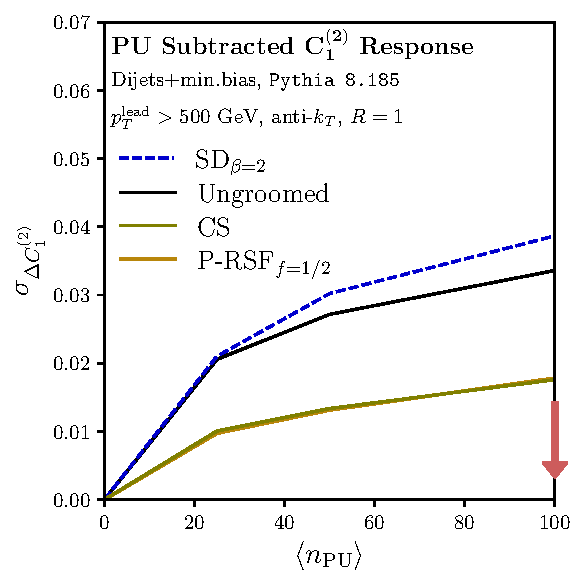
\includegraphics[width=.32\textwidth]
      {figures/piranha/responses/pileup/main_dc1_npu_stds}
      \label{fig:pu_c12_std}
}
} % centerline
\caption[Pileup-subtracted properties of the EMD, \(\Delta p_T\), and \(\Delta C_1^{(2)}\) using Balanced Recursive Subtraction and Soft Drop with \(\beta_{\rm SD} = 2\).]{
    Properties of per-jet \gls{pileup}-subtracted (top row) EMD, (middle row) \(\Delta p_T\), and (bottom row) \(\Delta C_1^{(2)}\), discussed in \Sec{pira-pu} for Balanced Recursive Subtraction (\PRSF{1/2}, orange), Soft Drop with \(\beta_{\rm SD} = 2\) (\SD{2}, blue), and Constituent Area Subtraction (CS, green).
    %
    We display (left column) the distribution of the each \gls{pileup}-subtracted observable for \(\langle n_{\rm PU}\rangle = 50\), (middle column) the mean \gls{pileup}-induced shift in each observable as a function of \(\langle n_{\rm PU}\rangle\), and (right column) the standard deviation of the \gls{pileup}-induced shifts in each observable as a function of \(\langle n_{\rm PU}\rangle\).
    %
    The red arrows indicate the direction corresponding to better performance.
}
\label{fig:pu_response}
\centering
\end{figure}

We first examine the effectiveness of different groomers in mitigating the effects of \gls{pileup} on the dijet events of \Reff{Soyez:2018opl}.
%
To quantify the ability of different groomers to remove \gls{pileup}, we perform an event-by-event comparison of \textit{hard events} to the associated \vocab{\glspl{pusubevent}}:
\begin{itemize}
    \item
    A \vocab{hard event} is a dijet event without any \gls{pileup}, representing the physics of a hard process;

    \item
    A \vocab{\gls{pusubevent}} is produced by simulating the \gls{additive-contamination} due to \gls{pileup} on top of a hard event and then attempting to groom the \gls{pileup} away.
\end{itemize}
%
To produce a \gls{pileup}-subtracted event, we first simulate \gls{pileup} by adding the energy distributions of a Poisson-distributed number of minimum bias events to the energy distribution of a given hard event.
    %
    We then estimate the contaminating energy density due to \gls{pileup} using the \texttt{GridMedianBackgroundEstimator} (GMBE) method of \texttt{FastJet} \cite{Cacciari:2011ma}.
    %
    We tune an additional correction factor that scales our estimate \(\rho_{\rm est.}\) relative to the GMBE value \(\rho_{\rm GMBE}\) for each grooming algorithm to subtract \glslink{pileup}{pileup} more effectively, as discussed in more detail in \App{feedingfrenzy}.
    %
    Finally, we produce the \gls{pusubevent} by removing a fraction \(\zcut\) of the jet \(p_T\) consistent with the estimated \glslink{pileup}{pileup} density:
\begin{align}
   \zcut\,p_T^{\rm(jet)}
   =
   \rho_{\rm est.}\,A_{\rm jet}
   \approx
   p_T^{\rm(PU~in~jet)}
   .
\end{align}

We examine the EMD, \(\Delta p_T\), and \(\Delta C_1^{(2)}\) between the \textit{leading jets} of the hard and \glslink{pileup}{pileup}-events in \Fig{pu_response}.\footnote{
In some situations, the \glslink{pileup}{pileup} contributes enough energy that the leading jet after the addition of \glslink{pileup}{pileup} corresponds to the direction of the sub-leading jet before the addition of \glslink{pileup}{pileup}.
%
This phenomenon occurs only for a small fraction of events, and we do not include these events in the following discussion.
}
%
In \Figss{pu_emd_dist}{pu_emd_shift}{pu_emd_std}, we examine the EMD between the leading jet in the hard dijet event and the leading jet in the subtracted event with \glslink{pileup}{pileup}.
%
\Fig{pu_emd_dist} demonstrates that when \(\langle n_{\rm PU} \rangle=50\), \PRSF{1/2} tends to subtract \glslink{pileup}{pileup} more accurately and predictably, evinced by a more sharply peaked EMD distribution and a smaller average \glslink{pusubevent}{PU-subtracted} EMD than found for CS and Soft Drop.
%
This strength of \PRSF{1/2} persists as the amount of \glslink{pileup}{pileup} is increased, as suggested by \Figs{pu_emd_shift}{pu_emd_std}.

\Figss{pu_pt_dist}{pu_pt_shift}{pu_pt_std} offer similar conclusions for the jet \(p_T\).
%
In our study of \glslink{pileup}{pileup} responses, \(p_T = p_T^{\rm(hard)}\) indicates the transverse momentum of the hard event, before the layering of minimum bias/pileup events, and \(\widetilde{p_T} = p_T^{\rm (groomed~PU)}\) indicates the transverse momentum after \glslink{pileup}{pileup} has been added and then groomed away.
%
RSF\(_{1/2}\) again reproduces the extensive quantity \(p_T\) of the jet in the absence of \gls{pileup} for a wide range of \(\langle n_{\rm PU} \rangle\) values.
%
Identical conclusions hold for the substructure of the jet, as suggested by the behavior of \(C_1^{(2)}\) shown in \Figss{pu_c12_dist}{pu_c12_shift}{pu_c12_std}.

\Figs{pufrenzy_ave}{pufrenzy_stddev} of \App{feedingfrenzy} evince further that with our tuned procedure for \gls{pileup} mitigation, \PIRANHA{} groomers and CS perform more reliably than traditional groomers in the removal of \glslink{pileup}{pileup}.
%
Furthermore, P-RSF algorithms are tree-based and offer orders-of-magnitude faster \gls{pileup} mitigation over CS, \gls{apollonius}, and \gls{ivs} (see \Fig{runtimes} of \App{feedingfrenzy}).


%=====================================
% Underlying Event:
%=====================================
\subsection{Underlying Event Response}
\label{sec:pira-ue}

We next examine the ability of grooming to eliminate \gls{additive-contamination} from \gls{ue}.
%
Since we model \gls{ue} by generating events in the presence of multiple parton interactions in \texttt{Pythia 8.244}, it is less straightforward to study the effects of \gls{ue} on an event-by-event basis.
%
We instead work at the level of \textit{distributions}:
%
we tune both \PRSF{1/2} and Soft Drop so that, when acting on events with \gls{ue}, they most accurately reproduce the substructure distribution of events without \gls{ue}.
%
We focus on substructure alone in our discussion of \gls{ue} correction because we cut on jets with \(p_T>500\) GeV both for events with and without \gls{ue}, and it is less meaningful to focus on the associated \(p_T\) distributions;
%
we leave a more detailed study of the ability of \PIRANHA{} groomers to remove \gls{ue} at an event-by-event level for future work.

We characterize the ability of groomers to correct for the presence of \gls{ue} by comparing \textit{base distributions} to \vocab{\glspl{ue-corrected}}:
\begin{itemize}
    \item
    A \vocab{base distribution} is a substructure distribution with a fixed grooming parameter, \(\zcut^{(\rm base)}\);

    \item
        A \vocab{\gls{ue-corrected}} is a substructure distribution in the presence of \gls{ue} and with slightly more grooming tuned to soak up the additional energy contribution from \gls{ue}:
    %
    \(\zcut^{(\rm corr.)} = \zcut^{(\rm base)} + \delta\zcut\).
\end{itemize}
We tune \(\delta \zcut\) by hand, for every \(\zcut^{(\rm base)}\), to optimally correct for the presence of \gls{ue}\footnote{
We note that the optimized \(\delta\zcut\) is energy-dependent and process-dependent.
%
For example, we expect that \(\delta\zcut\) should be parametrically smaller for processes at higher energies since the energy removed from a jet scales as \(Q \zcut\), where \(Q\) is the energy scale of the hard process, while the energy scales associated with \gls{ue} are only weakly correlated with the energy of the hard process (see, for example, Fig.~3 of \Reff{Field:2011iq} or Section 7.2 of \Reff{Campbell:2017hsr}).
} by minimizing the \textit{Wasserstein distance} between the two distributions.
%
The Wasserstein distance is a metric on the space of distribution, much in the same way that the EMD is a metric on the space of energy flows, and provides a useful and quantitative measure of the ability of the grooming to correct for \gls{ue}.



\begin{figure}[p]
\centering
    \subfloat[][]{
        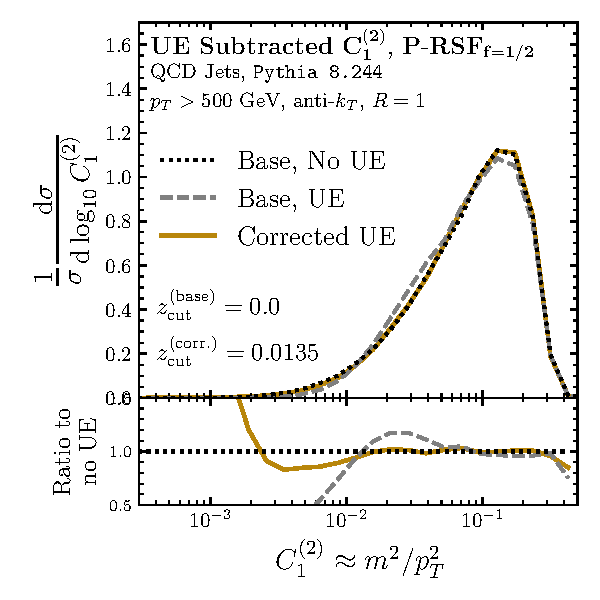
\includegraphics[width=.45\textwidth]{figures/piranha/responses/ue/c12_ratio_plots/rsf_half_zbase0.0_ratio_maintext}
        \label{fig:rss_ue_0}
    }
    \subfloat[][]{
        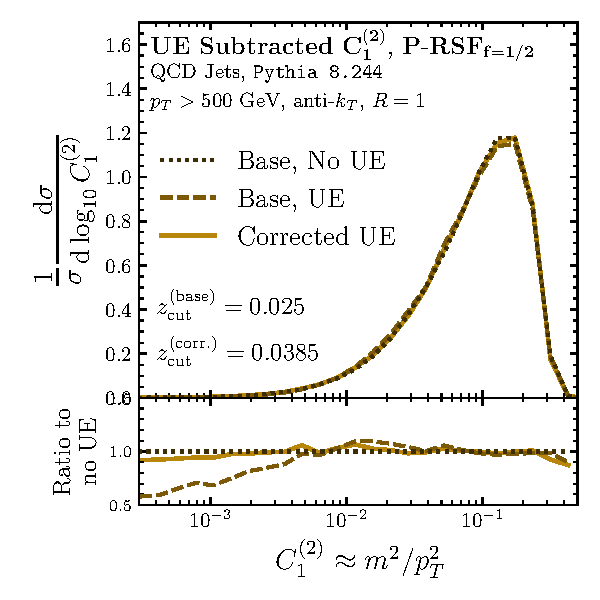
\includegraphics[width=.45\textwidth]{figures/piranha/responses/ue/c12_ratio_plots/rsf_half_zbase0.025_ratio_maintext}
        \label{fig:rss_ue_025}
    }
    \\
    \subfloat[][]{
        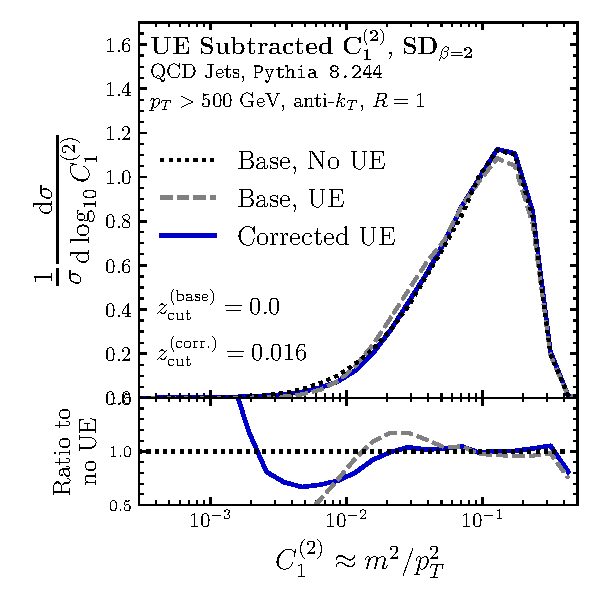
\includegraphics[width=.45\textwidth]{figures/piranha/responses/ue/c12_ratio_plots/sd2_zbase0.0_ratio_maintext}
        \label{fig:sd_ue_0}
    }
    \subfloat[][]{
        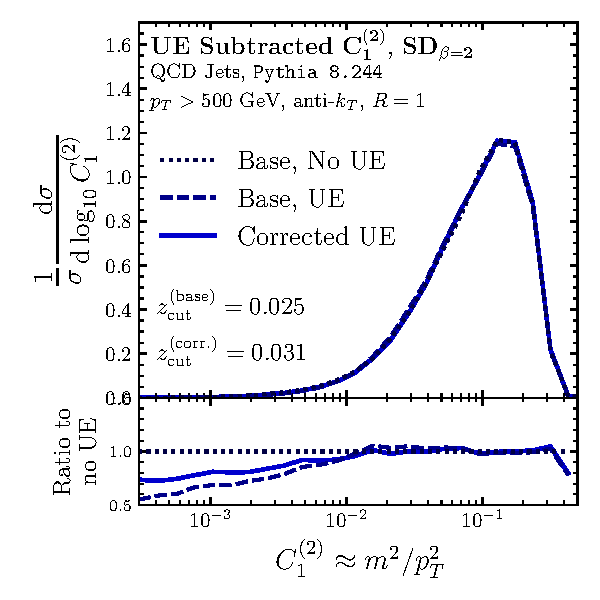
\includegraphics[width=.45\textwidth]{figures/piranha/responses/ue/c12_ratio_plots/sd2_zbase0.025_ratio_maintext}
        \label{fig:sd_ue_025}
    }
    \caption[The response of groomed substructure distributions of QCD jets to \glslink{ue}{the underlying event}, using \PRSF{1/2} and Soft Drop with \(\beta_{\rm SD} = 2\).]{
        The response of groomed substructure distributions of QCD jets to the underlying event (\gls{ue}), using \PRSF{1/2} (top row) and Soft Drop with \(\beta_{\rm SD} = 2\) (bottom row).
        %
        We examine the robustness of groomed substructure to the presence of \gls{ue} by comparing ``Base'' substructure distributions with and without \gls{ue} for fixed \(\zcut = z^{(\rm base)}_{\rm cut}\).
        %
        We also examine the possibility of adding \textit{additional} grooming to remove the effects of \gls{ue}, picking a \(z^{(\rm corr.)}_{\rm cut}\) that removes \gls{ue} to most accurately reproduce substructure distributions using \(\zcut = z^{(\rm base)}_{\rm cut}\) in the absence of \gls{ue}.
        %
        The left column shows the substructure distributions for \(z^{(\rm base)}_{\rm cut} = 0\), while the right column shows the substructure distributions for \(z^{(\rm base)}_{\rm cut} = 0.025\).
    }
    \label{fig:ue}
\end{figure}


\Fig{ue} compares base distributions to \gls{ue-corrected} for \PRSF{1/2} and Soft Drop.
%
\Figs{rss_ue_0}{sd_ue_0} examine the ability of the groomers to reproduce ungroomed base distributions, with \(\zcut^{(\rm base)} = 0\).
%
\Figs{rss_ue_025}{sd_ue_025} examine instead groomed base distributions with \(\zcut^{(\rm base)} = 0.025\).

\begin{figure}[]
    \subfloat[][]{
        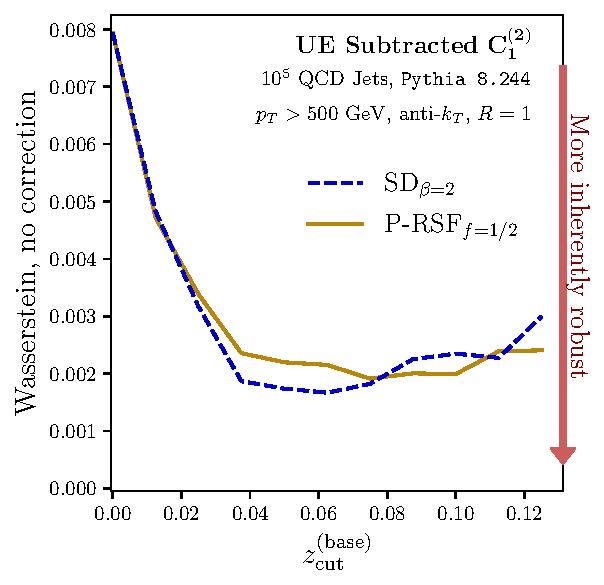
\includegraphics[width=.48\textwidth]{figures/piranha/responses/ue/wassersteins/wdists_maintype_correctedFalse}
        \label{fig:ue_wasser_nocorrection}
    }
    \subfloat[][]{
        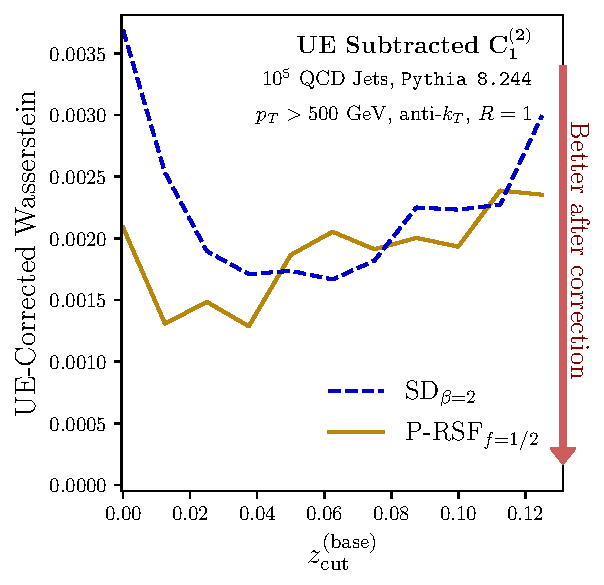
\includegraphics[width=.48\textwidth]{figures/piranha/responses/ue/wassersteins/wdists_maintype_correctedTrue}
        \label{fig:ue_wasser_uecorrection}
    }
    \caption[Behaviors of the Wasserstein distance, in arbitrary units, between the \(C_1^{(2)}\) distribution to \gls{ue} before and after \glslink{ue-corrected}{UE correction}, with \SD{2} and \PRSF{1/2}, as a function of the base amount of grooming \(\zcut^{(\rm base)}\).]{
        The behavior of the Wasserstein distance, in arbitrary units, between the \(C_1^{(2)}\) distribution: (a) before \glslink{ue-corrected}{UE correction}, and (b) after \glslink{ue-corrected}{UE correction}, for \SD{2} and \PRSF{1/2} as a function of the base amount of grooming \(\zcut^{(\rm base)}\).
        %
        In (b), a lower \glslink{ue-corrected}{UE-corrected} Wasserstein distance quantitatively indicates better correction against the effects of UE:
        %
        the substructure distribution of \glslink{ue-corrected}{UE-corrected} jets more closely resembles the substructure distribution of jets without \gls{ue}.
    }
    \label{fig:ue_2}
\end{figure}


\Figs{ue_wasser_nocorrection}{ue_wasser_uecorrection} quantify the effectiveness and robustness of \PRSF{1/2} and Soft Drop as a function of \(\zcut^{(\rm base)}\) by studying the un-corrected Wasserstein distance and the \glslink{ue-corrected}{UE-corrected} Wasserstein distance, respectively.
%
\Fig{ue_wasser_uecorrection} shows the \glslink{ue-corrected}{UE-corrected} Wasserstein distance as a function of \zcut, and suggests that \PRSF{1/2} is better at correcting for UE when \(\zcut^{(\rm base)} \lesssim .05\), and that \SD{0} and \PRSF{1/2} have similar \glslink{ue-corrected}{UE correction} ability for values of \(\zcut^{(\rm base)}\) between 0.05 and .1.

We note that we expect hard-cutoff groomers to be generically more \textit{robust} to the presence of \gls{ue} because even at fixed \zcut, they can remove an arbitrary amount of energy due to soft, wide-angle radiation in an event.
%
We correspondingly expect that hard-cutoff groomers require less additional grooming to remove the effects of \gls{ue}.
%
\PIRANHA{} groomers, on the other hand, cannot remove arbitrary amounts of energy from an event;
%
we expect that we must always slightly increase the strength of \PIRANHA{} grooming to soak up \gls{additive-contamination} from \gls{ue}.
%
We demonstrate that hard-cutoff groomers indeed require less additional \(\delta\zcut\) for optimal \glslink{ue-corrected}{UE correction} in \Fig{uefrenzy} of \App{uefrenzy}.

    We also point out that Recursive Subtraction techniques that are more geared towards the removal of the soft and wide-angle radiation which is characteristic of \gls{ue} may perform even better in \glslink{ue-corrected}{UE correction}.
    %
    In hard-cutoff grooming, for example, Soft Drop with \(\beta_{\rm SD} > 0\) preferentially grooms wide-angle radiation, Soft Drop with positive \(\beta_{\rm SD}\) is particularly well suited to remove \gls{ue} (see, for example, \Fig{uefrenzy} of \App{uefrenzy}).
   %
   Perhaps P-RS grooming procedures that upgrade the parameter \(f_{\rm soft}\) of P-RSF into a function of the soft energy fraction \(z\) and the splitting angle \(\theta\) of a branch  (such as Hard-Balanced P-RSF, as in \Sec{rsf_discont}) may be more suited to the removal of soft wide-angle radiation from \gls{ue}.

   We have argued that \PRSF{1/2} and \SD{2} are comparable tools for the subtraction of \gls{ue} effects in jet substructure, though \PRSF{1/2} requires more tuning to achieve the same level of \glslink{ue-corrected}{UE correction}.
   %
   We emphasize that further investigation of such P-RS algorithms might improve the ability of \PIRANHA{} in the tagging of boosted objects and beyond.


%=====================================
% Mass Resolution:
%=====================================
\subsection{Mass Extraction with Grooming: \texorpdfstring{\(W\)}{W} and Top Jets at the LHC}
\label{sec:pira-mass}
% TODO: add gls mass extraction to PIRANHA mass res section

    As a final case study, we explore the use of \PIRANHA{} grooming strategies in the tagging of boosted objects, another useful application of traditional grooming strategies such as Soft Drop.
   %
   We must once again overcome the subtlety that \PIRANHA{} grooming strategies remove energy proportional to the grooming parameter (such as \(\zcut\) in Recursive Safe Subtraction).
   %
   To successfully tag boosted objects decaying into jets, we must tune the grooming parameter for \PIRANHA{} strategies more than we would for Soft Drop.
   %
   Nonetheless, we examine the mass resolution of \PIRANHA{}-groomed jets from the decays of boosted \(W\) bosons and top quarks and discover that \PIRANHA{} may offer some advantages that are complementary to those of traditional grooming strategies.
   %
   The tagging procedure we implement in the following discussion is quite simple, however, and the applications of \PIRANHA{} in boosted object tagging should be subjected to a more complete analysis.

\begin{figure}[p]
    \subfloat[][]{
        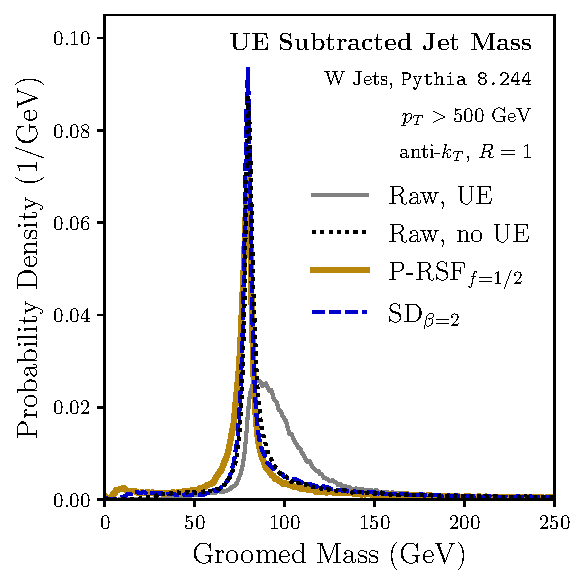
\includegraphics[width=.45\textwidth]{figures/piranha/responses/mass_resolution/w_mass_resolution}
        \label{fig:w_tagging_dist}
    }
    \subfloat[][]{
        \includegraphics[width=.45\textwidth]{figures/piranha/responses/mass_resolution/w_mass_roc}
        \label{fig:w_tagging_roc}
    }
    \\
    \subfloat[][]{
        \includegraphics[width=.45\textwidth]{figures/piranha/responses/mass_resolution/top_mass_resolution}
        \label{fig:top_tagging_dist}
    }
    \subfloat[][]{
        \includegraphics[width=.45\textwidth]{figures/piranha/responses/mass_resolution/top_mass_roc}
        \label{fig:top_tagging_roc}
    }
    \caption[A comparison of traditional and \PIRANHA{} grooming procedures in the tagging of boosted \(W\) bosons and top quarks.]
    {
         A comparison of traditional and \PIRANHA{} grooming procedures in the tagging of (top row) boosted \(W\) bosons and (bottom row) top quarks.
         %
          The data in the plots correspond to 100,000 jet events with \(p_T > 500\) GeV in \texttt{Pythia 8.244}.
          %
          The left column displays the mass distributions of \(W\) and top jets with and without \gls{ue}, and with \gls{ue} groomed away using either Soft Drop with \(\beta_{\rm SD} = 2\) or \PRSF{1/2} with additional post-processing discussed in the text.
          %
          The right column displays the relationship between background rejection and signal efficiency associated with \(W\) and top tagging, respectively, produced by considering symmetric windows around the mass of the relevant boosted object and comparing with a QCD background.
    }
    \label{fig:tagging}
\end{figure}

   In \Fig{tagging}, we assess the behavior of \PIRANHA{} in tagging boosted objects.
   %
   We focus on jets of \(p_T \geq 500\) GeV produced from the decays of \(W\) bosons and top quarks in \Figs{w_tagging_dist}{top_tagging_dist}, respectively.
   %
   We then plot the associated background rejection as a function of signal efficiency in \Figs{w_tagging_roc}{top_tagging_roc}.

To produce the groomed mass distributions of \Figs{w_tagging_dist}{top_tagging_dist}, we groom jets in the presence of \gls{ue}.
%
 Afterward, we rescale the mass of the jet to correct for the shift of the mass peak due to the removal of energy from the jet during grooming.
   %
   This rescaling procedure is necessary to reproduce the correct mass peak for \PRSF{1/2};
   %
   however, rescaling Soft Drop groomed mass distributions has a minimal effect since Soft Drop tends to remove wide-angle soft radiation without severely affecting radiation from the hard event.

   \Figs{w_tagging_dist}{top_tagging_dist} show rescaled mass distributions for each grooming algorithm for the value of \zcut{} that most precisely removes \gls{ue}, in the sense that it most closely reproduces the mass distribution of jets without \gls{ue}.
   %
   We find that the best performance is achieved by \(\zcut^{(\text{P-RSF}_{1/2})}=0.034\) and \(\zcut^{(\text{SD}_2)}=0.025\) when grooming W jets, and \(\zcut^{(\text{P-RSF}_{1/2})}=0.023\) and \(\zcut^{(\text{SD}_2)}=0.035\) when grooming top jets.
   %
   In each case, Soft Drop does not require any additional rescaling, while we find the best performance if we rescale the energy of \PRSF{1/2} groomed jet constituents by about \(+4\%\).

   In this simple context, \PRSF{1/2} offers slightly better background rejection for reasonable signal efficiencies.
   %
   We evince this in \Figs{w_tagging_roc}{top_tagging_roc}, where we show the signal efficiency versus background rejection curves associated with comparing signal W or top jets to QCD background, again with \(p_T \geq 500\) GeV.
   %
   Our tagging procedure is minimal:
   %
   we accept events within a symmetric window of width \(\delta m\) around the mass of the \(W\) boson or top quark, respectively, and \Figs{w_tagging_roc}{top_tagging_roc} are produced by varying the window size \(\delta m\).
   %
   For reasonable values of signal efficiency, between around 60\% and 90\%, the \PRSF{1/2} algorithm gives greater background rejection than Soft Drop.

   Again, the results in \Figs{w_tagging_dist}{top_tagging_dist} and \Figs{w_tagging_roc}{top_tagging_roc} suggest that \PRSF{1/2} and \SD{2} behave comparably as tools to remove the effects of \gls{ue} in jet mass distributions, and to tag underlying boosted object.
   %
   These results are preliminary, and to state these conclusions with more confidence will require more detailed tagging procedures than the simple algorithm described above.
   %
   We leave a more detailed study of the tagging potential of \PRSF{1/2} and \PIRANHA{} to future work.


%==============================================
\section{Connecting back out}
%==============================================
In this chapter, we explored jet grooming as a tool for illuminating the inner structure of jets in the presence of low-energy pollution.
%
We introduced traditional hard-cutoff jet grooming strategies and their analytic features, and proposed the paradigm of Pileup and Infra-red Radiation Annihilation (\PIRANHA{}) for continuous jet grooming.
%
Borrowing from the declustering properties of the popular \gls{soft-drop} algorithm for hard-cutoff jet grooming, we introduced Recursive Subtraction with a Fraction (P-RSF) as a family of new groomers motivated by the \PIRANHA{} paradigm.
%
Motivated by optimal transport theory and the \glslink{emd}{Energy Mover's Distance (EMD)} of \Reff{Komiske:2019fks}, we re-framed the \glslink{apollonius}{Apollonius Subtraction (P-AS)} and \glslink{ivs}{Iterated Voronoi Subtraction (P-IVS)} procedures of \Reff{Komiske:2020qhg} as implementations of the \PIRANHA{} paradigm.
%
We showed that a particular Recursive Subtractor, \PRSF{1/2}, overcomes the soft discontinuities of traditional hard-cutoff grooming procedures, and that general P-RSF algorithms only have soft discontinuities in suppressed regions of phase space.
%
We highlighted the unprecedented robustness of \PRSF{1/2} to \gls{hadronization}, \gls{deteffects}, and \glslink{pileup}{pileup}.
%
We showed also that \PRSF{1/2} may be able to correct for the presence of \glslink{ue}{the underlying event}.
%
Though hard-cutoff groomers may be more robust against effects from \gls{ue} without additional tuning, \PIRANHA{} groomers can be tuned to remove \gls{additive-contamination} from \glslink{ue}{the underlying event}.
%
We used the example of \gls{additive-contamination} from \gls{ue} to argue that \PIRANHA{} may also have applications in the tagging of boosted objects.

There are several immediately evident avenues for future phenomenological and theoretical exploration.
%
While we argued that P-RSF had more robust responses to \glspl{soft-distortion}, it will be interesting to quantify this including theoretical, model-dependent uncertainties.
%
For example, it will be interesting to study the robustness of \PRSF{1/2} to \gls{hadronization} when using different models of color recombination, with different \texttt{Pythia} tunes, and from the perspective of effective field theory as in \Reff{Hoang:2019ceu}.
%
Similarly, the effects of experimental detectors on \PRSF{1/2} groomed quantities must be explored with more realistic models of detector responses and compared in more detail with traditional grooming techniques.
%
More detailed studies of these model-dependent uncertainties may facilitate a more precise, and even process-dependent method to tune the parameters of \PIRANHA{} groomers such as P-RSF to the removal of \gls{pileup} and \gls{ue} in more realistic scenarios.

Designing and studying variants of P-RSF in which the amount of grooming for a particular emission depends on the angle of the emission, as in Soft Drop with \(\beta_{\rm SD} \neq 0\), and even the energy fraction, may be another easy way to improve the robustness and precision of P-RS algorithms in removing specific models of soft contamination.
%
Indeed, any method that varies \(f_{\rm soft}\), \(\zcut\), \(\rho\), or other parameters of the jet grooming procedure in a way that depends on more detailed information within the jet could be useful in more precise removal of contaminating radiation, such as the removal of \gls{pileup}, \gls{ue}, or the thermal noise that contaminates jets originating in heavy ion collisions.

   A first-principles calculation of Recursive Subtraction groomed jet observables will rely on analytic exploration of the elaborately correlated emissions of P-RS groomed jets, as well as contributions from non-global configurations.
%
We begin this journey in \App{calc}, but further exploration may depend on a more precise application of existing tools for jet substructure or even on newer tools in \gls{pqcd}, such as the techniques of \Reff{Larkoski:2015zka}.

The study of EMD-mode \PIRANHA{} grooming, introduced in \App{grooming_in_emd_mode}, is another interesting avenue for the development of continuous grooming techniques.
%
Unlike the \PIRANHA{} groomers explored in the main text, EMD-mode \PIRANHA{} groomers have the potential to remove an arbitrary amount of \(p_T\) from an event.
%
We look forward to future studies of EMD-mode grooming for its potential to address stochastic fluctuations in the levels of jet contamination.

Finally, the use of alternative methods for optimal transport, such as the EMD without the restriction of \(\beta = 1\) that we chose in this thesis, or the flexible and computationally efficient formalism of linearized optimal transport \cite{Cai:2020vzx,Cai:2021hnn,cai2022linearized,sarrazin2023linearized}, may offer new tools and additional insights into continuous grooming.

The \PIRANHA{} grooming strategy has intricate geometric origins, but its goal is simple: the optimal and continuous removal of contaminating low-energy radiation.
%
We hope that the simple strategies and examples of continuous grooming discussed in this thesis may provide and inspire new tools for clear communication between experimental results and theoretical predictions regarding our microscopic universe.


Our appetite has now been whet for continuous probes of jet substructure.
%
In the next chapter, we pursue a complementary approach to designing continuous collider observables that are insensitive to the presence of low-energy pollution.
%
Rather than directly removing soft radiation, we will \textit{ignore} it by designing energy-weighted correlators which directly probe the correlations of high-energy structures within jets.


% TODO: where do I put SECTION ACKNOWLEDGMENTS?
%\acknowledgments

%The authors would like to express their gratitude to Matthew LeBlanc, Jennifer Roloff, and the ATLAS Jet Definitions subgroup for valuable discussions, and to Nima Zardoshti for raising insightful questions during LHCP 2022.
%%
%We would also like to thank Pier Monni for helpful discussions regarding resummation, and Sean Benevedes and Rikab Gambhir for engaging conversations and careful readings of the manuscript.
%%
%Finally, we extend our appreciation to an anonymous referee whose thoughtful comments and feedback contributed to improving the quality and clarity of this thesis and especially of \Sec{discontinuity}.
%%
%This work was supported by the Office of Nuclear Physics of the U.S. Department of Energy (DOE) under grant DE-SC-0011090, by the DOE Office of High Energy Physics under grants DE-SC0012567 and DE-SC0019128, and by the National Science Foundation under Cooperative Agreement PHY-2019786 (The NSF AI Institute for Artificial Intelligence and Fundamental Interactions, \url{http://iaifi.org}).



% %%%%%%%%%%%%%%%%%%%%%%%%%%%%%%%%%%%%
% Appendices
% %%%%%%%%%%%%%%%%%%%%%%%%%%%%%%%%%%%%
\begin{subappendices}

%==============================================
\section{Samples}
%==============================================
In the studies of this section, we use \texttt{Pythia 8.244} \cite{Sjostrand:2014zea} with the default 4C tune \cite{Corke:2010yf}, and work with samples of QCD quark and gluon jets without multiple parton interactions.
%
We consider jets with transverse momentum \(p_T > 500\) GeV, maximum pseudorapidity \(|\eta| < 4\), and clustered with the anti-\(k_T\) algorithm \cite{Cacciari:2008gp} with \(R = 1\);
%
we then re-cluster using the Cambridge-Aachen algorithm \cite{Dokshitzer:1997in,Wobisch:1998wt}.
%
Our analyses focus on Soft Drop with \(\beta_{\rm SD} = 2\) as a representative for traditional grooming procedures and on Balanced Recursive Subtraction (\PRSF{1/2}) as a representative for \PIRANHA{} grooming;
%
the Balanced Recursive Subtraction algorithm is available on GitHub \cite{piranhagithub}.

We study the responses of groomed jets to \glspl{soft-distortion} through three qualitatively different lenses:
\begin{itemize}
    \item \textbf{Energy Flow: EMD}
    \\
    %
    To understand the overall response of groomed jet energy flow to soft radiation, we use the EMD of \Sec{emd}.
    %
    The EMD between two jets bounds the difference of a large class of IRC-safe observables between the jets and provides an observable-independent tool to study the robustness of different grooming procedures to the presence of soft contamination.\footnote{
    In particular, the EMD of \Sec{emd} tends to reflect the response of extensive properties of jets, as we see concretely in our examples;
    %
    a less concrete way to see this is by directly looking at \Eq{EMD_def_1}, and noticing that the EMD has units of energy.
    }

    \item \textbf{Extensive Properties: \(p_T\)}
    \\
    To understand how the extensive properties of groomed jets are modified by soft contamination, we examine the responses of the transverse momentum of groomed jets.
    %
    We are concerned in particular with the amount by which transverse momentum in the presence of contamination, \(\widetilde{p_T}\), is shifted relative to the associated un-contaminated value, \(p_T\):
    \begin{align}
        \Delta p_T = \widetilde{p_T}- p_T
        %\frac{\Delta p_T}{p_T} = \frac{\widetilde{p_T}- p_T}{p_T}
        .
        \label{eq:pt_response}
    \end{align}
   \(p_T\) indicates transverse momentum in the absence of distortion or contamination and \(\widetilde{p_T}\) captures the response of transverse momentum to different sources of low-energy physics.
   %
   This is specified more precisely in each of the subsequent sections.

    \item \textbf{Substructure: \(C_1^{(\varsigma)}\)}
    \\
    We use jet substructure to capture the response of the intensive properties of jets to contaminating radiation.
    %
    In particular, we study the response of the two-prong energy correlation functions (ECFs) of \Reff{Larkoski:2013eya}:
    %
    \begin{equation}
        C_1^{(\varsigma)}
        =
        \frac{1}{2}\frac{\sum_{i=1}^M\sum_{j=1}^M p_{T,\,i}\ p_{T,\,j}\ \left(R_{ij}/R_0\right)^\varsigma}{p_{T,\,{\rm tot.}}^2}
        \label{eq:ECFdefn_pheno}
        .
    \end{equation}
    %
    \(p_{T,\,i}\) represents the fraction of the jet transverse momentum carried by particle \(i\), \(R_{ij}\) indicates the rapidity-azimuth distance between particles \(i\) and \(j\), and the sum is over all particles in the jet.
    %
    In the limit of jets that are central (\(y = 0\)) and narrow (have jet radius \(R_0 \ll 1\)), we can write the ECFs in the approximate form of \Eq{GECFdefn_lo}.
    %
    As a concrete example of the response of substructure to soft radiation, we focus on \(\Delta C_1^{(2)} = \widetilde{C_1^{(2)}} - C_1^{(2)} \approx \Delta\left(m^2 / p_T^2\right)\), where a tilde again indicates the associated observable in the presence of a particular source of low-energy physics, while the absence of a tilde indicates the absence of low-energy effects.
\end{itemize}

We emphasize that in all of our phenomenological studies (except our studies of \glslink{ue}{the underlying event} in \Secs{ue}{pira-mass}), we examine how each source of contamination leads to changes on a ``per-jet'' level, rather than at the level of distributions of observables.
%
In particular, we examine the EMD between each jet before and after contamination, and the changes in \(p_T\) and \(C_1^{(2)}\) induced by contamination for individual jets.
%
To the best of our knowledge, the effects of \gls{hadronization} on a per-jet basis have not been studied in this way before, as the sensitivity of groomed jets to \gls{hadronization} is often studied instead at a statistical level by studying the distributions of groomed jet observables.
%
Therefore, the results we present offer a more detailed examination of the effects of the \gls{hadronization} model of \texttt{Pythia 8.244};
%
however, these results may not be precisely reflected solely by the statistical changes in distributions of groomed jet observables that are induced by \gls{hadronization}.



%==============================================
\section{Grooming in EMD Mode}
%==============================================
\label{app:grooming_in_emd_mode}
In this appendix, we describe another route for developing \PIRANHA{} groomers:
%
\textit{EMD mode}.
%
EMD-mode grooming produces a groomed event with a fixed EMD relative to its ungroomed counterpart, and furnishes a complementary approach to ``\(p_T\)-mode'' groomers.
%
We provide a conceptual introduction to EMD-mode grooming below, leaving an exploration of the phenomenological implications of EMD mode to future work.


The \PIRANHA{} groomers described above all subtract a fixed amount of transverse momentum from the energy flow of an event.
%
Let us call them \textit{\(p_T\)-mode groomers}.
%
\(p_T\)-mode grooming gives us a great deal of control over the amount of energy we remove from an event.
%
When using \PIRANHA{} groomers in \(p_T\) mode to remove \gls{additive-contamination}, however, this precise control over \(\Delta p_T\) leads to additional complications;
%
since \gls{additive-contamination} may add arbitrary amounts of contaminating soft radiation to an event, removing a fixed amount of \(p_T\) from the contaminated event may not be the best strategy for reproducing the un-contaminated event.
%
These complications lead to important considerations when using \PIRANHA{} for \gls{pu-mitigation}, as in \Sec{pira-pu} and \App{pufrenzy}, and they are especially disadvantageous when using \PIRANHA{} to correct for the presence of \glslink{ue}{the underlying event}, as in \Sec{pira-ue} and \App{uefrenzy}.

Grooming in EMD mode is a complementary approach that allows \PIRANHA{} groomers to remove arbitrary amounts of soft radiation from an event.
%
\PIRANHA{} in EMD mode therefore furnishes a conceptually interesting alternative for continuous grooming.

First, let us briefly review how the \(p_T\)-mode algorithms we have presented for \gls{apollonius}, \gls{ivs}, and P-RS all subtract a fixed amount of transverse momentum, \(\Delta p_T = \rho A_{\rm tot}\), or \(\Delta p_T = \zcut p_T\), from the event under consideration.
%
\begin{itemize}
\item
\gls{apollonius} subtracts the pre-specified \(p_T\) all at once by finding the Apollonius regions associated with the event, as in \Sec{as}.
%
\item
\gls{ivs} subtracts the pre-specified \(p_T\) by subtracting \(p_T\) from each particle in the event until it removes a particle, and then continues recursively until the specified \(p_T\) has been removed, as in \Sec{ivs}.
%
\item
P-RS subtracts the pre-specified \(p_T\) by recursively assigning fractions of the total \(p_T\) to be removed to each branch of the jet tree until it reaches the final-state particles of the jet, as in \Sec{recursive-subtraction}.
\end{itemize}


The approach for EMD-mode grooming is quite similar.
%
In EMD mode, however, each algorithm continues until a specific amount of EMD has been subtracted from the event, often in an iterative procedure.
%
As a concrete example, let us construct the algorithm for \gls{ivs} in EMD mode, or \gls{ivs}\(^{(\rm EMD)}\):
%
\begin{enumerate}
    \item
    \gls{ivs}\(^{(\rm EMD)}\) finds the Voronoi diagram for the event, as discussed in \Sec{ivs}, and indexes the steps of the algorithm by \(n\), starting at \(n=1\).
    %
    We define the energy flow of the algorithm after step \(n\) is completed by \(\mathcal{E}_n\), where \(\mathcal{E}_0\) is the energy flow of the original event.
    %
    We also define the EMD between \(\mathcal{E}_{n-1}\) and \(\mathcal{E}_n\) as \({\rm EMD}_n\).

    \item
    \gls{ivs}\(^{(\rm EMD)}\) attempts to modify the \(p_T\) of every particle in the event in the same way as \gls{ivs} in \(p_T\)-mode:
    \begin{align}
	p_{T\,i}^{(n)} = p_{T\,i}^{(n-1)} - \rho^{(n)} A^{(n-1)}_i,
	\label{eq:ivs_emd}
    \end{align}
    where the \(p_{T\,i}^{(n-1)}\) and \(A^{(n-1)}\) are the transverse momenta/Voronoi areas after step \(n-1\), and
    \begin{align}
        \rho^{(n)}
        =
        \min_i p^{(n)}_{T\,i}/A^{(n)}_i
        ,
    \end{align}
    in analogy with \Eq{ivs2}.
    %
    As in \Sec{ivs}, \(\rho^{(n)}\) describes the maximum \(p_T\) that may be subtracted from an event before one of the particles in the event is groomed away entirely.

    \item
    \gls{ivs}\(^{(\rm EMD)}\) next calculates \({\rm EMD}_n\) for this proposed groomed event, and asks whether it has subtracted a total EMD of \( {\rm EMD}_{\rm cut}\) from the event.
    %
    If \(\sum_{k = 1}^n {\rm EMD}_n < {\rm EMD}_{\rm cut}\), \gls{ivs}\(^{(\rm EMD)}\) has not yet subtracted the full \({\rm EMD}_{\rm cut}\) from the event.
    %
    In this case, we have more grooming to do:
    %
    \gls{ivs}\(^{(\rm EMD)}\) continues recursively, going back to the first step of the algorithm.

    \item
    If \(\sum_{k = 1}^n {\rm EMD}_k > {\rm EMD}_{\rm cut}\), \gls{ivs}\(^{(\rm EMD)}\) has subtracted too much EMD from the event.
    %
    In this case, \gls{ivs}\(^{(\rm EMD)}\) revises its proposed groomed event at this step in the algorithm by evaluating the value of \(\rho^{(n)}\) that would give \(\sum_{k = 1}^n {\rm EMD}_k > {\rm EMD}_{\rm cut}\), and finding the associated groomed event by using \Eq{ivs_emd}.
    %
    It returns the resulting event as the final groomed event.
\end{enumerate}
As in \gls{ivs}, \gls{ivs}\(^{(\rm EMD)}\) does not need to re-compute the Voronoi diagram from scratch at each step of the algorithm.
%
Similarly, our procedure for finding the value of \(\rho^{(n)}\) that subtracts the correct amount of total EMD in the final step of the algorithm is computationally efficient, and does not rely on a complete re-evaluation of the EMD at each step of the algorithm.


At present, we do not have an implementation of P-RS in EMD mode.
%
That said, we expect that the generalization of EMD-mode grooming to P-RS and P-RSF will be similar:
%
at step \(n\) of the EMD mode algorithm, we perform grooming with the maximum value of \(z_{\rm cut}\) until a particle would be removed, and define EMD\(_n\) as the EMD between the energy flows at steps \(n-1\) and \(n\) of the grooming.
%
If the sum of the subtracted EMDs is greater than EMD\(_{\rm cut}\), \(\sum_{k = 1}^n {\rm EMD}_k > {\rm EMD}_{\rm cut}\),
%
we must compute the value of \(z_{\rm cut}\) that fixes \({\rm EMD}_n > {\rm EMD}_{\rm cut} - \sum_{k = 1}^{n-1} {\rm EMD}_k \), groom with this value of \(z_{\rm cut}\), and return the resulting groomed event.
%
Otherwise, if \(\sum_{k = 1}^n {\rm EMD}_k < {\rm EMD}_{\rm cut}\), we would continue grooming recursively.

We hope that future exploration of EMD-mode grooming may offer additional utility in the use of continuous grooming in the subtraction of \gls{additive-contamination}, and in the mitigation of obfuscating radiation in general.

%==============================================
\section[Feeding Frenzy: Plethora of \textsc{Piranha}]{Feeding Frenzy: Plethora of PIRANHA}
%==============================================
\label{app:feedingfrenzy}
In this appendix, we present a brief collection of additional results regarding the responses of \PIRANHA{} and Soft Drop groomers to \glspl{soft-distortion} and \gls{additive-contamination}.
%
We extend the results in the main text by comparing \PRSF{1/2}, the focus of our phenomenological studies in the main text, to three groups of grooming algorithms:
%
\begin{itemize}
    \item
    \textbf{Hard-Cutoff Groomers:}
    \SD{0}, \SD{1}, and \SD{2};

    \item
    \textbf{Fully Continuous Groomers:}
    \gls{apollonius} and \gls{ivs};

    \item
    \textbf{Recursive Subtractors:}
    \PRSF{0}, \PRSF{1/2}, \PRSF{3/4}, and \PRSF{1}.
\end{itemize}
In our \glslink{pileup}{pileup} studies, we also count Constituent Subtraction (CS) \cite{Berta:2014eza} among the continuous groomers due to its continuity properties in the continuum limit.
%
The comparisons of this appendix demonstrate that the conclusions we drew in the main text by comparing \PRSF{1/2} to \SD{2} seem to hold in greater generality:
%
\PIRANHA{} groomers tend to have more robust responses to \glspl{soft-distortion} and \gls{additive-contamination} than traditional grooming methods.
%
Furthermore, the responses of \PRSF{1/2} are similar to the responses of the fully continuous groomers \gls{apollonius} and \gls{ivs} (and CS, in the case of \gls{pu-mitigation});
%
each of the \PIRANHA{} algorithms we explore in this appendix are available on GitHub \cite{piranhagithub}.

As in the main text, we first extend our results involving \gls{hadronization} corrections (\Sec{pira-hadronization}) and all-charged corrections (\Sec{pira-neutral}) to explore how several choices of grooming and grooming parameters may respond to \glspl{soft-distortion}.
%
We then begin our discussion of \gls{additive-contamination} by providing more detail regarding our \glslink{pileup}{pileup} studies:
%
we explain in greater detail our procedure for \gls{pu-mitigation} used in \Sec{pira-pu} and extend our results to several groomers and values of \(\langle n_{\rm PU}\rangle\).
%
Finally, we similarly explore how different groomers respond to \glslink{ue}{the underlying event}, extending the results of \Sec{pira-ue}.


\begin{figure}[p]
    \centering
    \subfloat[]{
        \includegraphics[width=.32\textwidth]{figures/piranha/feeding_frenzy/pvh/sigmaemdsdtype-ph}
    }
    \subfloat[]{
        \includegraphics[width=.32\textwidth]{figures/piranha/feeding_frenzy/pvh/sigmaemdpiratype-ph}
    }
    \subfloat[]{
        \includegraphics[width=.32\textwidth]{figures/piranha/feeding_frenzy/pvh/sigmaemdrsftype-ph}
    }
    \\
    \subfloat[]{
        \includegraphics[width=.32\textwidth]{figures/piranha/feeding_frenzy/pvh/sigmaptsdtype-ph}
    }
    \subfloat[]{
        \includegraphics[width=.32\textwidth]{figures/piranha/feeding_frenzy/pvh/sigmaptpiratype-ph}
    }
    \subfloat[]{
        \includegraphics[width=.32\textwidth]{figures/piranha/feeding_frenzy/pvh/sigmaptrsftype-ph}
    }
    \\
    \subfloat[]{
        \includegraphics[width=.32\textwidth]{figures/piranha/feeding_frenzy/pvh/sigmac12sdtype-ph}
    }
    \subfloat[]{
        \includegraphics[width=.32\textwidth]{figures/piranha/feeding_frenzy/pvh/sigmac12piratype-ph}
    }
    \subfloat[]{
        \includegraphics[width=.32\textwidth]{figures/piranha/feeding_frenzy/pvh/sigmac12rsftype-ph}
    }
    \caption[Per-jet \gls{hadronization} responses of the EMD, \(\Delta p_T\), and \(\Delta C_1^{(2)}\) using a plethora of fully continuous, hard-cutoff, and recusive subtraction grooming strategies.]{
    Per-jet \gls{hadronization} responses of \PIRANHA{} and traditional groomers for (top row) EMD, (middle row) \(\Delta p_T\), and (bottom row) \(C_1^{(2)}\);
    %
    we compare \PRSF{1/2} to (left column) hard-cutoff groomers, (middle column) fully continuous groomers, and (right column) recursive subtractors.
    %
    For brevity in this appendix, we focus on the variance of the shifts in each observable due to \gls{hadronization} in groomed jets.
    %
    The red arrows indicate the direction corresponding to better performance.
}
\label{fig:pvhfrenzy}
\end{figure}



\begin{figure}[p]
    \subfloat[]{
        \includegraphics[width=.32\textwidth]{figures/piranha/feeding_frenzy/avc/sigmaemdsdtype-avc}
    }
    \subfloat[]{
        \includegraphics[width=.32\textwidth]{figures/piranha/feeding_frenzy/avc/sigmaemdpiratype-avc}
    }
    \subfloat[]{
        \includegraphics[width=.32\textwidth]{figures/piranha/feeding_frenzy/avc/sigmaemdrsftype-avc}
    }
    \\
    \subfloat[]{
        \includegraphics[width=.32\textwidth]{figures/piranha/feeding_frenzy/avc/sigmaptsdtype-avc}
    }
    \subfloat[]{
        \includegraphics[width=.32\textwidth]{figures/piranha/feeding_frenzy/avc/sigmaptpiratype-avc}
    }
    \subfloat[]{
        \includegraphics[width=.32\textwidth]{figures/piranha/feeding_frenzy/avc/sigmaptrsftype-avc}
    }
    \\
    \subfloat[]{
        \includegraphics[width=.32\textwidth]{figures/piranha/feeding_frenzy/avc/sigmac12sdtype-avc}
    }
    \subfloat[]{
        \includegraphics[width=.32\textwidth]{figures/piranha/feeding_frenzy/avc/sigmac12piratype-avc}
    }
    \subfloat[]{
        \includegraphics[width=.32\textwidth]{figures/piranha/feeding_frenzy/avc/sigmac12rsftype-avc}
    }
\caption[Responses to the exclusion of neutral particles of the EMD, \(\Delta p_T\), and \(\Delta C_1^{(2)}\) using a plethora of fully continuous, hard-cutoff, and recusive subtraction grooming strategies.]{
    Same as \Fig{pvhfrenzy}, but for jet responses to the exclusion of neutral particles.
}
\label{fig:avcfrenzy}
\end{figure}

\subsection{Response to Soft Distortions}
In the main text, we made the argument that continuity provides more predictable responses to \glspl{soft-distortion};
%
we therefore focus on the fluctuations induced by \glspl{soft-distortion} by studying the standard deviations of the groomed EMD and \(C_1^{(2)}\) as a function of \zcut.

\Fig{pvhfrenzy} shows the fluctuations in the parton-hadron groomed EMD and the parton-hadron \(\Delta C_1^{(2)}\), as discussed in \Sec{pira-hadronization}, for a variety of grooming options.
%
The first column of \Fig{pvhfrenzy} demonstrates that \PRSF{1/2} groomed jets tend to have significantly smaller fluctuations due to \gls{hadronization}, echoing the conclusions of \Sec{pira-hadronization}.
%
We note that \SD{2} is significantly more robust to \gls{hadronization} than \SD{0} when considering extensive observables (EMD and \(p_T\)).
%
The second two columns of \Fig{pvhfrenzy} show that the \PIRANHA{} groomers we consider all have similar \gls{hadronization} responses in the considered range of \zcut.

\Fig{avcfrenzy} presents the all-charged groomed EMD and \(\Delta C_1^{(2)}\) as discussed in \Sec{pira-neutral}.
%
The first column again shows that \PRSF{1/2} experiences significantly smaller fluctuations due to the exclusion of neutral particles than Soft Drop, and the second two columns show similar responses for all \PIRANHA{} groomers.


\subsection{Pileup Response}
\label{app:pufrenzy}

We now provide more detail regarding our \gls{pileup} mitigation procedure.
%
As discussed in \Sec{pira-pu}, we use the dijet and minimum bias events of \Reff{Soyez:2018opl} to study the effects of \gls{pileup}.
%
We use the \texttt{GridMedianBackgroundEstimator} (GMBE) method of \texttt{FastJet} \cite{Cacciari:2011ma} to provide a rough estimate, \(\rho_{\rm GMBE}\), of the energy density of \gls{additive-contamination} due to \glslink{pileup}{pileup} in each jet we would like to groom.
%
However, since GMBE is designed to provide an estimate of the contaminating energy in an entire event,\footnote{
Note that \texttt{FastJet} also supports \textit{Jet} Median Background Estimation (JMBE), which is more suited to the task of estimating the contaminating energy density in each jet.
%
We were unable to find \texttt{Python} support for JMBE and used the method detailed here as a replacement.
} we improve upon the GMBE procedure by optimizing a correction factor that scales the GMBE estimate for each groomer.
%
We optimize the correction factor for each groomer by considering its action on 100,000 events, throwing away events where the presence of \gls{pileup} changes which jet within the dijet has more energy, and implementing the following procedure:

\begin{enumerate}
    \item
    For each epoch \(i\) during our optimization, estimate the contaminating energy density due to \gls{pileup} within a jet,
    \begin{align}
        \rho_{\rm PU}[\mathcal E] = \frac{p_T^{\rm (PU~in~jet)}}{A_{\rm jet}}
        ,
    \end{align}
    that needs to be applied by a groomer \(g\) to accurately remove \gls{pileup} contamination as
    \begin{align}
        \rho^{{\rm(epoch}\,i)}_{\rm est.}[\mathcal E ; g)
        =
        \rho_{\rm GMBE}\,[\mathcal E] f_i(g)
        ,
    \end{align}
    where we use parentheses to indicate that \(\rho_{\rm est.}\) and \(f\) are functions of the groomer \(g\), and square brackets to indicate that the energy densities \(\rho\) are functionals of the energy flow \(\mathcal E\).
    %
    Since we are using jets clustered using the anti-\(k_t\) algorithm, we may take the jet area to be \(\pi R_{\rm jet}^2\) \cite{Cacciari:2008gp}.

    \item
    Introduce a new epoch every 1,000 events we consider, by adjusting our proposed correction factor \(f_i\) to
    \begin{align}
        f_{i + 1}
        =
        f_i + r_{\rm learn}
        \left\langle \frac{\Delta \rho}{\rho} \right\rangle_i
        \label{eq:epochcorrectionfactor}
        ,
    \end{align}
    where the angular brackets indicate an average over the jets considered during epoch \(i\), \(\Delta \rho\) indicates the difference in \(p_T\) density in a \glslink{pileup}{pileup} subtracted event and a hard event,
    \begin{align}
        \Delta \rho
        =
        \frac{\Delta p_T}{A_{\rm jet}}
        =
        \frac{p_T^{\rm(groomed~PU)} - p_T^{\rm(hard)}}{A_{\rm jet}}
        ,
    \end{align}
    and \(r_{\rm learn}\) is a learning rate which we set to 1/3.


    \item
    At the end of the final epoch, save the final correction factor \(f_{\rm learned}(g)\) for each groomer.

    \item
    Perform a new analysis of the ability of each groomer to remove \gls{pileup} by estimating the optimal \(\rho\) required for PU-subtraction as
    \begin{align}
        \rho_{\rm est.}[\mathcal E ; g)
        =
        \rho_{\rm GMBE}\,[\mathcal E] f_{\rm learned}(g)
        .
    \end{align}
    We recall for completeness that \(
    	z_{\rm cut}
	=
	\rho_{\rm est.} A_{\rm jet}/p_T^{(\rm jet)}
    \).

\end{enumerate}



\begin{figure}[p]
\centering
    \subfloat[]{
        \includegraphics[width=.32\textwidth]
        {figures/piranha/feeding_frenzy/pu/sdtype_emd_npu_shifts}
    }
    \subfloat[]{
        \includegraphics[width=.32\textwidth]
        {figures/piranha/feeding_frenzy/pu/piratype_emd_npu_shifts}
    }
    \subfloat[]{
        \includegraphics[width=.32\textwidth]
        {figures/piranha/feeding_frenzy/pu/rsftype_emd_npu_shifts}
    }
    \\
    \subfloat[]{
        \includegraphics[width=.32\textwidth]
        {figures/piranha/feeding_frenzy/pu/sdtype_dpt_npu_shifts}
    }
    \subfloat[]{
        \includegraphics[width=.32\textwidth]
        {figures/piranha/feeding_frenzy/pu/piratype_dpt_npu_shifts}
    }
    \subfloat[]{
        \includegraphics[width=.32\textwidth]
        {figures/piranha/feeding_frenzy/pu/rsftype_dpt_npu_shifts}
    }
    \\
    \subfloat[]{
        \includegraphics[width=.32\textwidth]
        {figures/piranha/feeding_frenzy/pu/sdtype_dc1_npu_shifts}
    }
    \subfloat[]{
        \includegraphics[width=.32\textwidth]
        {figures/piranha/feeding_frenzy/pu/piratype_dc1_npu_shifts}
    }
    \subfloat[]{
        \includegraphics[width=.32\textwidth]
        {figures/piranha/feeding_frenzy/pu/rsftype_dc1_npu_shifts}
    }
    \caption[Average per-jet \glslink{pileup}{pileup}-induced shifts in the EMD, \(\Delta p_T\), and \(C_1^{(2)}\).]{
    Average per-jet \glslink{pileup}{pileup}-induced shifts in (top row) EMD, (middle row) \(\Delta p_T\), and (bottom row) \(C_1^{(2)}\);
    %
    we compare \PRSF{1/2} to (left column) hard-cutoff groomers, (middle column) fully continuous groomers, and (right column) recursive subtractors, as discussed in \Sec{pira-pu} and \App{feedingfrenzy}.
    %
    The red arrows indicate the direction corresponding to better performance.
}
\label{fig:pufrenzy_ave}
\end{figure}


\begin{figure}[p]
\centering
    \subfloat[]{
        \includegraphics[width=.32\textwidth]
        {figures/piranha/feeding_frenzy/pu/sdtype_emd_npu_stds}
    }
    \subfloat[]{
        \includegraphics[width=.32\textwidth]
        {figures/piranha/feeding_frenzy/pu/piratype_emd_npu_stds}
    }
    \subfloat[]{
        \includegraphics[width=.32\textwidth]
        {figures/piranha/feeding_frenzy/pu/rsftype_emd_npu_stds}
    }
    \\
    \subfloat[]{
        \includegraphics[width=.32\textwidth]
        {figures/piranha/feeding_frenzy/pu/sdtype_dpt_npu_stds}
    }
    \subfloat[]{
        \includegraphics[width=.32\textwidth]
        {figures/piranha/feeding_frenzy/pu/piratype_dpt_npu_stds}
    }
    \subfloat[]{
        \includegraphics[width=.32\textwidth]
        {figures/piranha/feeding_frenzy/pu/rsftype_dpt_npu_stds}
    }
    \\
    \subfloat[]{
        \includegraphics[width=.32\textwidth]
        {figures/piranha/feeding_frenzy/pu/sdtype_dc1_npu_stds}
    }
    \subfloat[]{
        \includegraphics[width=.32\textwidth]
        {figures/piranha/feeding_frenzy/pu/piratype_dc1_npu_stds}
    }
    \subfloat[]{
        \includegraphics[width=.32\textwidth]
        {figures/piranha/feeding_frenzy/pu/rsftype_dc1_npu_stds}
    }
\caption[Standard deviations of per-jet \glslink{pileup}{pileup}-induced shifts in the EMD, \(\Delta p_T\), and \(C_1^{(2)}\).]{
    Same as \Fig{pufrenzy_ave}, but for the standard deviation of the \glslink{pileup}{pileup}-induced shifts.
}
\label{fig:pufrenzy_stddev}
\end{figure}


In \Figs{pufrenzy_ave}{pufrenzy_stddev}, we present results on \gls{pileup} mitigation using the optimization procedure described above for a variety of groomers, as an extension of the discussion in \Sec{pira-pu}.
%
We focus on the \glslink{pusubevent}{PU-subtracted} EMD, the \glslink{pusubevent}{PU-subtracted} \(\Delta p_T\), and the \glslink{pusubevent}{PU-subtracted} \(\Delta C_1^{(2)}\) as a function of the average number of \gls{pileup} events \(\langle n_{\rm PU} \rangle\).

The \PIRANHA{} groomers displayed in \Fig{pufrenzy_ave}, together with CS, tend to perform only slightly better than the traditional groomers, on average, in removing \glslink{pileup}{pileup};
%
both \PIRANHA{} and traditional groomers have been tuned so that \(\langle \Delta p_T\rangle=0\), and this tuning is reflected by the relatively small changes to the extensive properties and even the substructure of the \glslink{pusubevent}{PU-subtracted} jets.
%
The notable exception is \PRSF{0}.
%
Since \PRSF{0} preferentially grooms away hard radiation, it is poorly suited to grooming away the low-energy \gls{additive-contamination} that is contributed by \glslink{pileup}{pileup}, and it performs more poorly than other \PIRANHA{} groomers in reproducing both extensive and substructure properties of \glslink{pusubevent}{PU-subtracted} jets.

However, \Fig{pufrenzy_stddev} shows that \PIRANHA{} groomers and CS are more \textit{reliable} PU mitigators than traditional groomers:
%
the standard deviations in the shifts of \glslink{pusubevent}{PU-subtracted} extensive and substructure properties tend to be significantly smaller for \PIRANHA{} groomers than for traditional groomers.
%
Again, \PRSF{0} is a noticeable exception and is less reliable as a PU mitigator than either \PIRANHA{} or traditional grooming methods.


\begin{figure}[t!]
    \subfloat[]{
        \includegraphics[width=.5\textwidth]{figures/piranha/feeding_frenzy/runtime/runtimes_npu50}
    }
    \subfloat[]{
        \includegraphics[width=.5\textwidth]{figures/piranha/feeding_frenzy/runtime/average_runtimes}
    }
    \caption[
    Runtimes for \PIRANHA{} algorithms, and comparison to some traditional grooming and \gls{pu-mitigation} algorithms.]{
    Runtimes for \PIRANHA{} algorithms, and comparison to some traditional grooming and \gls{pu-mitigation} algorithms.
    %
    (a) shows the probability density for the logarithm of the runtime for each algorithm when \(\langle n_{\rm PU} = 50\rangle\), where \(n_{\rm PU}\) is the average number of \glslink{pileup}{pileup} events.
    %
    (b) shows the average runtime for each algorithm as a function of \(\langle n_{\rm PU} \rangle\).
    %
    Runtimes are shown for the \texttt{Pythia 8.185} datasets of \Reff{Soyez:2018opl}, and we simulate \glslink{pileup}{pileup} by layering a Poisson-distributed number of minimum-bias events over a hard dijet event.
    }
    \label{fig:runtimes}
\end{figure}


We also briefly present results for the runtimes of the grooming algorithms discussed in this paper, including the Constituent Subtraction (CS) \gls{pu-mitigation} algorithm, as a function of the amount of \gls{additive-contamination} in events with \gls{pileup}.
%
In particular, \Fig{runtimes} displays the properties of runtimes for grooming algorithms functioning as \glslink{pileup}{pileup} mitigators as we vary the average number of layered minimum bias events, \(\langle n_{\rm PU} \rangle\).
%
The tree-based grooming strategies, such as Soft Drop and P-RS, are the fastest.
%
\gls{ivs} is an order of magnitude slower.
%
Finally, \gls{apollonius} and CS are the slowest, with runtimes of \(\mathcal O({\rm 1s})\) even for a reasonable number of \glslink{pileup}{pileup} events.
%
The combination of high speed and high performance of balanced P-RS provides simple preliminary evidence for their utility in the removal of \glslink{pileup}{pileup}.
\\~\\

\begin{figure}[p]
    \centering
    \subfloat[]{
        \includegraphics[width=.32\textwidth]{figures/piranha/responses/ue/wassersteins/wdists_sdtype_correctedFalse}
        \label{fig:uefrenzy_wasserstein_sd}
    }
    \subfloat[]{
        \includegraphics[width=.32\textwidth]{figures/piranha/responses/ue/wassersteins/wdists_piratype_correctedFalse}
        \label{fig:uefrenzy_wasserstein_pira}
    }
    \subfloat[]{
        \includegraphics[width=.32\textwidth]{figures/piranha/responses/ue/wassersteins/wdists_rsftype_correctedFalse}
    }
    \\
    \subfloat[]{
        \includegraphics[width=.32\textwidth]{figures/piranha/responses/ue/wassersteins/wdists_sdtype_correctedTrue}
        \label{fig:uefrenzy_correctedwasserstein_sd}
    }
    \subfloat[]{
        \includegraphics[width=.32\textwidth]{figures/piranha/responses/ue/wassersteins/wdists_piratype_correctedTrue}
        \label{fig:uefrenzy_correctedwasserstein_pira}
    }
    \subfloat[]{
        \includegraphics[width=.32\textwidth]{figures/piranha/responses/ue/wassersteins/wdists_rsftype_correctedTrue}
    }
    \\
    \subfloat[]{
        \includegraphics[width=.32\textwidth]{figures/piranha/responses/ue/delta_zcuts/zcuts_sdtype}
    \label{fig:uefrenzy_deltazcut_sd}
    }
    \subfloat[]{
        \includegraphics[width=.32\textwidth]{figures/piranha/responses/ue/delta_zcuts/zcuts_piratype}
    \label{fig:uefrenzy_deltazcut_pira}
    }
    \subfloat[]{
        \includegraphics[width=.32\textwidth]{figures/piranha/responses/ue/delta_zcuts/zcuts_rsftype}
    }
    \caption[Wasserstein distance between jet \(C_1^{(2)}\) distributions in the presence of \gls{ue} with and without \glslink{ue-corrected}{UE correction}.]{
    Wasserstein distance between jet \(C_1^{(2)}\) distributions (top row) without \glslink{ue-corrected}{UE correction} and (middle row) with \glslink{ue-corrected}{UE correction}, and (bottom row) the optimal value of \(\delta \zcut\) for \glslink{ue-corrected}{UE correction}.
    %
}
\label{fig:uefrenzy}
\end{figure}


\subsection{Underlying Event Response}
\label{app:uefrenzy}

For \glslink{ue}{the underlying event}, we present results for the Wasserstein distances between substructure distributions with and without \gls{ue}, discussed in \Sec{pira-ue}, as well as the additional grooming \(\delta\zcut\) required for optimal \glslink{ue-corrected}{UE correction}.
%
We collect these results in \Fig{uefrenzy}.

In each of the plots, a lower value along the $y$-axis -- of either the Wasserstein distance or the optimal additional \(\delta\zcut\) -- indicates a desirable property for \glslink{ue-corrected}{UE correction}.
%
A lower Wasserstein distance without \glslink{ue-corrected}{UE correction} indicates inherent robustness of the groomer to the presence of \gls{ue}.
%
A lower \glslink{ue-corrected}{UE-corrected} Wasserstein distance indicates that the groomer is able to better correct for the presence of \gls{ue}.
%
Finally, a lower \(\delta\zcut\) indicates greater robustness against \gls{ue}:
%
less additional grooming must be applied for \glslink{ue-corrected}{UE correction}.

Notably, \Fig{uefrenzy_correctedwasserstein_sd} shows that the \glslink{ue-corrected}{UE-corrected} Wasserstein distance of \PRSF{1} is smaller than that of Soft Drop for several values of \(\beta_{\rm SD}\) and a range of \(z_{\rm cut}^{\rm (base)}\), indicating that \PRSF{1} is a more delicate tool for the removal of \gls{additive-contamination} due to \gls{ue}.
%
However, \gls{ivs} and \gls{apollonius} perform even better at \gls{ue} removal, as shown in \Fig{uefrenzy_correctedwasserstein_pira}.
%
It may be that simple improvements to P-RS that emulate the features of \gls{ivs} and \gls{apollonius}, such as the ``Hard-Balanced Recursive Subtractors'' mentioned briefly in \Sec{rsf_discont}, may lead to even better performance in \gls{ue} removal.
%
Finally, while the P-RSF groomers generally exhibit similar performance in \glslink{ue-corrected}{UE correction}, \PRSF{0} performs poorly at \glslink{ue-corrected}{UE correction} and is extremely sensitive to the effects of \gls{ue};
%
this is unsurprising, as \PRSF{0} deliberately grooms away hard radiation and leaves in soft radiation, such as the radiation contributed by \gls{ue}.

Since the procedure we use to study the ability of each groomer to remove \gls{ue} is based on a computationally expensive optimization of \(\delta\zcut\), the plots we show in \Fig{uefrenzy_deltazcut_sd} have some unphysical, jagged behavior, especially in the second two rows.
%
We expect that with a dedicated study with better statistics that the jagged behavior of these plots will be smoothed, but that the qualitative nature of our conclusions will remain unchanged.


\end{subappendices}


% %%%%%%%%%%%%%%%%%%%%%%%%%%%%%%%%%%%%
% Problems
% %%%%%%%%%%%%%%%%%%%%%%%%%%%%%%%%%%%%
\begin{problems}

\makeprob{Constant-Cutoff Substructure at MLL}{constant-cutoff-mll}{
    Find the radiator for \glslink{constant-cutoff}{constant-cutoff-groomed} angularities at MLL.
    %
    Include running coupling effects and freeze the coupling at a non-perturbative scale \(\mu_\text{NP}\).
    %
    Write the associated MLL cumulative distribution and probability distribution in closed form.
}


\makeprob{Constant-Subtraction Substructure at MLL}{constant-subtraction-mll}{
    Find the radiator for \glslink{constant-subtraction}{constant-subtraction-groomed} angularities at MLL.
    %
    Include running coupling effects and freeze the coupling at a non-perturbative scale \(\mu_\text{NP}\).
    %
    Write the associated MLL cumulative distribution and probability distribution in closed form.
}



\makeprob{\(\star\) Multiplicity of Simple Groomed Jets \(\star\)}{simple-groomed-multiplicity}{
    Find the multiplicity distribution for constant-cutoff-groomed jets using the principles of the partonic cascade.
    %
    You may wish to refer to the solution of \Prob{subjet-multiplicity}.
}



\makeprob{\(\star\star\star\) Resummed Recursive Subtraction \(\star\star\star\)}{resummed-rs}{
    Derive resummed analytic expressions, potentially in terms of a radiator or other integrals to be evaluated numerically, for \gls{gecf} distributions of \gls{rsf}-groomed jets which include the effects of multiple emissions.
}


\end{problems}
